\documentclass[a4paper,12pt]{report}

\usepackage{fontspec}
\usepackage{setspace}
\usepackage{polyglossia}
\setmainlanguage{hungarian}
\usepackage[a4paper,top=2cm,left=3cm,bottom=2cm,right=2cm]{geometry}
\usepackage{graphicx}
\usepackage{float}
\usepackage{hyperref}
\usepackage{amsmath}
\usepackage{amssymb}
\usepackage{booktabs}
\usepackage{array}
\usepackage{tabularx}
\usepackage{longtable}
\usepackage{caption}
\usepackage{enumitem}
\usepackage{listings}
\usepackage{xcolor}
\usepackage{titlesec}
\usepackage{url}
\usepackage{rotating}

\titleformat{\chapter}[hang]{\normalfont\bfseries\LARGE}{\thechapter.}{1em}{}
\setcounter{tocdepth}{2}
\setlist[itemize]{noitemsep, topsep=4pt}
\setlength{\parskip}{6pt}
\setlength{\parindent}{0pt}
\graphicspath{{assets/demo_shots/}{assets/diagrams/}}
\setmainfont{Calibri}
\setsansfont{Calibri}
\setmonofont{Consolas}
\setstretch{1.15}

\lstset{
  basicstyle=\ttfamily\small,
  breaklines=true,
  frame=single,
  columns=fullflexible,
  keepspaces=true
}

\newcommand{\diagramfigure}[2]{
\begin{figure}[H]
\centering
\includegraphics[width=0.92\textwidth]{#2}
\caption{#1}
\end{figure}
}

\newcommand{\placeholder}[2]{%
\begin{figure}[H]
\centering
\fbox{\parbox{0.85\textwidth}{\centering\vspace{2.2cm}%
\textbf{[PLACEHOLDER]}\par\vspace{0.4em}{\small #1}\vspace{2.2cm}}}%
\caption{#2}
\end{figure}%
}


\begin{document}

\begin{titlepage}
    \centering
    {\LARGE UMFST \par}
    \vspace{1.2cm}
    {\Large Informatikai Kar \par}
    \vspace{3.3cm}
    {\huge\bfseries Premade Graph Explorer\par}
    \vspace{0.5cm}
    {\Large League of Legends játékoskapcsolatok, teljesítménymutatók és gráfanalitikai kiterjesztések\par}
    \vfill
    {\Large Készítette: Tamási Krisztián-Erik\par}
    \vspace{2.3cm}
    {\large Marosvásárhely, 2026\par}
\end{titlepage}

\tableofcontents
\clearpage


\chapter{Bevezetés}

\section{Problémafelvetés}

A kompetitív online játékok egyik visszatérő problémája, hogy a résztvevők nagyon erős véleményeket fogalmaznak meg egymás teljesítményéről, miközben ehhez rendszerint csak részleges, szubjektív és rövid távú benyomások állnak rendelkezésre. Egy elveszített mérkőzés után gyorsan megjelenik a bűnbakkeresés, de sokkal ritkábban történik meg az, hogy a játékosok valóban adatalapon próbálják megérteni, mi történt a meccsben, hogyan teljesítettek ők maguk, és hogyan helyezhető el ez a teljesítmény egy tágabb közösségi hálózatban.

A \emph{League of Legends} különösen érdekes terep ehhez, mert egyszerre tartalmaz rendkívül gazdag mérkőzésadatokat, ismétlődő csapattársi és ellenfél-kapcsolatokat, valamint olyan társas mintázatokat, amelyek gráfként ábrázolhatók és elemezhetők. Ha egy játékos hosszabb időn keresztül ugyanazokkal az emberekkel kerül egy meccsbe (akár szövetségesként, akár ellenfélként), akkor ebből egy olyan kapcsolati háló építhető fel, amely túlmutat az egyetlen mérkőzés pillanatnyi statisztikáin.

Ebből a felismerésből indult a dolgozat: a cél nem egyszerűen egy újabb meccsnéző vagy statisztikai felület volt, hanem egy olyan rendszer, amely a valós mérkőzéstörténetből játékoshálót épít, ezt a hálót gráfelméleti és rendszerszintű szemlélettel elemzi, majd az eredményeket egy vizuálisan erős, ugyanakkor védhető frontend felületen mutatja meg.

\section{Motiváció}

A projekt mögött részben személyes indíttatás húzódik. Rangsorolt meccsek után visszatérő kérdés volt, hogy a sorozatos negatív találkozások véletlen-e, vagy van mögöttük valami szerkezet -- esetleg ugyanazok az emberek kerülnek újra és újra egymás mellé, csak ezt a matchmaking felülete nem mutatja meg. Ez önmagában persze nem tudományos kérdés, de kiindulópontként elég volt. Ha a Riot API részletes meccsadatokat ad, és ezek ismétlődő játékoskapcsolatokat tartalmaznak, akkor ezekből elvileg gráf építhető -- és ha gráf van, akkor már van mit elemezni.

A rendszer végül jóval nagyobbra nőtt, mint amire számítottam. Ami kezdetben gyors adatvizualizációnak indult, az fokozatosan külön adatgyűjtő réteggé, normalizált pontszámítási pipeline-ná, SQLite-alapú perzisztenciává, Rust futtatókörnyezetté és többoldalas React frontenddé alakult. A Python réteg adatgyűjtési és legacy-kompatibilitási szerepben maradt meg -- ez nem tervezett döntés volt, hanem a fejlesztés természetes következménye.

\section{A dolgozat célja}

A dolgozat célja egy olyan, valós mérkőzésadatokra épülő, többkomponensű rendszer bemutatása, amely:

\begin{itemize}
    \item League of Legends meccsekből játékosok közötti kapcsolatokat gyűjt és tisztít,
    \item a játékosokhoz szerepkör-érzékeny teljesítménymutatókat rendel,
    \item az ismétlődő együtt- és egymás ellen játszásból gráfot épít,
    \item a gráfot klaszterekre, útvonalakra, core-periphery mintázatokra és kutatási célú metrikus kapcsolatokra bontja,
    \item a számításigényes részeket determinisztikus, exportálható és újrafuttatható módon kezeli,
    \item az eredményeket interaktív, de nem UI-első szemlélettel mutatja meg.
\end{itemize}

Fontos szempont volt végig, hogy a rendszer ne csak vizuálisan legyen érdekes, hanem a mögötte lévő döntések is megindokolhatók legyenek: honnan jönnek az adatok, hogyan számolódnak a pontszámok, mit jelent pontosan egy él a gráfban, és mit nem.

\section{Kutatási kérdések}

A jelen dolgozat a következő kutatási kérdésekre keres választ:

\begin{itemize}
    \item Hogyan építhető fel valós League of Legends mérkőzéstörténetből egy olyan játékosháló, amely nem pusztán az együtt játszást, hanem az ellenfél-kapcsolatokat is megőrzi?
    \item Milyen módon lehet a játékosok teljesítményét úgy pontozni, hogy az figyelembe vegye a tényleges szerepkört, de közben megmaradjon értelmezhetőnek?
    \item Mennyiben indokolt a rendszer különböző rétegeit Python, SQLite, Node.js, Rust és React komponensekre bontani?
    \item Mutat-e a jelenlegi gráf pozitív asszortativitást a \texttt{opscore} és \texttt{feedscore} tekintetében?
    \item Miben különbözik a \texttt{flexset} és a \texttt{soloq} kapcsolati szerkezete, és mennyiben írható le a \texttt{flexset} asszociatív core-periphery játékosgráfként?
\end{itemize}

\section{A dolgozat hozzájárulása}

A dolgozat gyakorlati és szakmai hozzájárulásai a jelenlegi implementáció alapján a következők:

\begin{itemize}
    \item több-adatkészletes, regiszter-alapú mérkőzésgyűjtési és feldolgozási architektúra;
    \item szerepkörérzékeny, adatbázis-alapú \texttt{opscore}/\texttt{feedscore} normalizáció;
    \item Rust-központú Graph V2 gráfépítés, klaszterezés és artifact-export SQLite perzisztenciával;
    \item Rust oldali útvonalkeresés BFS, Dijkstra, kétirányú keresés, egzakt A*, asszortativitás és Brandes-központisági támogatással;
    \item \texttt{flexset} és \texttt{soloq} dataset-összehasonlítás asszociatív gráfértelmezéssel;
    \item játékosteljesítményre számolt asszortativitási elemzés több gráfmódban;
    \item előre kiszámított 3D globális gráfnézet és többoldalas, kutatásbarát frontend.
\end{itemize}

\begin{figure}[H]
    \centering
    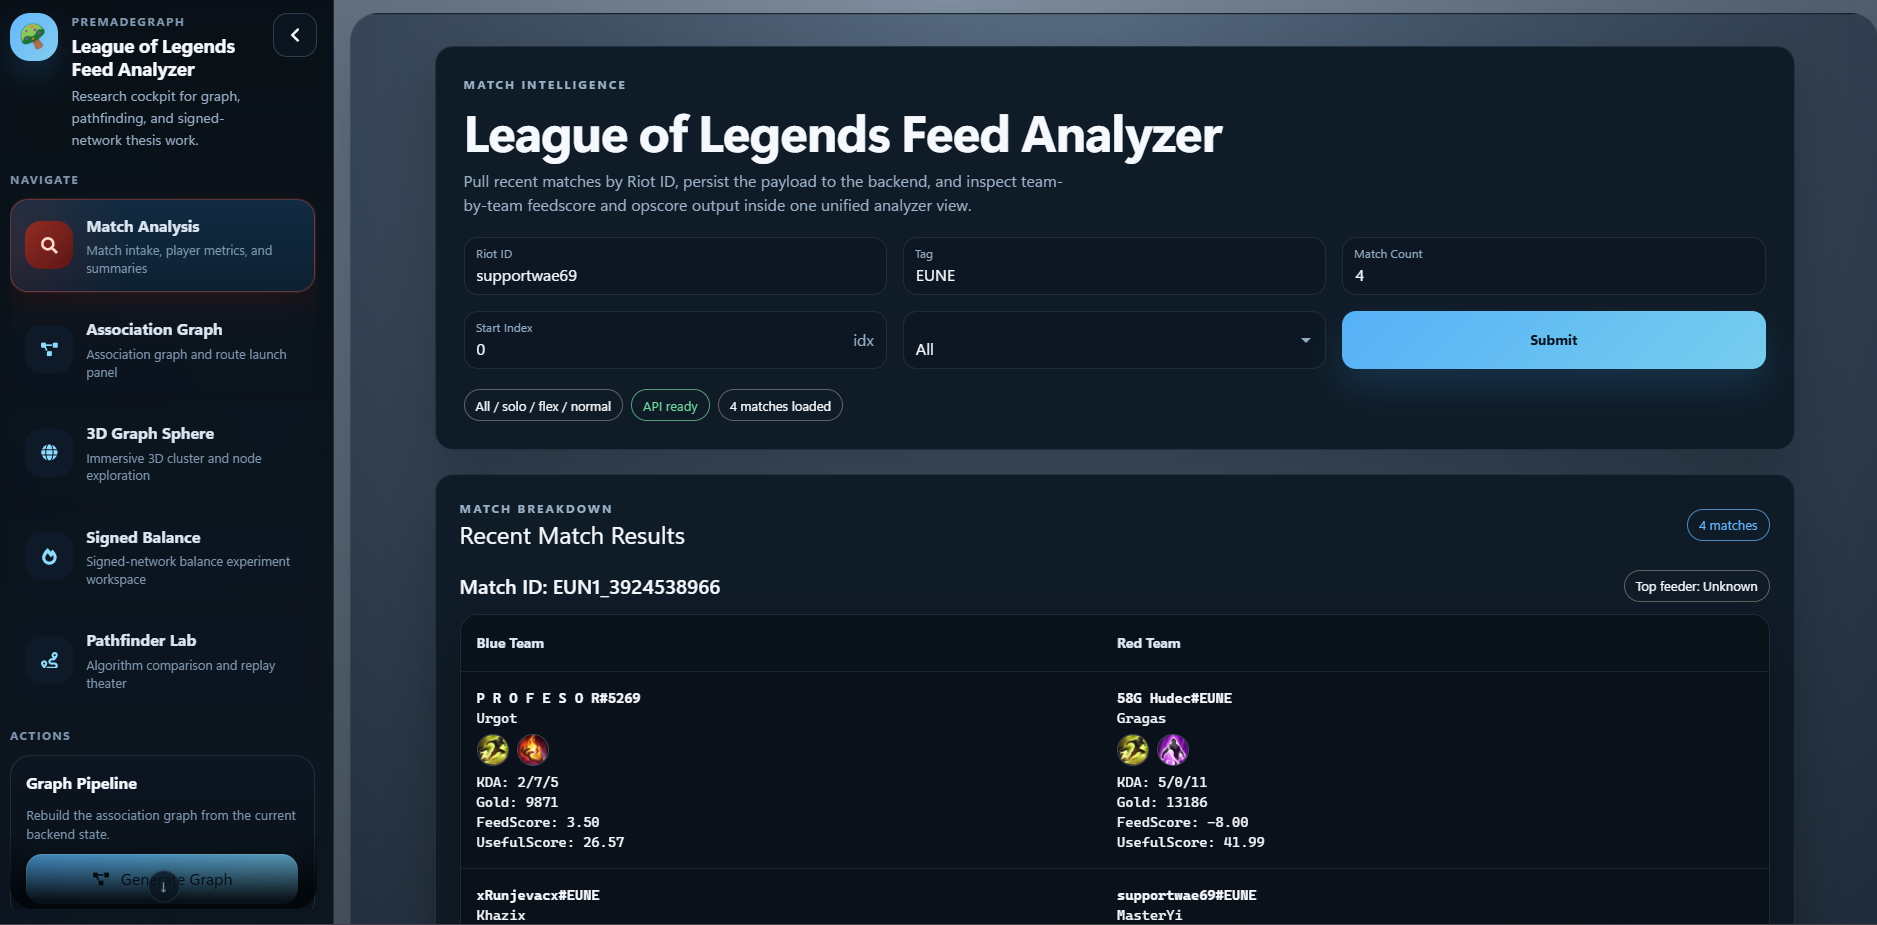
\includegraphics[width=0.92\textwidth]{match-analysis-page.png}
    \caption{A jelenlegi frontend egyik belépési pontja: meccselemzési és adatgyűjtési felület}
\end{figure}

\chapter{Problémafelvetés és motiváció}

\section{Miért nem elég egy hagyományos statisztikai oldal?}

A legtöbb, játékosoknak szánt statisztikai felület egyetlen mérkőzésre, egyetlen rangsorra vagy néhány alapmutatóra szűkíti le az értelmezést. Ez önmagában hasznos lehet, de nem válaszolja meg azt a kérdést, amely a projekt egészét végigkísérte: vajon a mérkőzések mögött kirajzolódik-e egy tartós társas szerkezet, és ha igen, ez a szerkezet hogyan kapcsolódik a teljesítményhez?

A \emph{Premade Graph} két egymástól nem független problémával szembesül. Az egyik adatmérnöki jellegű: a nyers Riot API válaszokból valahogy olyan adatkorpuszt kell felépíteni, ahol a játékosok azonosítása, a meccsek tárolása és a gráfprojekció újrafuttatható módon működik -- nem csak egyszer, hanem bővíthető és ellenőrizhető formában. A másik inkább kutatási: mit lehet egyáltalán állítani ezekből az adatokból, ami nem egyszerűen látványos, hanem valóban alátámasztható is.

Ez az oka annak, hogy a dolgozat fókusza tudatosan nem egyetlen UI-oldal vagy egyetlen algoritmus. A projekt értéke éppen abban áll, hogy az adatgyűjtés, a tisztítás, a pontszámítás, a gráfépítés, a klaszterezés, a futásidejű analitika és a vizualizáció ugyanannak a rendszernek az egymásra épülő rétegei.

\section{A projekt szokatlan és érdekes volta}

A szakdolgozat témája azért különösen érdekes, mert a kiinduló adathalmaz nem egyszerű játékoslista, hanem ismétlődő interakciós háló. A rendszer ugyanazt a két játékost nemcsak egyszeri ellenfelekként látja, hanem potenciális visszatérő szövetségesként, visszatérő ellenfélként, klasztertagként, hídcsúcsként vagy egy nagyobb globális hálózat részeként is.

Ez több okból ad erős szakdolgozati alapot:

\begin{itemize}
    \item a League of Legends mérkőzésadatai elég gazdagok ahhoz, hogy valódi teljesítményprofilok legyenek számíthatók;
    \item a visszatérő együttjátszás és egymás elleni előfordulás gráfelméleti szempontból értelmezhető kapcsolatokat hoz létre;
    \item a szövetségesi és ellenfél-jelleg együttese miatt a projekt nem csak súlyozott, hanem többféle kapcsolatprojekcióként is vizsgálható;
    \item a rendszer implementációs oldalon is érdekes, mert több nyelv és futtatókörnyezet közötti felelősségmegosztást kell megindokolni.
\end{itemize}

Ez a kombináció ritkább, mint elsőre látszik. Sok játékelemző projekt vagy a vizuális oldalnál áll meg, vagy csak egy-egy táblázatos mutatóig jut el. Itt viszont ugyanannak a rendszernek része a nyers adatgyűjtés, a szerepkörérzékeny score-réteg, a klaszterezés, az útvonalkeresés, az asszortativitási analitika, a Brandes-központiság és a 3D globális megjelenítés.

\section{A központi szakdolgozati állítás}

A dolgozat fő tézise az, hogy \emph{a valós mérkőzéstörténetből felépített League of Legends játékosháló egyszerre kezelhető mint asszociatív játékosgráf, mint teljesítményprofilokkal dúsított adatstruktúra, és mint rendszertechnikai szempontból komoly, többnyelvű analitikai platform}.

Ez három irányban bontható ki. A hálózati irány azt vizsgálja, hogy az ismétlődő együttjátszás és egymás elleni előfordulás mérhető szerkezeti mintázatot alkot-e -- a \texttt{flexset} adatkészleten ez leginkább asszociatív core-periphery szerkezetként mutatkozik meg, ahol a központban hídgazdag, visszatérő ally-csoportok sűrűsödnek. A metrikai irány a \texttt{feedscore} és \texttt{opscore} pontszámokra épül: ezek nem tökéletes teljesítménymutatók, de elég konzisztensek ahhoz, hogy gráfanalitikai bemenetként használhatók legyenek. A rendszertechnikai irány pedig azt indokolja, miért szükséges Python, SQLite, Node/Express, Rust és React együttese -- nem eszközpreferencia miatt, hanem mert a különböző részfeladatok eltérő természete ezt kívánja meg.

\section{Hatókör és korlátok}

A projekt viszonylag nagy rendszer, és könnyen csúszhat abba a hibába, hogy minden meglévő ötlet kész eredményként szerepeljen. A dolgozat igyekszik ezt elkerülni. Ami ténylegesen fut és ellenőrizhető, az kész állapotként szerepel. Ami megvan a repositoryban, de a jelenlegi adatpillanatképben nincs érdemi kimenete, az korábbi vagy kiegészítő modulként jelenik meg. Amit a fejlesztési tervek jövőbeli célként fogalmaznak meg, az nem szerepel kész feature-ként.

Konkrét példa: a klaszterekhez kötött ország- és régióelemzés kódja megvan, de az ellenőrzött adatbázisban a \texttt{country} mező nem tartalmazott értékelhető adatot, ezért ez a vonal kísérleti modulként van jelölve.

\section{A dolgozat szerkezete}

A dolgozat logikája a projekt fejlődését követi. Először a problémafelvetés és a szakirodalmi háttér kerül bemutatásra, majd a Riot API-ra épülő adatforrások és a korai pipeline. Ezt követően a pontozási rendszer, a gráfépítés és a régi ország-alapú elemzési ág tárgyalása következik. A középső fejezetek az architektúra evolúcióját, a több-adatkészletes modellt, az SQLite perzisztenciát és a Rust futtatókörnyezetet tárgyalják. Végül külön fejezetek mutatják be a Pathfinder Labot, a 3D bird's-eye sphere nézetet, az asszortativitási és központisági elemzéseket, valamint a strukturális egyensúly módszertani visszaminősítését, majd a validációt, a rendszerszintű értékelést és a jövőbeli fejlesztéseket.

\chapter{Szakirodalmi háttér}

\section{Hálózatkutatás és közösségszerkezet}

A gráfok társas kapcsolatok modellezésében régóta központi szerepet játszanak. A videojátékos közösségek esetében különösen izgalmas kérdés, hogy a játékosok közötti ismétlődő interakciók mennyiben alkotnak felismerhető struktúrákat, szubközösségeket, hidakat és lokális mintázatokat. Girvan és Newman klasszikus munkája rámutatott arra, hogy a hálózat élei nem pusztán kapcsolódási elemek, hanem közösségszerkezetet leíró, eltérő fontosságú viszonyok is lehetnek \cite{girvannewman}. Fortunato átfogó áttekintése pedig jól összefoglalja, miért központi probléma a közösségdetektálás a modern hálózatelemzésben \cite{fortunato2010}.

A jelen projektben a közösségfogalom nem öncélú. Azért fontos, mert a többször ismétlődő kapcsolatokra épülő játékoscsoportok értelmezhetőbbé teszik a nagyméretű hálózatot, segítenek elkülöníteni a valós kapcsolati magokat a zajtól, és támaszt nyújtanak a later\-i útvonal- és analitikai számításoknak.

\section{Közösségdetektálás és modularitás}

A korai Python oldali populációs klaszterezés a NetworkX \textit{greedy\_modularity\_communities} eljárását használta, amely a Clauset--Newman--Moore-féle mohó modularitásmaximalizálási megközelítésre épül \cite{clauset2004,networkx_greedy}. Ez tudatos kompromisszum volt: nem a leglátványosabb, hanem gyorsan magyarázható és reprodukálható megoldás. A jelenlegi futásidejű gráfállapotot a Rust motor önállóan, a meccs-JSON fájlokból és az SQLite-adatbázisból építi fel; Python ebben a szerepben lassú és nehezen skálázható lett volna. A Python pipeline szerepe ezért legacy/populációs közösségek és kompatibilitási exportok előállítása.

A modularitás-optimalizáció ismert korlátait sem hagyhatók figyelmen kívül: Fortunato és Barthelemy eredménye szerint a felbontási korlát miatt kisebb, de valós szerkezetek a globális optimum érdekében összeolvadhatnak \cite{fortunato_barthelemy2007}. A \textit{python\_population} klasztereket ezért nem szabad ontológiai "igazi közösségként" kezelni, inkább a választott gráf, súlymodell és heurisztika melletti legjobb, reprodukálható populációs partícióként.

\section{Asszortativitás}

Newman munkája az asszortatív keveredést olyan hálózati jelenségként írja le, amikor a kapcsolódó csomópontok hasonló vagy éppen eltérő tulajdonságúak \cite{newman2003}. A jelen projekt ezt a játékosok teljesítménymutatóira alkalmazza: nem az a kérdés, hogy a magas fokszámú csúcsok kapcsolódnak-e egymáshoz, hanem az, hogy a gráfban összekapcsolt játékosok hasonló \textit{opscore} vagy \textit{feedscore} értékeket hordoznak-e.

A dolgozat két gráfmódot különböztet meg: a \textit{social-path} csak a pozitív, szövetségesi támaszú kapcsolatokra épít, a \textit{battle-path} az összes ismétlődő együtt- vagy egymás ellen játszást figyelembe veszi. Az asszortativitás mértéke e két módban eltérhet, ami önmagában is informatív.

\section{Esport-analitika és játékos-teljesítménymérés}

A League of Legends és az általánosabb MOBA-játékok esport-analitikája önálló kutatási területté vált. Mora-Cantallops és Sicilia átfogó irodalmi áttekintése megmutatja, hogy a MOBA-játékok egyedi kombinációt kínálnak verseny, együttműködés, játékosélmény és társas interakció között, és ez a kombináció különlegesen gazdag adatforrást teremt empirikus vizsgálatokhoz \cite{moracantallops2019}.

A játékos-teljesítmény modellezése Novak és munkatársai munkájában is megjelenik: profi League of Legends meccsekre kidolgozott teljesítménymodellek rámutatnak, hogy a domainspecifikus változók és a strukturált adatfeldolgozás fontosabb, mint az általános statisztikai modellek \cite{novak2022}. Ez erősíti a jelen projekt szerepkörérzékeny pontozási megközelítésének indokoltságát.

Bahrololloomi és munkatársai a hasonló adatgyűjtési stratégiát (kiindulópontból való mintavétel és ismétlődő meccskapcsolatok felderítése) gépi tanulásos keretben vizsgálják \cite{bahrololloomi2021}.

A csapathálózat és teljesítmény összefüggése Sánchez-González és González-Bailón munkájában is megjelenik, ahol profi LoL csapatok hálózati struktúráját kapcsolják össze a csapathatékonysággal \cite{sanchezgonzalezBailon2023}. Ez megalapozza azt a nézetet, hogy a jelen projektben használt klaszter- és kapcsolatstruktúra nem puszta vizualizáció, hanem potenciálisan prediktív erejű analitikai egység.

Mindezek alapján a jelen projekt a meglévő esport-analitikai irodalom egy természetes empirikus kiterjesztése: nem profi, hanem amatőr/félprofesszionális rangsorolt játékos-hálózatokat vizsgál, és nem egyetlen meccsre, hanem ismétlődő kapcsolatokra épít.

\section{Legrövidebb utak és heurisztikus keresés}

A gráfok másik természetes vizsgálati iránya az útvonalak keresése. A klasszikus legrövidebb út problémát Dijkstra alapozta meg \cite{dijkstra1959}, míg az A* keresés formális alapját Hart, Nilsson és Raphael adták meg \cite{hart1968}. A jelen projektben azért vált ez fontos kérdéssé, mert a játékosháló nemcsak statikus objektumként érdekes, hanem úgy is, mint egy olyan kapcsolati tér, ahol két játékos között különböző ismeretségi láncok húzódhatnak.

A Rust rétegben az egzakt A* implementáció ALT-szerű alsó becsléseket használ, amelyeket a Goldberg--Harrelson-féle megközelítés ihletett \cite{goldberg2005}. A cél nem egy új algoritmus feltalálása, hanem a játékosháló nagyságrendjéhez illeszkedő, helyes és stabil futtatókörnyezet.

\section{Ágensorientált modellezés}

Az ágensorientált modellezés (ABM) olyan szimulációs paradigma, amelyben az egyéni szereplők lokális szabályok alapján cselekszenek, és a makroszintű minták, mint terjeszkedés, verseny vagy egyensúly, kizárólag ezeknek az egyéni döntéseknek az összegzéseként jelennek meg. Bonabeau és munkatársai ezt a keretrendszert természetes és mesterséges rendszerekre egyaránt alkalmazták \cite{bonabeau2002}.

A dolgozat utolsó részét alkotó Tribal NeuroSim kísérlet ebbe a paradigmába illeszkedik. A PremadeGraph pipeline által generált klaszterprofilok törzsi entitásokként jelennek meg azonos szimulációs szabályrendszerben, és a cél annak megfigyelése, hogy a két adatkészlet (Flex Queue és SoloQ) eltérő gráfstruktúrája különböző emergáló viselkedési stratégiákat eredményez-e. Az ABM irodalom éppen azért releváns háttér, mert hangsúlyozza: a szimulációból kapott eredmény a modell viselkedéseként értelmezendő, nem a valóság közvetlen leképezéseként.

\chapter{Riot API, adatforrások és adatgyűjtési stratégia}

A rendszer elsődleges adatforrása a Riot Developer Portal és a kapcsolódó League of Legends API-készlet \cite{riotportal,riotapi}. Ezek lehetővé teszik játékosfiókok azonosítását, meccslisták lekérdezését, részletes meccs-JSON-ok letöltését, és résztvevői statisztikák feldolgozását.

Az API ugyanakkor nem korlátlan: a fejlesztői kulcsok szigorú sebességkorlátokkal működnek, és ezek az architektúrát is befolyásolják. Ez magyarázza, hogy a projektben miért különül el világosan az adatgyűjtő, a normalizáló, a gráfépítő és a futtatókörnyezeti réteg. A cél nem az, hogy minden egyszerre, ugyanabban a kérésben történjen, hanem az, hogy a rendszer különálló, újrafuttatható lépésekből álljon össze.

\section{A használt Riot API-végpontok logikája}

A jelenlegi projekt a Riot API több rétegét használja, de a legfontosabb tervezési döntés az volt, hogy a rendszer központi azonosítójává a \textit{puuid} váljon. Ez a döntés végigvonul az egész kódbázison. A felhasználóbarát név és tag ugyan hasznos a frontendben, de az adatbázis és a gráfépítés szempontjából az azonosíthatóság elsődleges.

A pipeline logikailag az alábbi lépésekre bontható:

\begin{enumerate}
    \item egy kiinduló játékos vagy seed-lista alapján a rendszer fiókinformációt kér le;
    \item a fiókból meccsazonosító-listát szerez;
    \item a meccsazonosítókhoz letölti a részletes match JSON-okat;
    \item a résztvevői sorokból \textit{puuid}-alapú játékosprofilt és kapcsolati adatot képez;
    \item az eredményt datasethez kötve perzisztálja.
\end{enumerate}

Ez azért szerencsés, mert a névváltozások, régiós sajátosságok és meccslistás lekérdezések nem keverednek össze a későbbi gráf- és pontszámítási lépésekkel. A \textit{puuid} egyszerre stabil összekötő kulcs a nyers meccsadat, a játékosprofil és a gráfcsúcs között.

\subsection{Régiós routing és végpont-topológia}

A collector az \textit{europe.api.riotgames.com} regionális útvonalon hívja a \textit{match-v5} végpontcsaládot. Két végpont adja a gyűjtés alaplépéseit: a meccsazonosítók lekérése játékosonként, majd az azonosítókhoz tartozó teljes meccs-JSON letöltése. Ez első látásra technikai apróságnak tűnhet, de a teljes adatgyűjtési megbízhatóság múlik rajta: hibás routing mellett a rendszer úgy tűnhet működőképesnek, hogy közben a lekérdezések egy része konzisztensen elbukik. Az adatok lokálissá tételéig a pipeline nem végez elemzést; a feldolgozás teljes egészében lokális fájlokon és adatbázison zajlik.

\subsection{Collector állapotgép és premade-probe}

A \textit{backend/match\_collector.py} nem egyszerű lineáris letöltőszkript, hanem paraméterezhető állapotgép. A konfiguráció tartalmaz dataset-azonosítót, útvonalakat, gyűjtési módot, queue-típust, meccsszám-korlátot, iterációs limitet és premade-küszöböt. Ennek következtében a gyűjtés explicit módon szabályozható, újrafuttatható és különböző célokra hangolható.

A tipikus futás így írható le:

\begin{enumerate}
    \item a backend kijelöli az aktív datasetet és előkészíti az útvonalakat;
    \item a collector véletlen vagy konkrét \textit{puuid} alapján jelölt játékost választ;
    \item rövid meccslista-lekéréssel premade-probe történik;
    \item ha a jelölt elég ismétlődő csapattársi mintázatot mutat, teljesebb gyűjtés indul;
    \item a letöltött meccsek eseményes logolás mellett fájlba kerülnek;
    \item az eredmény később normalizáló és gráfépítő pipeline-ba lép tovább.
\end{enumerate}

Ez a részlet azért fontos, mert a premade-fókusz nem csak a gráfelemzés szintjén jelenik meg, hanem már a mintavételi mechanizmusban is. A rendszer tehát nem utólag próbálja kiszűrni a visszatérő kapcsolatok jelentőségét, hanem a gyűjtési stratégiát is erre hangolja.

\begin{figure}[H]
\centering
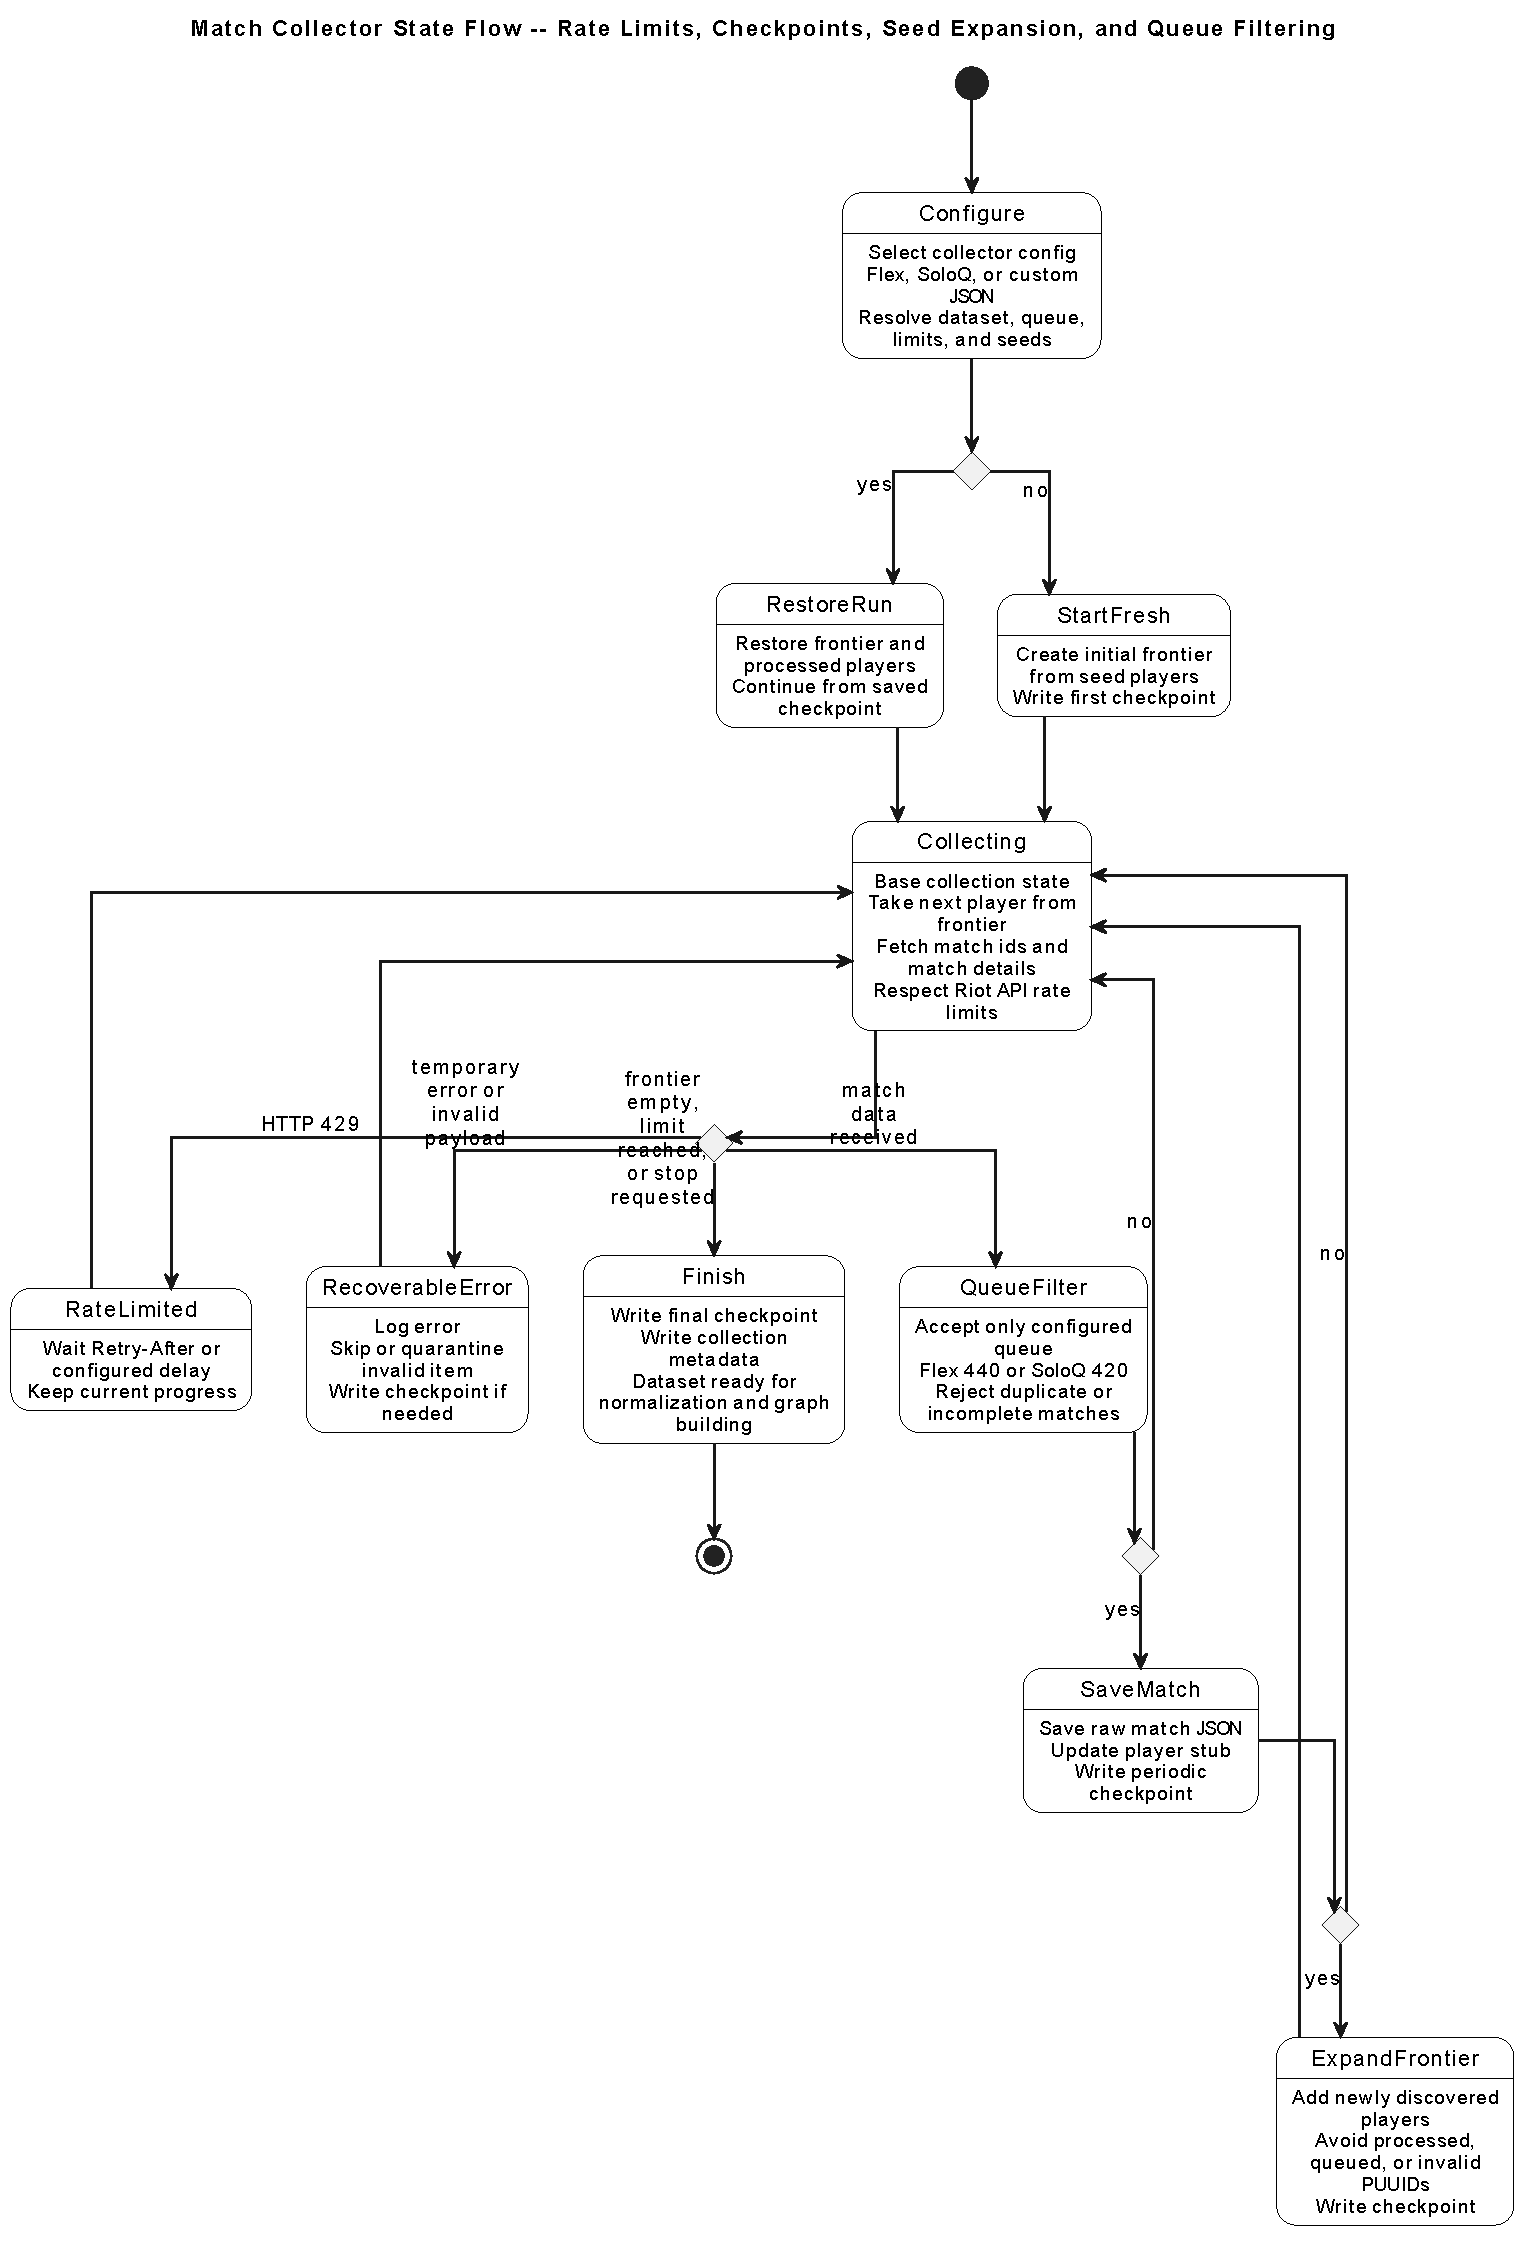
\includegraphics[width=0.98\textwidth,height=0.74\textheight,keepaspectratio]{collector-state-machine.pdf}
\caption{A collector paraméterezhető állapotgépének folyamatábrája}
\end{figure}

\section{Gyűjtési fókusz és queue-választás}

A projekt két kutatási datasetet használ: a \textit{flexset} Ranked Flex Queue meccsekből áll, a \textit{soloq} Ranked Solo/Duo Queue meccsekből. A korai fejlesztési fázisban keletkezett \textit{default} dataset vegyes összetételű (Ranked Flex, Ranked Solo/Duo, ARAM, normál draft és egyéb queue-k keverednek benne), ezért kutatási célra nem alkalmas. Az aktív elemzések kizárólag a \textit{flexset} és \textit{soloq} datasetekre támaszkodnak, amelyek célzott és reprodukálható stratégiával épültek fel.

A queue-típus megválasztása nem tetszőleges. A Ranked Flex megengedi a premade csapatok részvételét, ezért a visszatérő szövetségesi kapcsolatok természetes módon jelenhetnek meg. A Ranked Solo/Duo szándékosan kizárja az 5-fős premade-et, így kontrollált összehasonlítási alapként szolgál. Ez a kettősség az empirikus fejezetek értelmezési keretét is megadja.

\section{Premade-fókusz és gyűjtési stratégiai intuíció}

A projekt mögött végig ott állt az a gyakorlati intuíció, hogy az igazán érdekes kapcsolatok nem az egyszeri, véletlenszerű találkozásokból születnek, hanem a visszatérő együtt- vagy egymás ellen játszásból. Emiatt a gyűjtőszkriptek és a dokumentáció egy része kifejezetten premade-szerű vagy ismétlődő kapcsolatok felderítésére van hangolva.

Ez a szemlélet a teljes későbbi rendszerre hatással volt:

\begin{itemize}
    \item a gráfépítésben élküszöb jelent meg;
    \item az analitikák az ismétlődő kapcsolatokat tekintik komoly jelöltnek;
    \item a pathfinder-költségek is a kapcsolaterősséget veszik figyelembe.
\end{itemize}

Másképp fogalmazva: a gyűjtési stratégia nem előszoba, hanem a gráfjelentés egyik meghatározó forrása.

Ez a döntés ugyanakkor tudatos torzítást is bevezet. Ha a gyűjtés a visszatérő, premade-szerű kapcsolatokat részesíti előnyben, akkor a korpusz kevésbé reprezentálja az egyszeri és lazább találkozásokat. A jelen dolgozat céljai mellett ez elfogadható kompromisszum, mert a kutatási kérdés középpontjában éppen a tartósabb kapcsolati magok állnak. A háló tehát nem a teljes populáció semleges lenyomata, hanem az ismétlődő interakciók felé célzottan dúsított részvilág.

\section{Rate limit, megbízhatóság és operatív kompromisszumok}

A Riot API használata az architektúrában nem pusztán külső függőség, hanem korlátozó tényező is. A fejlesztői kulcsok lekérdezésszámhoz kötöttek, ezért a gyűjtőrétegben explicit sebességkorlát-kezelés, várakozási logika és részfeladatokra bontás jelent meg. A dokumentációban rögzített rate-limit elemzés ezt nem adminisztratív részletként, hanem rendszertervezési kényszerként kezeli.

Ennek közvetlen következményei:

\begin{itemize}
    \item a meccsletöltés nem kérésenkénti frontend-akcióként, hanem háttérfolyamatként fut;
    \item a nyers adatállapotot érdemes lokálisan cache-elni;
    \item a grafikus és analitikai oldal nem függhet attól, hogy egy élő API-lekérés éppen sikeres-e.
\end{itemize}

Ez a döntés később az egész rendszer egyik alapelve lett: \emph{a demo- és kutatási réteg a már összegyűjtött korpuszra épül, nem online API-kérésekre}.

Az implementáció szintjén ez több konkrét védelmet jelent. A collector saját másodpercenkénti várakozást alkalmaz, külön kétperces ablakban számlálja a kéréseket, HTTP 429 esetén harminc másodpercet vár, majd újrapróbálkozik, és a már elmentett meccseket fájllétezés alapján kihagyja. Ez a működés idempotenssé teszi a letöltést: egy megszakadt vagy újraindított futás nem írja felül feleslegesen a korábbi állományokat, és nem épít újabb bizonytalanságot a nyers korpuszba.

\begin{table}[H]
\centering
\caption{A collector fő megbízhatósági mechanizmusai}
\begin{tabularx}{\textwidth}{>{\raggedright\arraybackslash}p{4.4cm}|X}
\toprule
\textbf{Mechanizmus} & \textbf{Funkció} \\
\midrule
Másodpercenkénti késleltetés & A rövid távú API-terhelés kontrollja \\
Kétperces számláló & Illeszkedés a Riot kulcshasználati limitjeihez \\
429 újrapróbálás & Robusztusabb működés átmeneti limitütközéskor \\
Létező meccsfájl kihagyása & Duplikált mentés és újra-letöltés elkerülése \\
Eseményes stdout log & Backend- és frontend-oldali állapotkövetés támogatása \\
\bottomrule
\end{tabularx}
\end{table}

Ezek a döntések nem puszta üzemeltetési kényelmi funkciók. A reprodukálható számítógépes kutatás egyik alapelve, hogy az eredményekhez vezető lépések nyomon követhetők és lehetőleg automatizálhatók legyenek \cite{sandve2013}. A collector parametrizálhatósága, eseményes logolása és idempotens mentési logikája pontosan ezt a célt szolgálja.

\section{A flexset és a soloq gyűjtési stratégiájának összehasonlítása}

A \textit{flexset} dataset kizárólag 440-es queue ID-jű (Ranked Flex) meccseket tartalmaz, EUNE Master$+$ ranglista-pozíciójú seed-játékosoktól. A collector premade-probe mechanizmusa kiszűri azokat a jelölteket, akiknek nincs elegendő visszatérő csapattársi mintázatuk; a befogadottakat csapattársaik azonosítói alapján bővíti tovább (snowball sampling). Az eredmény közel 4980 meccs, erősen összefüggő, visszatérő kapcsolatokban gazdag háló.

A \textit{soloq} dataset 420-as queue ID-jű (Ranked Solo/Duo) meccsekből áll, EUNE Master$+$ Solo/Duo ranglistás seed-populációval. Ez nem azonos a \textit{flexset} seed-populációjával: a Flex Queue és a Solo/Duo Queue ranglistái eltérő mechanikán alapulnak, és más játékosbázist fednek le. A probe-logika itt nem szűr premade-jelenlét alapján, a corpus körülbelül 2000 meccsel zárul. A \textit{soloq} szerepe kontrollalap: olyan dataset, ahol a visszatérő premade-kapcsolatok szisztematikusan nem favorizáltak, ezért a két dataset összehasonlítása megalapozottabb.

\begin{table}[H]
\centering
\caption{A két dataset gyűjtési stratégiájának összehasonlítása}
\begin{tabularx}{\textwidth}{>{\raggedright\arraybackslash}p{4.2cm}|X|X}
\toprule
\textbf{Dimenzió} & \textbf{flexset} & \textbf{soloq} \\
\midrule
Queue ID & 440 (Flex) & 420 (Solo/Duo) \\
Premade-probe & Igen, ismétlések alapján & Nem \\
Seed-terjeszkedés & Csapattársak alapján & Listalekéréssel \\
Gyűjtési cél & Szociális struktúra & Teljesítmény-alapvonal \\
Corpus mérete & 4980 meccs & 2000 meccs \\
Szerep a projektben & Fő kutatási adatkészlet & Kontroll-adatkészlet \\
\bottomrule
\end{tabularx}
\end{table}

Mindkét dataset gyűjtése leáll, ha elérte a konfigurált meccsszám- vagy iterációs limitet, a gyűjtési sor kiürült, vagy manuálisan le lett állítva. A nyers meccs-JSON fájlok fájlrendszeren perzisztálódnak; az idempotens fájlellenőrzés garantálja, hogy már letöltött meccsek nem kerülnek újra letöltésre.

\section{Adatminőség, torzítás és óvatos interpretáció}

A Riot API formálisan pontos, de a dolgozat szempontjából az adat így sem „semleges". A mintavételt erősen befolyásolja, hogy milyen seed játékosokról indult a gyűjtés, mely queue-k kerültek előtérbe, milyen mélyre ment a meccslista-lekérés, és a premade-kapcsolatok milyen minimumismétlés után tekinthetők érdekesnek.

Ezért a dolgozat minden későbbi eredményénél fontos megjegyzés, hogy a hálózat \emph{nem a teljes League of Legends univerzum reprezentációja}, hanem egy adott gyűjtési stratégia által létrehozott, vizsgálható részvilág. Ez nem gyengeség, hanem korrekt keretfeltétel.

További torzításforrás, hogy a dataset fokozatosan épülő archívumként működik. A meccsek nem egyetlen, szigorúan lezárt időablakból származnak, ezért a játékosok \textit{match\_count} értékei részben azt is tükrözik, mennyire került rájuk fókusz a gyűjtési folyamatban. Emiatt a score-réteg és az időbeliség kapcsolatát mindig óvatosan kell kezelni: a magasabb mintaszám nem kizárólag aktivitást, hanem gyűjtési figyelmet is jelenthet.

\chapter{A rendszer korai változata és az eredeti pipeline}

\section{A korai projekt jellege}

A repository története alapján a rendszer első változata jóval közelebb állt egy adatvezérelt játékosnézőhöz és kísérleti gráf-exportáló eszközhöz, mint a jelenlegi, több rétegre bontott kutatási platformhoz. Ebben a szakaszban a cél elsősorban az volt, hogy:

\begin{itemize}
    \item a Riot API-ból érkező nyers mérkőzésadatok egy helyre kerüljenek;
    \item a játékosokhoz legalább alapvető pontszámok rendelődjenek;
    \item a kapcsolatokból egyszerű gráf és klaszterkimenet szülessen;
    \item a projekt vizuálisan is megmutatható legyen.
\end{itemize}

Ez a korai szakasz nem eldobandó előtörténet, hanem a jelenlegi rendszer kiindulópontja. A dolgozatban azért tartom meg hangsúlyosan, mert ebből érthető meg, miért alakult ki később a többnyelvű architektúra és a szigorúbb perzisztenciamodell.

\section{Az első pontozási logika}

Az eredeti \texttt{add\_new\_players.js} egyszerűbb, kézzel összeállított képletekkel dolgozott. A korai \texttt{feedscore} lényegében a halálokat büntette a kill és assist mennyiségéhez képest, míg az első \texttt{opscore} főként a következő komponensekre támaszkodott:

\begin{itemize}
    \item ölések,
    \item asszisztok,
    \item arany,
    \item vision score.
\end{itemize}

Ez a kezdeti modell nyers volt, de fontos előnye volt: gyorsan megmutatta, hogy a tiszta KDA-logikán túl is lehet értelmes, legalább részben kompozit teljesítménymutatót számolni. Később ebből nőtt ki az artifact-szintű és szerepkörérzékeny rendszer.

\section{A korai gráfépítés és export}

A korai \texttt{build\_graph.py} és a hozzá kapcsolódó exportlépések alapvetően Python-központúak voltak. A hangsúly ekkor még a gyors láthatóságon és nem a perzisztens újrafelhasználhatóságon volt. A pipeline:

\begin{itemize}
    \item meccsekből kapcsolati gráfot épített,
    \item összefüggő komponenseket és részgráfokat vizsgált,
    \item HTML és PyVis exportokat készített,
    \item gyors vizuális ellenőrzést tett lehetővé.
\end{itemize}

Ez a megközelítés jó prototípus volt, de rövid időn belül látszott a korlátja: a klaszterek és gráfnézetek csak exportként éltek tovább, és nem váltak a rendszer belső, lekérdezhető objektumaivá.

\section{A korábbi régiós és ország-alapú ág kialakulása}

A projekt korai időszakában erősebb szerepet kapott az a gondolat is, hogy a klaszterekből ország- vagy régiószintű következtetések szülessenek. Ennek nyomai ma is megtalálhatók a \texttt{fetch\_clusters.py}, \texttt{assign\_countries.py} és \texttt{conclude.py} szkriptekben. A megközelítés lényege az volt, hogy a klaszterek tagneveiből valamilyen földrajzi címke becsülhető, majd ehhez aggregált teljesítményadatok rendelhetők.

Ez a gondolat önmagában izgalmas, de a dolgozat mostani állapotában már világos, hogy módszertanilag bizonytalanabb, mint a közvetlenül a gráfstruktúrára és a meccsadatokra támaszkodó elemzések. Emiatt ezt a vonalat nem törlöm ki a történetből, hanem kifejezetten korábbi, exploratív modulként kezelem.

\section{Miért kellett a rendszert továbbépíteni?}

A korai változat legfontosabb korlátai a következők voltak:

\begin{itemize}
    \item egyetlen adatbázis és egyetlen meccskönyvtár köré szerveződött;
    \item a klaszterek és exportok nem voltak igazán első osztályú perzisztens objektumok;
    \item a pontozás még nem volt kellően szerepkörérzékeny;
    \item a futásidejű útvonalkeresés és a nehezebb gráfanalitika nem vált el élesen a frontend-logikától.
\end{itemize}

Ezek a hiányok nem kudarcot jeleztek, hanem természetes érési pontokat. A jelenlegi rendszer legjobban akkor érthető, ha nem egyetlen pillanatfelvételként, hanem ilyen fokozatos evolúció eredményeként nézzük.

Visszatekintve a projekt korai szakaszának legtermészetesebb csapdája az \emph{akkumulatív script-architectúra} lett volna, amelyben minden új feature egy újabb script formájában kerül be, és az egész rendszer globális állapottól függ. Ez a minta sok hasonló méretű adat-kutatási projektben megfigyelhető. Azzal, hogy a projekt tudatosan bevezette a dataset-absztrakciót, a Rust-szintű analitikai elválasztást és a perzisztens klasztermodellt, elkerülte ezt a csapdát.

Döntő fordulópontot jelentett az a felismerés, hogy \emph{a kutatási analitikának nem szabad a frontend-állapottól függenie}. Ha az asszortativitás kiszámítása frontend-kérésre, a böngészőben lévő adatokból történne, akkor egyrészt nem lenne reprodukálható, másrészt nagyon érzékeny lenne a felhasználói interakcióra. A Rust-oldali, parancssori futtathatóság ezt a problémát gyökeresen oldja meg.

\section{Miért kellett a régi szövegréteget is megtartani?}

Szakdolgozatírás közben könnyű lenne azt a hibát elkövetni, hogy a projekt korábbi állapotát egyszerűen ``lecserélem'' a jelenlegi, erősebb verzióra. Ezt tudatosan nem teszem. A korai pipeline, a \texttt{conclude.py}-szerű ág és a régi klaszterértelmezések azért maradnak a dolgozatban, mert ezek adják meg a fejlődés irányát. A mostani rendszer nem légüres térben született, hanem ezekből nőtt ki.

A country-alapú ágat (a \texttt{assign\_countries.py} és a \texttt{conclude.py} modulokat) jelenleg elavultnak tekintem: az ország-hozzárendelés megbízhatósága nem elegendő ahhoz, hogy a projekt fő állításait erre épüljenek, és a kód aktív karbantartás nélkül is a repositoryban marad mint történeti dokumentum. Ugyanakkor az a gondolat, hogy a klasztereket értelmezési egységként kezeljük - és ne csak vizuális exportként -, ebből az ágból nőtt ki. Ebben az értelemben az ott szerzett tapasztalat a jelenlegi klasztermodel egyik alapköve.

\diagramfigure{A korai Python-alapú adatgyűjtő és gráfépítő pipeline adatáramlása}{old python graph dataflow diagram.pdf}

% Ez a fejezet összevonásra került a 05-ös fejezettel (A rendszer felépítése és evolúciója).

\chapter{Több-adatkészletes architektúra}

\section{Miért vált szükségessé a dataset-regiszter?}

Az egyetlen adatbázisos modell korai prototípushoz még elegendő volt, de amint a projekt egyszerre kezdett demo-, smoke-test- és kutatási célokat szolgálni, világossá vált, hogy a különböző minták szétválasztása nélkül a rendszer nehezen reprodukálható. Ugyanaz a frontend, ugyanaz a Rust futtatókörnyezet és ugyanaz a Python pipeline más eredményt adhat, ha eltérő bemeneti korpuszon fut. Ezt a különbséget nem rejtett konfigurációs fájlokban, hanem explicit dataset-regiszterben érdemes kezelni.

A dataset-regiszter bevezetésének szükségességét konkrét igényváltozás indokolta:

\begin{itemize}
    \item \textbf{Smoke-teszt igény}: a fejlesztői pipeline-t kis adathalmazzal kell tudni validálni, anélkül hogy az éles adatbázist módosítani kellene;
    \item \textbf{Kutatási szétválasztás}: a Flex Queue és a Solo/Duo Queue strukturálisan eltérő gráfot hoz létre; az eredmények összekeveredése módszertanilag hibás lenne;
    \item \textbf{Reprodukálhatósági garancia}: ha a fő kutatási dataset változik, a régi dataset-állapot is ellenőrizhető maradjon;
    \item \textbf{Pipeline-átjárhatóság}: a Rust analitika, a Python klaszterpipeline és a Node/Express API mind ugyanarra a dataset-re álljon rá, ne legyen ``backend igazság'' és ``Rust igazság'' egymás mellett.
\end{itemize}

Az \textbf{elvetett alternatíva} a konfigurációs fájlon alapuló manuális váltás lett volna: a felhasználó kézzel módosít egy útvonalat, és a rendszer azt használja. Ez nem skálázódik, mert a több állapot egyszerre való megtartása nem lehetséges, és az összekeveredési hibák nehezen detektálhatók.

A \texttt{backend/data/datasets.json} pontosan ezt a feladatot látja el. A dataset fogalma a jelenlegi rendszerben nem csak annyit jelent, hogy ``másik mappa'', hanem egy teljes, együtt mozgó adategységet:

\begin{itemize}
    \item nyers adatbázissal,
    \item finomított adatbázissal,
    \item meccs-JSON könyvtárral,
    \item cache-könyvtárral,
    \item megjeleníthető metaadatokkal.
\end{itemize}

\section{A jelenlegi regiszterben szereplő adatkészletek}

A dolgozat írásakor ellenőrzött \texttt{backend/data/datasets.json} regiszterben négy dataset szerepelt:

\begin{itemize}
    \item \texttt{default} - az eredeti telepítésből migrált, vegyes queue-tartalmú alapkorpusz;
    \item \texttt{smoke-test-dataset} - gyors infrastruktúratesztelésre szánt átmeneti adatkészlet;
    \item \texttt{flexset} - EUNE Master$+$ Flex Queue meccsek, kifejezetten premade és ismétlődő csapattársi kapcsolatok tanulmányozására;
    \item \texttt{soloq} - EUNE Master$+$ Solo/Duo Queue meccsek, kontroll- és teljesítmény-alapvonal-gyűjtés céljából.
\end{itemize}

Az \textbf{aktív dataset a \texttt{soloq}}. Ez a döntés az adatbázis-regiszterben is rögzített: a \texttt{currentDatasetId} mező értéke \texttt{"soloq"}.

A négy dataset jelenléte nem véletlen felhalmozódás, hanem tudatos kutatásstratégia eredménye. A \texttt{default} megőrzi az eredeti, heterogén korpuszt és a korábbi fejlesztési előtörténetet. A \texttt{smoke-test-dataset} a pipeline gyors ellenőrzésére szolgál anélkül, hogy a főadatokat érintené. A \texttt{flexset} és a \texttt{soloq} egymással párban értelmezhetők: az előbbi a premade és csoportos játékhoz kötődő társas jeleket erősíti, az utóbbi pedig ugyanannak a szervernek és rangsornak egyénibb, kevésbé premade-fókuszú meccstörténetét képviseli.

\begin{table}[H]
\centering
\caption{A négy regisztrált dataset összefoglalója}
\begin{tabularx}{\textwidth}{>{\raggedright\arraybackslash}p{3.0cm} >{\raggedright\arraybackslash}p{3.0cm} X}
\toprule
\textbf{Dataset ID} & \textbf{Szerepkör} & \textbf{Jellemzők} \\
\midrule
\texttt{default} & Alap/migrált & Vegyes queue, heterogén tartalom \\
\texttt{smoke-test} & Pipeline-teszt & Átmeneti, infrastruktúra-validálásra \\
\texttt{flexset} & Fő kutatási dataset & EUNE Master$+$ Flex, premade-fókusz \\
\texttt{soloq} & Kontroll/baseline & EUNE Master$+$ Solo/Duo, teljesítmény-alap \\
\bottomrule
\end{tabularx}
\end{table}

A \texttt{flexset} esetében a regiszter metaadata tartalmazza a gyűjtési stratégia dokumentumát és a collector konfigurációs fájl hivatkozását (\texttt{apex\allowbreak-flex\allowbreak-collector.json}). A \texttt{soloq} hasonlóan strukturált: külön collector konfigurációs fájllal és gyűjtési stratégia-dokumentummal rendelkezik. Ez a párhuzamos konfiguráció kifejezetten mutatja, hogy a két dataset nem eseti gyűjtés, hanem tudatosan eltérő stratégiával felépített, összehasonlítható korpusz.

\begin{table}[H]
\centering
\caption{A dataset-regiszter funkcionális szerepei}
\begin{tabularx}{\textwidth}{>{\raggedright\arraybackslash}p{4.2cm}X}
\toprule
\textbf{Funkció} & \textbf{Jelentőség} \\
\midrule
Aktív dataset kijelölése & Meghatározza, hogy a backend és a frontend mely adatkorpuszt használja alapértelmezetten \\
Eltérő tárolási útvonalak & Megakadályozza, hogy a teszt- és főadatok összekeveredjenek \\
Külön cache-ek & A bird's-eye és egyéb előre generált artifaktumok elkülönülnek \\
Kísérleti összevethetőség & Azonos pipeline különböző mintákon is futtatható \\
\bottomrule
\end{tabularx}
\end{table}

\section{A dataset-választás propagálása a backend és a Rust felé}

A dataset-ek architektúrájának egyik legfontosabb technikai előnye az, hogy a választás nem áll meg a Node-szinten. A backend a kiválasztott datasetből környezeti változókat és útvonalakat képez a Rust futtatókörnyezet felé is, például:

\begin{itemize}
    \item \texttt{DATASET\_ID},
    \item \texttt{GRAPH\_DB\_PATH},
    \item \texttt{PATHFINDER\_MATCH\_DIR},
    \item \texttt{PATHFINDER\_BIRDSEYE\_CACHE\_DIR}.
\end{itemize}

Ez építészetileg nagyon fontos döntés. Nincs külön ``frontend igazság'', ``backend igazság'' és ``Rust igazság'' ugyanarról az adatállapotról: a dataset-választás a teljes végrehajtási láncon végigmegy.

A \texttt{server.js} szintjén ez úgy valósul meg, hogy a szerver a kiválasztott datasetből egységes környezeti változókészletet képez, például \texttt{DATASET\_ID}, \texttt{GRAPH\_DB\_PATH}, \texttt{PATHFINDER\_MATCH\_DIR} és \texttt{PATHFINDER\_BIRDSEYE\_CACHE\_DIR} formában. A Rust runtime ezeket fogyasztja, így a teljes végrehajtási lánc ugyanarra az adatvilágra áll rá. Ez lényeges a védhetőség szempontjából: a frontend által mutatott eredmény nem különálló demonstrációs adatból, hanem ugyanabból a datasetből jön, amelyen a kutatási analitika is fut.

\chapter{SQLite perzisztencia és klasztermodellezés}

\section{Miért maradt központi elem az SQLite?}

A projekt mérete és célja szempontjából az SQLite továbbra is kifejezetten jó kompromisszum. Nem igényel külön adatbázisszerver-felügyeletet, könnyen verziózható a séma, gyors a lokális fejlesztésben, és a demo közben sincs szükség külön infrastruktúrára. Ennél is fontosabb, hogy a perzisztens modell egyszerűen ellenőrizhető: a játékos-, klaszter- és tagsági sorok közvetlenül lekérdezhetők.

Egy szakdolgozatban ez külön előny. Nem csak a frontend JSON-kimeneteit lehet megmutatni, hanem az alapul szolgáló relációs tárolást is.

\begin{figure}[H]
\centering
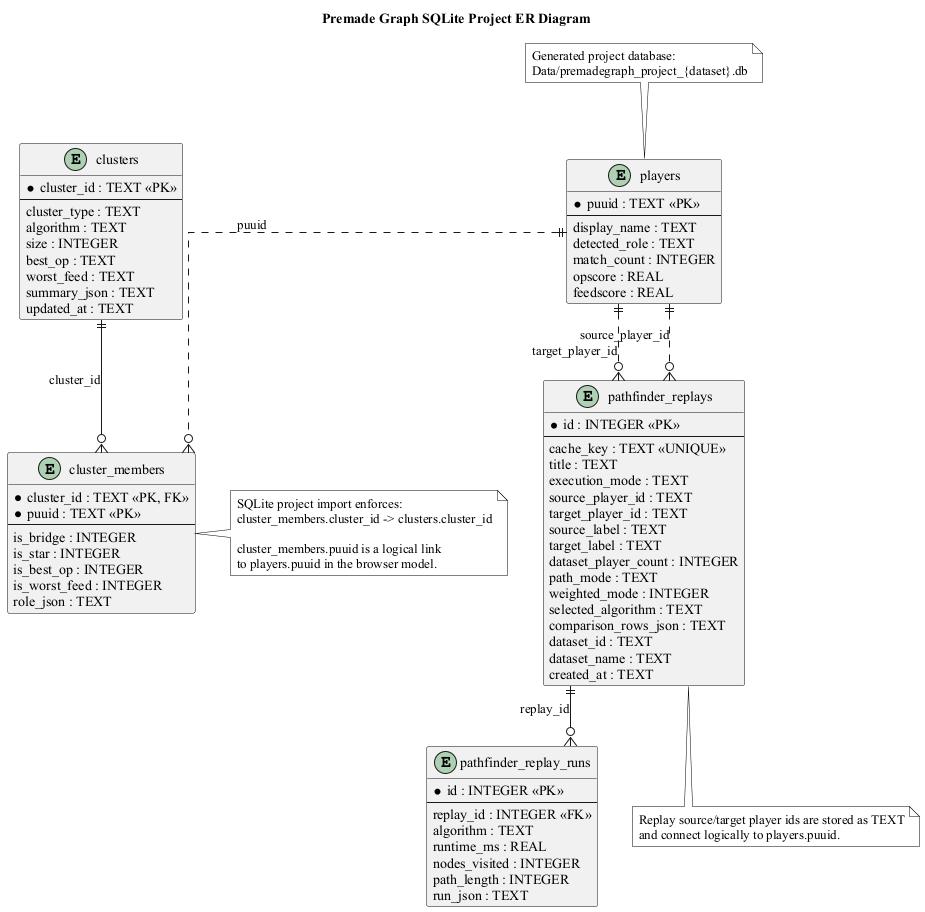
\includegraphics[width=0.98\textwidth,height=0.76\textheight,keepaspectratio]{sqlite-project-er-diagram.png}
\caption{A fő SQLite adatbázis egyedkapcsolati diagramja}
\end{figure}

\section{A \texttt{players} tábla mint gazdagított játékosprofil}

A jelenlegi \texttt{players} tábla már jóval több egy egyszerű névjegyzéknél. A fő mezőcsoportok:

\begin{itemize}
    \item azonosítók és névmezők;
    \item aggregált teljesítménymutatók (\texttt{feedscore}, \texttt{opscore});
    \item mintanagyságot leíró mezők (\texttt{match\_count}, \texttt{matches\_processed});
    \item szerepkör és szerepkör-bizonyosság;
    \item artifact-szintű komponensek.
\end{itemize}

A 2026. április 24-én vizsgált állapotban a tábla \textbf{25\,618} játékost tartalmazott. A szerepkör-eloszlás közel kiegyensúlyozott képet mutatott a fő lane-szerepkörök között, miközben \texttt{UNKNOWN} kategóriába is került \textbf{3120} játékos. Ez a gyakorlatban azt jelenti, hogy a rendszer nem próbál mindenáron erőltetett lane-hozzárendelést végezni ott, ahol a nyers adat nem kellően megbízható.

\begin{table}[H]
\centering
\caption{Szerepkör-eloszlás a vizsgált \texttt{players} állapotban}
\begin{tabular}{lr}
\toprule
\textbf{Szerepkör} & \textbf{Játékosok száma} \\
\midrule
TOP & 4571 \\
MIDDLE & 4517 \\
JUNGLE & 4484 \\
BOTTOM & 4471 \\
UTILITY & 4455 \\
UNKNOWN & 3120 \\
\bottomrule
\end{tabular}
\end{table}

\subsection{Sémanormalizáció és visszafelé kompatibilitás}

A \texttt{backend/normalize\_players\_by\_puuid.js} egyik fontos, de könnyen rejtve maradó tulajdonsága, hogy nem tiszta, egyszer létrehozott sémával számol. A modul deklarálja a \texttt{players} tábla kanonikus oszlopkészletét, és szükség esetén a történetileg felhalmozott eltérésekhez is alkalmazkodik. Ez a projekt evolúciós természetéből következik: a score-réteg, a szerepkörmezők és az artifact-szintű komponensek nem egyszerre, hanem fokozatosan kerültek be a modellbe.

Ennek szakdolgozati jelentősége is van. A rendszer nem laboratóriumi körülmények között egyszer megtervezett és lezárt adatbázissal dolgozik, hanem olyan struktúrával, amely a fejlesztés közben bővült. A normalizáló modul ezért egyben migrációs réteg is: megőrzi a régebbi állapotok használhatóságát, miközben előkészíti az újabb analitikai mezőket.

\subsection{SQLite pragmák és írási kompromisszumok}

A normalizáló pipeline az SQLite-ot nem alapbeállításokkal használja. A kód explicit módon \texttt{WAL} naplózást, \texttt{NORMAL} szinkronizációt, memóriabeli ideiglenes tárolást és foreign key támogatást állít be. Ez a választás jól mutatja, hogy az SQLite jelenléte nem „egyszerűségi lustaság”, hanem tudatos kompromisszum. A rendszernek lokálisan futó, ismételten újraíró, de nem többszáz egyidejű felhasználót kiszolgáló analitikai adattárra van szüksége; erre a célra ez a konfiguráció kifejezetten jó arányt ad a sebesség, a stabilitás és a hordozhatóság között.

\section{A klasztermodell és a két fő tábla szerepe}

A klaszterek perzisztenciáját a \texttt{clusters} és \texttt{cluster\_members} páros adja. A \texttt{clusters} tábla főbb elemei:

\begin{itemize}
    \item \texttt{cluster\_id},
    \item \texttt{cluster\_type},
    \item \texttt{algorithm},
    \item \texttt{size},
    \item \texttt{summary\_json},
    \item térbeli koordináták,
    \item build-verzió és frissítési idő.
\end{itemize}

A \texttt{cluster\_members} tábla ezzel szemben tagsági és szerepkörjellegű információt tárol:

\begin{itemize}
    \item a klaszter és játékos összerendelését;
    \item \texttt{is\_bridge}, \texttt{is\_star}, \texttt{is\_best\_op}, \texttt{is\_worst\_feed} jelzőket;
    \item szerepköri összegzést \texttt{role\_json} formában.
\end{itemize}

Ez a modell azért erős, mert a klaszter nem puszta név vagy címke, hanem lekérdezhető objektum, amelyhez külön metaadatok és tagsági szerepek kötődnek.

A \texttt{backend/cluster\_persistence.py} további fontos döntése, hogy a klaszterek cseréjét \texttt{cluster\_type} szerint végzi. Vagyis egy új \texttt{python\_population} build felülírja a régi Python-klasztereket, de nem nyúl a \texttt{rust\_pathfinding} családhoz. A művelet előbb törli az adott típushoz tartozó régi tagsági sorokat, majd a klasztermetaadatokat, és ezután írja be az új eredményt. Ez a szemantika nagyon hasznos, mert ugyanazon adatbázisban több klasztercsalád élhet együtt anélkül, hogy egy újrafuttatás mindent elsöpörne.

A \texttt{summary\_json}, \texttt{role\_json}, \texttt{build\_version} és \texttt{updated\_at} mezők a kutatási visszakövethetőséget is javítják. A klaszter így nem pusztán tagsági halmaz, hanem olyan objektum, amelynek eredete, típusa és részleges összefoglaló állapota is megmarad.

\section{A perzisztált klaszterek aktuális nagyságrendje}

A két fő kutatási dataset finomított adatbázisainak ellenőrzött állapota alapján a klaszterstruktúra lényegesen eltér a két korpuszban:

\textbf{Flexset} (\texttt{playersrefined.db}):
\begin{itemize}
    \item \textbf{599} klaszter a \texttt{clusters} táblában;
    \item \textbf{5741} klasztertagsági rekord a \texttt{cluster\_members} táblában;
    \item a Graph V2 artfaktumban \textbf{1531} látható klaszter, átlagos méret \textbf{3.750}, legnagyobb \textbf{20}.
\end{itemize}

\textbf{SoloQ} (\texttt{playersrefined.db}):
\begin{itemize}
    \item \textbf{140} klaszter a \texttt{clusters} táblában;
    \item \textbf{1538} klasztertagsági rekord a \texttt{cluster\_members} táblában;
    \item a Graph V2 artfaktumban \textbf{870} látható klaszter, átlagos méret \textbf{1.768}, legnagyobb \textbf{20}.
\end{itemize}

A két szám közötti különbség metodikailag fontos. A \texttt{clusters} táblában tárolt klaszterek a Python pipeline által meghatározott, populációs alapú közösségek. A Graph V2 látható klasztereinek száma magasabb, mert a Graph V2 külön, kötetlen ally-csoportként kezeli azokat a csomópontokat is, amelyek csak vizualizációs szempontból alkotnak csoportot. A flexset lényegesen sűrűbb klaszterstruktúrát mutat: az átlagos klaszterméret (3.750) a soloq-hoz képest (1.768) közel duplája, ami empirikusan is alátámasztja, hogy a Flex Queue erősebb ismétlődő csoportkapcsolatokat termel.

Ez önmagában is fontos rendszerszintű eredmény, mert mutatja, hogy a többdataset-architektúra valódi különbséget fog meg, nem csupán méretbeli eltérést.

\section{A két klasztercsalád részletes összehasonlítása}

A rendszerben két klasztercsalád él párhuzamosan, amelyek különböző módszerrel és célra épülnek:

\subsection{python\_population}

A \texttt{python\_population} típusú klaszterek a korai Python gráfépítési pipeline kimenetei. Ezeket a \texttt{backend/build\_graph.py} jellegű modulok és NetworkX-alapú modularitási közösségdetektálás hozzák létre a nyers meccsadatok alapján. Főbb jellemzők:

\begin{itemize}
    \item a klaszterméret nincs kemény korláthoz kötve (a moduláris detektálás saját maga dönt a méretekről);
    \item az algoritmus a globális moduláris optimalizáció szempontjából határozza meg a csoportokat;
    \item a flexset dataseten például közepes méretű, $\sim$10--15 fős klaszterek is keletkezhetnek, ha a moduláris struktúra azt indokolja;
    \item a Python klaszterek inkább \emph{közösségdetektálási} perspektívát tükröznek.
\end{itemize}

\subsection{rust\_pathfinding}

A \texttt{rust\_pathfinding} típusú klaszterek a Rust motor futásidejű klaszterezési logikájából jönnek. Az implementáció az ally-kapcsolatokon alapuló erős-összefüggési szegmensekre bontja a gráfot, kemény méretkorláttal (maximum 20 tag). Főbb jellemzők:

\begin{itemize}
    \item a 20 tagos korlát garantálja a klaszterek áttekinthetőségét a frontend vizualizációban;
    \item az oversized összefüggő komponensek determinisztikusan kerülnek szétvágásra;
    \item a Rust klaszterek főként \emph{pathfinding és vizualizációs} célra optimalizáltak;
    \item az \texttt{orbitScore} és \texttt{orbitRadius} értékek kizárólag a Rust klaszterekre értelmezhetők.
\end{itemize}

\subsection{A két csomád koegzisztenciájának módszertani értéke}

A két klasztercsalád nem egymást helyettesíti, hanem egymást kiegészíti. A Python klaszterek adnak egy moduláris alapú közösségstruktúrát; a Rust klaszterek ennek futásidejű, vizualizáció-kompatibilis változatát. Az a tény, hogy mindkét klaszter-nézet egyszerre létezik az adatbázisban, lehetővé teszi, hogy például az asszortativitási bontásoknál explicit módon megkérdezhetjük: a Python-közösségek belső éleire vagy a Rust-vizualizációs csoportok belső éleire mért asszortativitás-e erősebb?

\section{Miért fontos a perzisztencia a kutatási fejezetekhez?}

Az asszortativitási, központisági és kísérleti signed-balance számítások látszólag a Rust oldalon történnek, de valójában a korábban kialakított perzisztens modell nélkül sokkal nehezebben lennének értelmezhetők. A klaszterekhez kötött bontások, a játékosprofilokhoz rendelt score-ok és a későbbi exportok mind arra támaszkodnak, hogy a játékos és a közösségi kontextus ugyanabban a perzisztens rendszerben elérhető.

Ez jó példa arra, hogy az adatbázistervezés nem csak kiszolgáló infrastruktúra, hanem a kutatási érték egyik feltétele.

\chapter{Az opscore teljesítménymetrika}

\section{Gyűjtési stratégia}

A projekt adatgyűjtő rétege a Riot API-ra épül. A jelenlegi architektúrában a meccsek begyűjtése nem egyetlen frontend gombnyomásra történő monolitikus folyamat, hanem paraméterezhető háttérfeladat, amely a datasethez kötve fut. A backend oldalon a gyűjtéshez tartozik:

\begin{itemize}
    \item aktív dataset kiválasztása,
    \item lekérdezési limit figyelembevétele,
    \item iterációszám és meccsszám paraméterezése,
    \item queue-típus szerinti szűrés,
    \item véletlen vagy konkrét játékos-alapú indítás.
\end{itemize}

A Riot API korlátai mellett csak olyan rendszer tartható karban hosszabb távon, amely a gyűjtést külön modulnak tekinti, és nem keveri össze a futási idejű vizualizációval.

\section{Normalizálás PUUID alapján}

A nyers adatok összefűzésének kulcsa a \texttt{puuid} alapú normalizálás. A játékosnevek változhatnak, a különböző meccsekben eltérő formában is megjelenhetnek, ezért a rendszer az egyedi azonosítót tekinti az elsődleges kulcsnak. A normalizálás során a pipeline:

\begin{itemize}
    \item végigolvassa a meccs-JSON fájlokat,
    \item résztvevőnként kinyeri a releváns mezőket,
    \item szerepkört rendel a \texttt{teamPosition} alapján,
    \item meccsszintű artifactokat számol,
    \item játékosszinten átlagol és normalizál,
    \item a végeredményt a \texttt{players} táblába írja vissza.
\end{itemize}

Ez adja a rendszer egyik központi alapját, mert minden későbbi gráfanalitika erre a normalizált játékosprofilra támaszkodik.

\section{A teljesítménymetrika szükségessége}

A gráfanalitikai elemzés alapanyagát egy értelmes, szerepkörérzékeny teljesítménypontszám jelenti. A League of Legends meccsek nyers adatai (ölések, halálok, arany, sebzés) önmagukban nem hordoznak elegendő szemantikát: egy support 2 halála nem ugyanolyan értelmű, mint egy ADC 2 halála, egy jungler alacsony CS-értéke nem büntetendő ugyanúgy, mint egy laneré, és egy split-pusher alacsony csapaterősítő statisztikái nem feltétlenül jelzik gyenge meccsteljesítményt. Ahhoz, hogy a játékosokat egy gráfban összehasonlítható csúcsokként lehessen kezelni, szükség van egy olyan mutatóra, amely a meccsstatisztikákat szerepkör-specifikus elvárások alapján értelmezi.

Az \texttt{opscore} célja ezért nem az, hogy abszolút igazságmértékként funkcionáljon, hanem az, hogy egy következetes, értelmezhető és módszertanilag védhető skálát hozzon létre. Ez a skála az asszortativitási elemzés, a centralitásvizsgálat és az esetleges szimulációs seeding alapjaként szolgál. A metrika akkor tekinthető hasznosnak, ha különböző játékosokhoz és különböző meccsekhez következetesen rendel értelmes értékeket, függetlenül attól, hogy az aktuális adatbázis éppen erős vagy gyenge játékosokból áll.

\section{A korábbi modell módszertani korlátai}

A modell fejlesztése fokozatos módszertani finomítás eredménye volt. A kiindulópontot egy nyolc-artifactos rendszer adta, amely szerepkör-szorzókat alkalmazott, majd a kapott nyers összegeket az adatbázis percentilis-eloszlásához viszonyítva normalizálta a $[0,10]$ tartományra. Ebben a korábbi modellben az eredmény három horgonyhoz igazodott: az 5.~percentilishez, a mediánhoz és a 95.~percentilishez; a medián játékos körülbelül $6{,}6$-os értékre esett.

Bár ez a megközelítés működőképes volt, két alapvető gyengeség hamar felszínre került.

\paragraph{Adatbázis-relatív normalizálás.}
Ha az adatbázis túlnyomórészt nagyon erős játékosokat tartalmaz, a medián játékos is a skála közepe körüli értéket kap, hiába teljesít objektív szempontból kiemelkedően. Fordítva: ha az adatbázis viszonylag gyengébb játékosokból áll, ugyanaz a mediánteljesítmény szintén a skála közepén jelenik meg. Egy Challenger-szintű dataseten belüli medián és egy Bronze-szintű dataseten belüli medián numerikusan közel eshet egymáshoz. Ez azonban nem teljesítményállítás, csupán adatbázis-relatív elhelyezkedés. A gráfanalitika szempontjából ez különösen problematikus, mert az asszortativitás és a centralitás értelmezéséhez stabil, adatbázisfüggetlen teljesítménycímkékre van szükség.

\paragraph{A korábbi halálokon alapuló közelítés korlátai.}
A korábbi rendszer a halálokat és a kill-participationt egy külön, szándékosan minimális formulával értékelte, amely a halálokat büntette, a kill-participationt engedményként kezelte. Ez a közelítés azonban nem tudott különbséget tenni az alábbi, szemantikailag eltérő szituációk között:
\begin{itemize}
    \item egy tank, amely csapattársi nyomást vesz magára és ezzel lehetővé teszi a csapat manőverét;
    \item egy support, aki helyes engage-beállítás közben hal meg;
    \item egy split-pusher, aki szándékosan kerüli a csatatereket, de struktúrákon keresztül nyeri a meccset;
    \item egy carry, aki a meccs eldöntése után hal meg a késői fázisban;
    \item és egy ténylegesen alacsony értékű feeder, aki ismételten tempót ajándékoz az ellenfeleknek.
\end{itemize}
A korábbi képlet ezeket az eseteket nem tudta megkülönböztetni, mert nem vette figyelembe a meccs hosszát, a halálok eltöltött idejét, a szerepköri elvárásokat, a csapaterőhöz való viszonyt, vagy azt, hogy a halálokat ellensúlyozta-e valamilyen win condition-beváltás. Ez módszertani gyengeség, amelyet a jelenlegi modell strukturálisan orvosol.

Egy harmadik korlát az volt, hogy a korábbi rendszerben az artifactok értékét egy merev felső korlát szorította: minden artifact maximális hozzájárulása közel azonos volt. Ez elfedte az elité, win-condition-szintű teljesítményeket, például egy extrém KDA-val rendelkező carry meccset, amelyet a korábbi modell középszerű értékre komprimálhatott.

\section{A helyi, szerepkörérzékeny opscore modell}

A jelenlegi \texttt{opscore} modell ezeket a korlátokat a következő tervezési elvek mentén kezeli.

\paragraph{Lokális, adatbázis-független értékelés.}
Az értékelés alapja a szerepkör-specifikus elvárás, nem az aktuális adatbázis eloszlása. Egy meccs teljesítménye értékelhető közvetlenül a meccsen belüli kontextusból, anélkül, hogy tudni kellene, kik is vannak jelen az adatbázisban. Az adatbázis-átlagok továbbra is hasznosak diagnosztikai összehasonlításra, de nem határozzák meg a jegyet.

\paragraph{Öt artifact, tíz alkategória.}
A teljesítményt öt értelmező artifact fogja át, amelyek mindegyike két alkategóriára bontódik. Ez a szerkezet elég részletes ahhoz, hogy különböző playstyle-okat megkülönböztessen, de elég átlátható ahhoz, hogy a végeredmény értelmezhetőségét megőrizze.

\paragraph{Logaritmikus bővítés elité teljesítményeknél.}
Az artifactokhoz nominális $[0, 2]$ ponttartomány tartozik, de kivételes teljesítmény esetén ez a korlát kontrolláltan átléphető. Csak a végső \texttt{opscore} van keményen korlátozva $10$-re.

\paragraph{Rövid meccsek megbízhatósági kezelése.}
A percenkénti mutatók labilis becslők rövid meccsekben. A modell egy megbízhatósági szorzóval simítja el a rövid meccsek outlier értékeit, ezáltal megelőzve, hogy egy 15 perces korai megadás irreális szélső pontszámot eredményezzen.

Az implementáció a \texttt{backend/scoring\_config.js}, a \texttt{backend/lib/scoring\_utils.js} és a \texttt{backend/normalize\_players\_by\_puuid.js} fájlokban van rögzítve.

\section{Az öt artifact és alkategóriáik}

\begin{figure}[H]
\centering
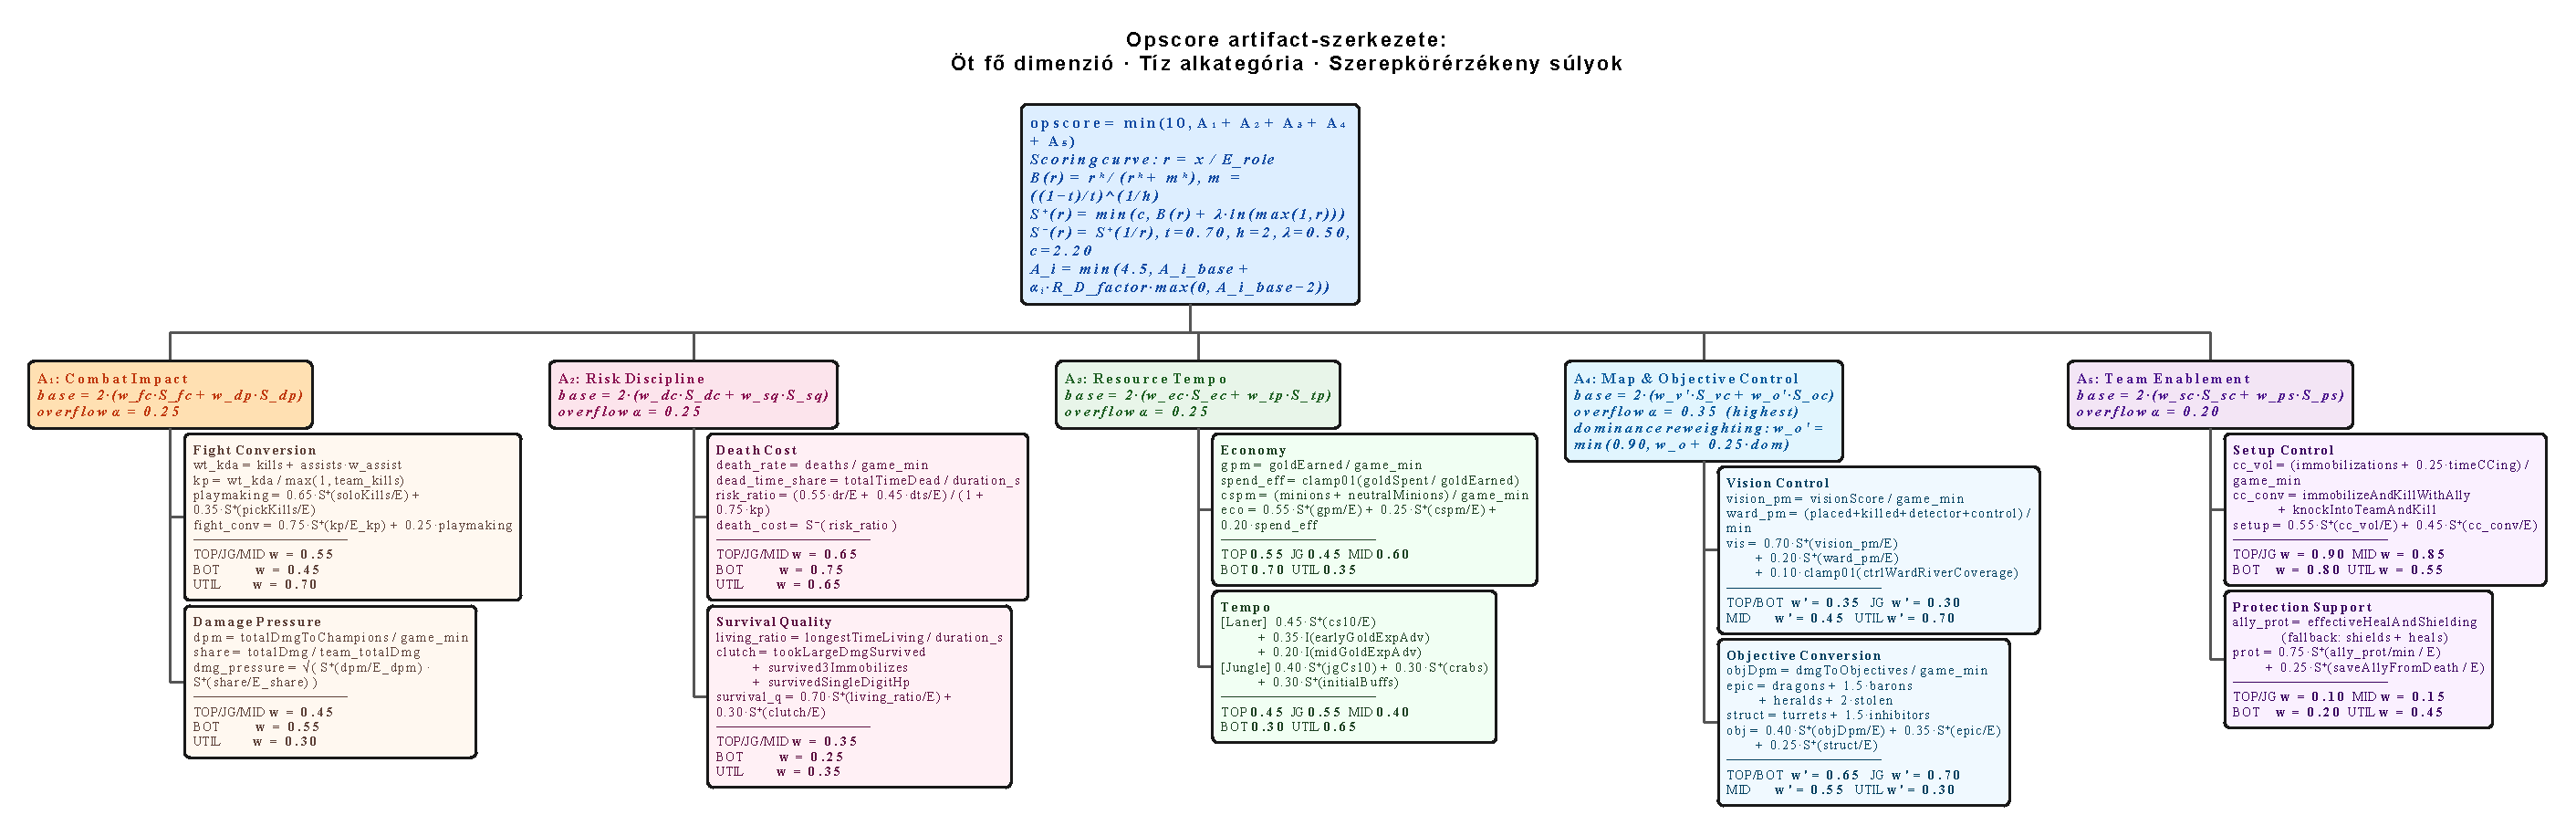
\includegraphics[width=0.98\textwidth,height=0.76\textheight,keepaspectratio]{opscore-artifacts.pdf}
\caption{Az opscore artifact-szerkezete: öt fő dimenzió, tíz alkategória, szerepkörérzékeny súlyok}
\end{figure}

A modell öt artifactból épül fel. Minden artifact két alkategóriából áll, amelyek szerepkörönként eltérő súllyal járulnak hozzá az artifact értékéhez.

\subsection{\texttt{Combat Impact}}

A \texttt{Combat Impact} artifact azt méri, hogy a játékos mennyire hatékonyan konvertálta harcait, és mekkora sebzési nyomást volt képes fenntartani.

Az első alkategória, a \emph{Fight Conversion}, a kill-participation és a csapaterőhöz viszonyított súlyozott takedown-arány alapján értékel. Emellett figyelembe veszi a solo kill és a szövetségessel együtt végrehajtott megölések arányát, mint a harckezdeményezési és döntési képesség mutatóit.

A második alkategória, a \emph{Damage Pressure}, a percenkénti sebzés és a csapaton belüli sebzési arány geometriai közepét veszi alapul. Ez azt jutalmazza, ha a játékos egyszerre hordoz magas abszolút sebzési szintet és magas csapaton belüli relatív részesedést.

A TOP, JUNGLE és MIDDLE szerepköröknél a Fight Conversion kissé nagyobb súlyt kap; az ADC esetén a Damage Pressure dominál; a support esetén a Fight Conversion kapja a nagyobb súlyt, mert a support harckonverziós hozzájárulása értékelhetőbb, mint a jellemzően alacsony abszolút sebzése.

\subsection{\texttt{Risk Discipline}}

A \texttt{Risk Discipline} artifact azt méri, hogy a játékos mennyire költségesen halt meg, és milyen túlélési minőséget produkált. Ez az artifact veszi át a korábbi halálokon alapuló mutató szerepét, de jóval kifejezőbben és részletesebben.

Az első alkategória, a \emph{Death Cost}, a percenkénti halálrátát és a meccs során holtan töltött időarányt kombinálja. Kulcsfontosságú finomítás, hogy a halálok „ára" mérséklődik, ha a játékos magas kill-participationt mutat, azaz ha a halálokat kompenzált harckonverzió kísérte.

A második alkategória, a \emph{Survival Quality}, a meccs során életben töltött leghosszabb folyamatos időszak arányát és a kritikus szituációkban felmutatott túlélési eseményeket méri: alacsony HP-val való túlélés, több immobilizáció túlélése, csapdahelyzetből való kiszabadulás.

Az ADC esetén a Death Cost súlya a legmagasabb, mert az ADC halálai különösen drágák csapaterőhöz képest. A többi szerepkörnél a két alkategória kisebb súlyarány-különbséggel szerepel.

\subsection{\texttt{Resource Tempo}}

A \texttt{Resource Tempo} artifact a játékos gazdasági hatékonyságát és korai ritmusmegszerzési képességét értékeli.

Az \emph{Economy} alkategória a percenkénti aranytermelést, a CS-teljesítményt és az aranyköltési hatékonyságot foglalja össze. A support esetén a CS-súly minimálisra csökken, és a gold-ráfordítás hatékonysága kap nagyobb hangsúlyt.

A \emph{Tempo} alkategória lanereket és junglert eltérően értékel. Lanerek esetén a korai CS előnyt, a korai arany/tapasztalat előnyt és az ösvényfázis végén fenntartott előnyt méri. Jungler esetén az első 10 percben megszerzett dzsungelmobokat, a korai rákok és buffok megszerzését veszi alapul.

\subsection{\texttt{Map and Objective Control}}

A \texttt{Map and Objective Control} artifact azt méri, hogy a játékos mennyire járult hozzá a térképkontrollhoz és az objektívumok megszerzéséhez.

A \emph{Vision Control} alkategória a percenkénti vision score-t, a ward-aktivitás intenzitását és a kontrollward-lefedettséget kombinálja. A support esetén ennek az alkategóriának a súlya a legmagasabb.

Az \emph{Objective Conversion} alkategória az objektívumkárt, az epic-szörny részvételt (sárkányok, báró, herald, ellopott objektívumok) és a struktúrarombolást (tornyok, inhibitorok) súlyozza.

Ez az artifact tartalmaz egy dinamikus dominancia-újrasúlyozást is: ha az \emph{Objective Conversion} lényegesen meghaladja a \emph{Vision Control} alkategória értékét, az artifact automatikusan az objektívumszerzés felé tolja a súlyt. A split-pusher és az objektívumcarry playstyle esetén az Objective Conversion az elsődleges win condition. Ilyen esetben az alacsony vision aktivitás nem bünteti indokolatlanul a játékost.

A \texttt{Map and Objective Control} artifact kapja a legmagasabb overflow-erősséget, mert az objektív- és struktúranyomás közvetlen nyerési feltétel lehet.

\subsection{\texttt{Team Enablement}}

A \texttt{Team Enablement} artifact a csapattársak számára teremtett értéket méri, mind az aktív cselekvő, mind a védelmező-kiszolgáló szerepben.

A \emph{Setup Control} alkategória a percenkénti CC-aktivitást (immobilizálások, időszakos hatások) és a CC-konverziót (azaz a CC utáni ölésbenyomás-hatékonyságot) veszi alapul. Ez az alkategória az összes szerepkör esetén domináns; a support kapja a legkiegyensúlyozottabb arányokat a két alkategória között.

A \emph{Protection Support} alkategória a szövetségesre átadott gyógyítást és pajzsot, illetve a szövetséges haláltól való megmentésének eseményeit értékeli. A support esetén ez az alkategória kap a legnagyobb relatív súlyt.

\section{Matematikai formalizmus}

\subsection{A szerepköri arány és az alapgörbe}

Minden alkategória értékelésének kiindulópontja a megfigyelt érték és a szerepköri elvárás hányadosa:

\begin{equation}
r = \frac{x}{E_{\text{role}}}
\end{equation}

ahol $x$ a meccsen mért értéke az adott mutatónak, $E_{\text{role}}$ pedig a szerepkörhöz tartozó elvárás. Az $r = 1$ érték azt jelenti, hogy a játékos pontosan elérte a szerepköri elvárást; $r > 1$ esetén felülteljesítés, $r < 1$ esetén alulteljesítés áll fenn.

Az $E_{\text{role}}$ értékek kézileg kalibrált konstansok, amelyek a modell rögzítésének időpontjában érvényes játékmechanikára és metára támaszkodnak. A League of Legends rendszeresen kap patch-eket, amelyek megváltoztathatják az egyes szerepkörök tipikus arany-, sebzés- vagy visionértékeit. Ezért a modell akkor érvényes, ha az elvárások az aktuális játékverzióhoz kötöttek; jelentős patch után az $E_{\text{role}}$ paramétereket újra kell kalibrálni. Ez a korlát az összes szerepkör-specifikus elvárást érinti: a jelenlegi értékek a gyűjtési időszak során érvényes meta-állapothoz vannak igazítva.

Az alapgörbe egy kétparaméteres, S-alakú válaszfüggvény, amelynek középpontja a várható teljesítményszinthez igazodik:

\begin{equation}
m = \left(\frac{1-t}{t}\right)^{1/h}
\end{equation}

\begin{equation}
B(r) = \frac{r^h}{r^h + m^h}
\end{equation}

ahol $t = 0{,}70$ azt fejezi ki, hogy a várható teljesítményszint ($r = 1$) az alkategória-pontszám 70\%-át kapja, $h = 2$ pedig a görbe meredekségét szabályozza. Könnyen belátható, hogy $B(1) = 1/(1 + (1-t)/t) = t$\,: a görbe konstruálása pontosan azt biztosítja, hogy az elváráshoz igazodó teljesítmény a skála 70\%-án üljön.

Pozitív mutatóknál (ahol a nagyobb érték jobb) a teljes pontozási függvény:

\begin{equation}
S_+(r) = \min\!\left(c,\; B(r) + \lambda \cdot \ln\!\left(\max(1,\, r)\right)\right)
\end{equation}

ahol $\lambda = 0{,}50$ a logaritmikus bővítés erőssége és $c = 2{,}20$ az alkategória felső korlátja. A $\ln(\max(1, r))$ tag a várható szint feletti teljesítményt jutalmazza lassan növekvő, de korlátlan formában, egészen addig, amíg a $c$ plafon be nem lép. Ez a logaritmikus rész teremti meg a modell elité carry potenciálját anélkül, hogy egyetlen nyers statisztika korlátlanul uralhatná a végeredményt.

Negatív mutatóknál (ahol a kisebb érték jobb, például a halálráta esetén):

\begin{equation}
S_-(r) = S_+\!\left(\frac{1}{r}\right)
\end{equation}

Ez az inverzarány-transzformáció azt biztosítja, hogy az alulteljesítők alacsony pontszámot kapjanak, az elvárás alatt maradó halálrátájú játékosok pedig magasat, a pozitív görbéhez teljesen szimmetrikusan.

\subsection{Időtartam-megbízhatóság}

Rövid meccsekben (különösen korai megadásnál) a percenkénti mutatók rendkívül labilis becslők. Egy 15 perces meccsben mért percenkénti arányszám jóval kevésbé stabil, mint egy 35 percesben mért ugyanaz. Ennek kezelésére a modell egy megbízhatósági szorzót vezet be:

\begin{equation}
R_D = \operatorname{clamp}_{[0,1]}\!\left(\frac{D - 12}{8}\right)
\end{equation}

ahol $D$ a meccs hossza percben. Ez a szorzó $D \le 12$ percnél nulla, $D = 15$ percnél $0{,}375$, $D \ge 20$ percnél $1{,}0$.

Az ingadozásra érzékeny percenkénti mutatók esetén az alkategória-pontszámot a megbízhatósági szorzóval súlyozza a modell egy semleges érték felé:

\begin{equation}
\tilde{S} = R_D \cdot S + (1 - R_D) \cdot 0{,}70
\end{equation}

A $0{,}70$-es semleges érték a várható teljesítményszintnek felel meg: rövid meccsekben az ingadozó mutatók automatikusan az elváráshoz közeli értékre húzódnak vissza, ezáltal megelőzve az irreálisan magas vagy alacsony percenkénti arányokból eredő torz pontszámokat. Az objektívumszerzési és struktúrarombolási eseményeket (torony, inhibitor, báró, sárkány stb.) ez a simítás nem érinti, mivel ezek diszkrét, önmagukban értékelhető események.

\subsection{Artifact-aggregáció és bővítés}

Minden artifact két alkategória súlyozott összegéből indul ki:

\begin{equation}
A_i^{\text{alap}} = 2\,(w_1 \cdot S_1 + w_2 \cdot S_2)
\end{equation}

ahol $w_1 + w_2 = 1$ és a $2$-es szorzó a nominális artifactértéket a $[0, 2]$ tartományra skálázza. Az $S_1, S_2$ értékek az adott alkategória pontozási görbéjéből adódnak, időtartam-megbízhatósági simítással, ahol szükséges.

Az elité teljesítmény kezelésére minden artifact logaritmikus bővítést kap. Ehhez egy rövidmeccs-csillapítási szorzó is szükséges:

\begin{equation}
\gamma = 0{,}5 + 0{,}5 \cdot R_D
\end{equation}

\begin{equation}
A_i = \min\!\left(4{,}5,\; A_i^{\text{alap}} + \alpha_i \cdot \gamma \cdot \max\!\left(0,\; A_i^{\text{alap}} - 2\right)\right)
\end{equation}

ahol $\alpha_i$ az artifact-specifikus bővítési erősség. A $\gamma$ szorzó biztosítja, hogy rövid meccsekben az overflow is mérséklődjön: $R_D = 0$ esetén $\gamma = 0{,}5$, $R_D = 1$ esetén $\gamma = 1{,}0$. A $4{,}5$-es soft ceiling megakadályozza, hogy egyetlen artifact korlátlanul domináljon.

\begin{table}[H]
\centering
\caption{Artifact-specifikus bővítési paraméterek ($\alpha_i$)}
\label{tab:overflow_params}
\begin{tabular}{lr}
\toprule
\textbf{Artifact} & $\boldsymbol{\alpha_i}$ \\
\midrule
\texttt{Combat Impact}             & $0{,}25$ \\
\texttt{Risk Discipline}           & $0{,}25$ \\
\texttt{Resource Tempo}            & $0{,}25$ \\
\texttt{Map and Objective Control} & $0{,}35$ \\
\texttt{Team Enablement}           & $0{,}20$ \\
\bottomrule
\end{tabular}
\end{table}

A \texttt{Map and Objective Control} artifact kapja a legmagasabb $\alpha$ értéket, mert a struktúra- és objektívumnyomás közvetlen nyerési feltétel lehet, és az ezt megvalósító játékosnak a modellnek teret kell adnia.

\subsection{A végső opscore}

Az öt artifact összege adja a végső pontszámot, amelyre egy kemény felső korlát vonatkozik:

\begin{equation}
\texttt{opscore} = \min\!\left(10,\; \sum_{i=1}^{5} A_i\right)
\end{equation}

Ez a struktúra lehetővé teszi, hogy egy-egy artifact a nominális 2 pontnál magasabb értékre menjen, ha az kivételes win condition-teljesítést tükröz. Az összeg azonban soha nem haladhatja meg a 10-es plafont.

\subsection{Levezetett feed-kockázati diagnosztika}

A \texttt{Risk Discipline} artifact önmagában tartalmazza az összes halálokon alapuló teljesítményinformációt. Szükség esetén ebből egy egyszerű diagnosztikai mutató vezethető le:

\begin{equation}
\texttt{feed\_risk} = \operatorname{clamp}_{[0,10]}\!\left(10 - 5 \cdot A_{\text{risk}}\right)
\end{equation}

Ez a mutató a \texttt{Risk Discipline} artifact értékét fordítja át egy intuitív kockázati jelzőre: magas \texttt{feed\_risk} értéke alacsony \texttt{Risk Discipline}-t, tehát problematikus halálmintázatot jelez. Ez az érték azonban \emph{nem} önálló modell és \emph{nem} kutatási célpont, kizárólag a \texttt{Risk Discipline} artifactból levezetett diagnosztikai segédszám, amelyet megjelenítési vagy szűrési célra lehet felhasználni.

\section{Kivételes teljesítmények és szélső esetek}

\paragraph{Elité carry meccsek.}
Egy kiemelkedő KDA-val és magas sebzéskoncentrációval rendelkező carry (a fejlesztés során például egy 40 ölés, 9 halál, 14 assist scoreline-t produkáló TOP Quinn meccset vizsgáltak) a korábbi modellben nyomás alá kerülhetett a kemény artifact-plafonok miatt. A jelenlegi modellben a \texttt{Combat Impact} és a \texttt{Map and Objective Control} artifactok bővítése lehetővé teszi, hogy ezek az értékek jóval a nominális 2 pont fölé menjenek. A tesztelt meccsen az összesített \texttt{opscore} a 10-es plafonig futott, ahol a \texttt{Combat Impact} ($2{,}85$) és a \texttt{Map and Objective Control} ($3{,}11$) bővítése döntő szerepet játszott, miközben a 9 halál a \texttt{Risk Discipline}-t ($1{,}39$) mérsékelte. Ez a viselkedés helyes: az elité carry meccset a modell elismerőn kezeli, miközben a halálok ára sem tűnik el.

\paragraph{Split-pusher és struktúracarry.}
Egy Yorick vagy Fiora, aki szándékosan kerüli a csatatereket és struktúrákon keresztül nyer, tipikusan alacsony \texttt{Team Enablement} értékkel rendelkezik. A jelenlegi modellben a \texttt{Map and Objective Control} artifact dinamikus dominancia-újrasúlyozása pontosan erre az esetre van kalibrálva: ha az Objective Conversion drámaian meghaladja a Vision Control értékét, az artifact súlyt vált az objektívumszerzés felé. Az alacsony csapaterősítő szám így nem torzítja indokolatlanul a végeredményt, amennyiben a win condition-beváltás ténylegesen megvalósult.

\paragraph{Tankok és frontline-játékosok.}
A korábbi rendszer tartalmazott egy önálló tanking artifactet, amely a kapott sebzés percenkénti értékét jutalmazta. Ez azonban két szemantikailag eltérő viselkedést mért egyszerre: a hasznos frontline-nyomásabszorpciót és az értéktelen, ismétlődő halálos rohambevételt. A jelenlegi modell nem tartalmaz önálló tanking artifactet. A hasznos frontline-játékos értéke a \texttt{Risk Discipline} (alacsony halálköltség, magas survival quality), a \texttt{Team Enablement} (setup control) és az esetleges \texttt{Map and Objective Control} (struktúra és epic monster részvétel) kombináción keresztül jelenik meg. A nyers kapott sebzés önmagában nem kap pontszámot; csak akkor válik értékelhetővé, ha az elvárható szerepköri magatartással együtt jelenik meg.

\paragraph{Rövid meccsek és korai megadás.}
Egy 15 perces meccsben a percenkénti arányok (arany, sebzés, halálráta, vision score) rendkívül kevés mintából adódnak. Egyetlen korai ölés megduplázhatja a tényleges DPM-et, egyetlen halál megduplázhatja a halálrátát. Az időtartam-megbízhatósági szorzó ($R_D$) pontosan ezt a jelenséget kezeli: a labilis percenkénti mutatók automatikusan a semleges, szerepköri elváráshoz közeli értékre simítódnak. Diszkrét eseményeken alapuló alkategóriák (torony, sárkány, báró) nincsenek megbízhatósági simítás alá vonva, mert ezek önmagukban értékelhetők.

\section{A korábbi halálokon alapuló mutató nyugdíjazása}

Az eredeti \texttt{add\_new\_players.js} egyszerűbb, kézzel összeállított képletekkel dolgozott. A korábbi halálokon alapuló modell lényegében a következő formulára épített:

\begin{equation}
\text{korábbi képlet} = \text{deaths} \cdot \text{deathTolerance} - 0{,}35 \cdot (\text{kills} + \text{assists})
\end{equation}

Ez a korábbi képlet tudatosan minimális volt: áttekinthető, könnyen értelmezi és könnyen auditálható. Kontrollmutatóként megfelelt, de önálló teljesítménymodellként három alapvető korlátba ütközött.

Először: nem vette figyelembe a meccs hosszát. Egy 15 perces meccsben szerzett 4 halál más terhelésű, mint egy 40 perces meccsben szerzett 4 halál az eltöltött holtidő és a meccsfolyamra gyakorolt hatás szempontjából.

Másodszor: nem vizsgálta, hogy a halálokat kompenzálta-e valamilyen harckonverzió. Egy játékos, aki magas kill-participationnel rendelkezik és döntő előnyt hozott a csapatnak, de közben 6-szor is meghalt, nem azonos kockázati profilt képvisel azzal, aki kill-participation nélkül halt meg 6-szor.

Harmadszor: nem tett érdemi különbséget a szerepköri kontextusok között, azon túl, hogy egy \texttt{deathTolerance} szorzót alkalmazott. Ez a szorzó nem vizsgálta a survival quality-t, az engage-setup értékét, a split-push kontextust, vagy azt, hogy a halál a meccs eldöntése előtt vagy után következett be.

Az \texttt{opscore} jelenlegi \texttt{Risk Discipline} artifactja ezeket a hiányosságokat strukturálisan orvosolja. A korábbi képlet ezért nem párhuzamos kutatási célpont, hanem egy korábbi approximáció, amelyet a fejlettebb modell felváltott. Ha egy elemzésben szükséges a halálokon alapuló kockázat számszerűsítése, a \texttt{Risk Discipline} artifact értékéből vagy a belőle levezetett \texttt{feed\_risk} diagnosztikából kell kiindulni.

\section{A modell empirikus beágyazottsága}

Az \texttt{opscore} modell értelmezési keretéhez fontos módszertani megjegyzést kell fűzni. A dolgozat asszortativitási fejezetében közölt eredmények (köztük a gráfmódonkénti és dataszetenkénti asszortativitási együtthatók) a korábbi, percentilis-alapú normalizációs sémával számított értékeken alapulnak, amelyek az adatgyűjtés idején kerültek az adatbázisba. Ezek az eredmények mint empirikus megfigyelések érvényesek maradnak a korábbi modell keretein belül.

A jelen fejezetben ismertetett helyi, szerepkörérzékeny modell ezzel szemben a kanonikus definíció, amelyre a rendszer épül. A két modell numerikusan eltérő eredményeket ad: a percentilis-alapú normalizálás az ellenőrzött adatbázis-pillanatképben tipikusan $5{,}5$--$6{,}5$ körüli átlagot produkált (a flexset dataseten a mért \texttt{opscore} átlag \textbf{5{,}721} volt), mivel a medián mindig az adatbázis közepéhez kötődött. A helyi modell eredményei ezzel szemben a szerepköri elvárásokhoz képest értelmezendők, ezért az eloszlás alakja az adatbázis összetételétől függetlenebb. Ez a szándékos tervezési döntés.

A mintanagyság kérdése mindkét modell esetén fontos módszertani korlát. Az ellenőrzött \texttt{players} állapotban:
\begin{itemize}
    \item az átlagos \texttt{match\_count} körülbelül \textbf{1{,}355} volt;
    \item a medián \texttt{match\_count} \textbf{1};
    \item legalább 5 meccsel \textbf{537} játékos rendelkezett;
    \item legalább 10 meccsel \textbf{337} játékos rendelkezett.
\end{itemize}

A játékosok nagy része rövid megfigyelési múltból származik. Ezért minden olyan állításnál, amely stabilabb teljesítményprofilra utalna, különösen óvatosnak kell lenni. Ez mindkét modellre vonatkozik.

\paragraph{Módszertani összefoglalás.}
A helyi, szerepkörérzékeny \texttt{opscore} modell módszertanilag erősebb bemenetet biztosít a gráfanalitikai réteg számára, mint a korábbi percentilis-alapú megközelítés, mert:
\begin{itemize}
    \item a score adatbázisfüggetlen, ezért több dataset között összehasonlítható;
    \item a halálok kockázata nem lapos büntetőképletből, hanem role-aware, időérzékeny \texttt{Risk Discipline} artifactból ered;
    \item az elité carry és win condition-szintű teljesítmények számszerűen megjelennek, nem komprimálódnak el a plafonok mögé;
    \item a rövid meccsek nem produkálnak irreális szélső értékeket.
\end{itemize}
Az \texttt{opscore} ennek köszönhetően alkalmas bemenet az asszortativitási elemzéshez, a betweenness centralitás interpretációjához és a tervezett szimulációs seeding-hez.

\section{A teljes képletrendszer összefoglalása}

Az alábbiakban a modell összes képlete egy helyen szerepel referenciaként.

\paragraph{Szerepköri arány.}
\begin{equation}
r = \frac{x}{E_{\text{role}}}
\end{equation}

\paragraph{Görbe középpontja.}
\begin{equation}
m = \left(\frac{1-t}{t}\right)^{1/h}, \qquad t = 0{,}70,\quad h = 2
\end{equation}

\paragraph{Alapgörbe.}
\begin{equation}
B(r) = \frac{r^h}{r^h + m^h}
\end{equation}

\paragraph{Pozitív metrika pontozása (nagyobb jobb).}
\begin{equation}
S_+(r) = \min\!\left(c,\; B(r) + \lambda \cdot \ln\!\left(\max(1,\, r)\right)\right), \qquad \lambda = 0{,}50,\quad c = 2{,}20
\end{equation}

\paragraph{Negatív metrika pontozása (kisebb jobb).}
\begin{equation}
S_-(r) = S_+\!\left(\frac{1}{r}\right)
\end{equation}

\paragraph{Időtartam-megbízhatósági szorzó.}
\begin{equation}
R_D = \operatorname{clamp}_{[0,1]}\!\left(\frac{D - 12}{8}\right)
\end{equation}

\paragraph{Megbízhatósági simítás percenkénti mutatókra.}
\begin{equation}
\tilde{S} = R_D \cdot S + (1 - R_D) \cdot 0{,}70
\end{equation}

\paragraph{Artifact alap.}
\begin{equation}
A_i^{\text{alap}} = 2\,(w_1 \cdot S_1 + w_2 \cdot S_2)
\end{equation}

\paragraph{Rövid meccs overflow-csillapítás.}
\begin{equation}
\gamma = 0{,}5 + 0{,}5 \cdot R_D
\end{equation}

\paragraph{Artifact overflow-val.}
\begin{equation}
A_i = \min\!\left(4{,}5,\; A_i^{\text{alap}} + \alpha_i \cdot \gamma \cdot \max\!\left(0,\; A_i^{\text{alap}} - 2\right)\right)
\end{equation}

\paragraph{Végső opscore.}
\begin{equation}
\texttt{opscore} = \min\!\left(10,\; \sum_{i=1}^{5} A_i\right)
\end{equation}

\paragraph{Levezetett feed-kockázati diagnosztika (nem önálló modell).}
\begin{equation}
\texttt{feed\_risk} = \operatorname{clamp}_{[0,10]}\!\left(10 - 5 \cdot A_{\text{risk}}\right)
\end{equation}

\chapter{Gráfépítés, klaszterezés és perzisztencia}

\section{A jelenlegi gráfépítés szereposztása}

A rendszer alapgráfja meccsekből épül, de a jelenlegi architektúrában már nem a Python/PyVis export a fő gráfépítő út. A korai Python pipeline fontos prototípus- és kompatibilitási réteg maradt, de a dolgozat szempontjából az elsődleges, kutatható gráfállapotot a Rust réteg állítja elő. A Python oldal megőrzi az adatgyűjtés, gyors prototipizálás, régi co-presence export és kompatibilitási gráfgenerálás szerepét; az SQLite adatbázis tartja a normalizált játékosprofilokat, score-okat és a perzisztált klasztertagságokat; a Rust motor építi fel a futásidejű \textit{GraphState}-et a meccs-JSON állományokból és az adatbázisból; a Graph V2 Rust pipeline állítja elő a datasethez kötött, cache-elhető gráf-artifaktumokat, amelyeket a frontend előkészített bináris és JSON állományokként fogyaszt.

Ez a pontosítás fontos módszertani korrekció: a fejezet nem állíthatja azt, hogy a Python pipeline a klaszterezés és gráfépítés fő útja. A Python út történeti és debug-szerepe megmarad, de a \textit{flexset} és \textit{soloq} összehasonlítás, az asszortativitás, a központisági elemzés és a Graph V2 vizualizáció már Rust-központú gráfmodellre támaszkodik.

\section{Kapcsolataggregáció a Rust gráfmodellben}

A Rust gráfmodell minden játékospárra külön őrzi a szövetségesi és ellenfél-oldali bizonyítékot. Ha a mérkőzések halmazát $M$, egy mérkőzés két csapatát pedig $T_{m,1}$ és $T_{m,2}$ jelöli, akkor egy játékospárra a két fő súly a következőképpen írható le:

\begin{equation}
w_{ally}(u,v)=\sum_{m \in M}\mathbf{1}[\exists i \in \{1,2\}: u \in T_{m,i} \land v \in T_{m,i}]
\end{equation}

\begin{equation}
w_{enemy}(u,v)=\sum_{m \in M}\mathbf{1}[\exists i \neq j: u \in T_{m,i} \land v \in T_{m,j}]
\end{equation}

Ebből a rendszer három alapmezőt képez: az \textit{allyWeight} azt mutatja, hányszor szerepelt a két játékos ugyanazon az oldalon; az \textit{enemyWeight} azt, hányszor kerültek egymással szembe; a \textit{totalMatches} a kettő összege. A domináns reláció \textit{ally}, ha \textit{allyWeight} $\geq$ \textit{enemyWeight}, különben \textit{enemy}. A dolgozat fő olvasata szempontjából ez nem azt jelenti, hogy az enemy él társadalmi ellenségességet bizonyít: a Rust modell ismétlődő meccsbeli együtt- és szembekerülési bizonyítékot tárol, ezért a Graph V2 eredményei elsősorban asszociatív játékosgráfként, nem szó szerinti barátsági vagy ellenségességi hálóként értelmezendők.

\section{Szűrés, Graph V2 és bounded ally csoportok}

A zajcsökkentés alapvető tervezési döntés. A Graph V2 láthatósági küszöbe \textit{totalMatches} $\geq 2$: egyetlen közös mérkőzés még nem elég ahhoz, hogy egy kapcsolat a populációs renderben vagy a kutatási artifact-rétegben stabil élként jelenjen meg. Magasabb küszöbnél a háló tisztább, de sok gyengébb szerkezet eltűnik; alacsonyabb küszöbnél nő a véletlenszerű queue-találkozások zaja. Ez a küszöb nem abszolút igazság, hanem interpretálhatósági kompromisszum.

A Graph V2 klaszterezés fő iránya a Rust oldali, determinisztikus \textit{bounded-ally-groups-v2} logika, amelynek alapja az \textit{allyWeight} $\geq 2$ típusú ismétlődő szövetségesi kapcsolat. Az enemy-only élek nem olvasztanak össze klasztereket, mert ezzel a közösségértelmezés túl agresszívan és gyengén védhetően terjedne szét. Az enemy információ megmarad az élmodellben és megjeleníthető külön rétegként, de nem ez határozza meg az ally-csoportok alapját. A vizuális klaszterek mérete szándékosan korlátozott, legfeljebb körülbelül húsz játékosra, megakadályozva, hogy hosszú tranzitív teammate-láncok egyetlen, hamisan értelmezhető óriásklaszterré olvadjanak.

\section{Graph V2 artifaktumok mint igazságforrás}

A jelenlegi gráfépítés egyik legfontosabb különbsége a korai Python/PyVis exporthoz képest az, hogy a böngésző már nem kap egy nagy, önmagában layoutolt HTML-gráfot. A Rust Graph V2 pipeline előkészített, datasethez kötött cache-artifaktumokat ír ki: a \textit{manifest.json} rögzíti a datasetet, a gráfépítő verziót, a klaszterezési és layout verziót, a csúcs- és élszámokat; a \textit{node\_positions.f32}, \textit{edge\_pairs.u32} és társaik a Three.js/WebGL réteg bináris bemeneti állományai; a \textit{cluster\_meta.json} a klaszterazonosítókat és tagságokat tartalmazza; a \textit{summary.md} reprodukálhatósági és elemzési kontextust rögzít: kimondja, milyen adathalmazon, milyen küszöbökkel és milyen konstrukciós szabállyal készült az adott gráf. A frontend ezeket az artifaktumokat fogyasztja, nem önálló gráfépítő igazságforrásként működik. A Graph V2 artifact-réteg tekintendő a kutatási vizualizáció fő igazságforrásának; a Python HTML-export legfeljebb történeti, debug- vagy kompatibilitási nézet.

\section{Klaszterek és a Python pipeline státusza}

A jelenlegi rendszerben a klaszterek önálló, lekérdezhető adatbázis-objektumok; a frontendnek nem kell minden alkalommal újragenerálnia a klaszterlogikát, és a Rust futtatókörnyezet és a Python pipeline ugyanazt a perzisztens modellt tudja használni. A sémáról és a két klasztercsaládról az 5. fejezet szól részletesen; itt elegendő rögzíteni, hogy a gráfépítési szerepkiosztás szempontjából a \textit{python\_population} klaszterek történeti, populációs és debug-szerepet töltenek be, míg a \textit{rust\_pathfinding} klaszterek a jelenlegi dolgozati főútvonalhoz igazodnak: a datasetváltáshoz, az útvonalkereséshez, a Graph V2 artifactokhoz és az analitikai modulokhoz.

\diagramfigure{A Pathfinder osztálydiagramja - a gráf- és klaszterobjektumok tárolási modellje}{path finder class diagram.pdf}

A \textit{backend/build\_graph.py} és a hasonló Python gráfépítő modulok megmutatják, honnan indult a projekt: gyors NetworkX/PyVis alapú prototípusként, amely súlyozott co-presence gráfot épített, HTML/JSON exportokat készített, majd fokozatosan adatbázis-perzisztenciával egészült ki \cite{networkx_greedy,pyvis}. A jelenlegi fejezetben ezt már nem fő kutatási pipeline-ként, hanem visszaminősített, legacy-kompatibilitási útként kezeljük; a fő empirikus értelmezés a \textit{flexset} és \textit{soloq} Rust-gráfjaira támaszkodik.

\section{Ország- és régióelemzés mint korábbi kísérleti ág}

A projekt egy korábbi szakaszában a klaszterekből nemcsak gráfstruktúrát, hanem földrajzi következtetéseket is szerettünk volna kinyerni. A \textit{fetch\_clusters.py}, \textit{assign\_countries.py} és \textit{conclude.py} modulok klaszternevekből kísérleti országcímkézést futtattak és aggregált ország-alapú összegzést készítettek. Az elképzelés vonzó volt, mert a puszta gráfstruktúrán túl egyfajta társas magyarázó réteget ígért; jól mutatja azt is, hogy a projekt nem egyetlen előre rögzített hipotézis mentén fejlődött, hanem több analitikai irányt próbált ki.

A modul végül nem vált a dolgozat fő empirikus pillérévé. Az ország-hozzárendelés soha nem közvetlen Riot-mezőből származott, hanem névmintázatokból következtetett, módszertanilag bizonytalan címke volt; az ellenőrzött \textit{playersrefined.db} pillanatképben a \textit{country} mező érdemi kitöltöttség nélkül maradt. Az ág önálló fejezetet nem indokol, de a kódnyomok megőrzésre kerültek, és a rendszer gondolkodásmódját jól dokumentálják.

\diagramfigure{A korai ország-klaszter pipeline szekvenciadiagramja - a frontend, a backend és a Python worker közötti folyamat az ország-hozzárendelési kísérletben}{old graph sequence diagram.pdf}

% Ez a fejezet összevonásra került a 10-es fejezettel (Gráfépítés, klaszterezés és perzisztencia).

\chapter{A Rust futtatókörnyezet, útvonalkeresés és vizualizáció}

A korai szakaszban elegendő volt egy könnyebb, főleg frontend-demóra épülő útvonalkereső prototípus. Ahogy azonban a háló, a felület és az analitikai ambíciók nőttek, egyre nyilvánvalóbbá vált, hogy a futásidejű gráfmodellnek külön, stabilabb végrehajtási környezetre van szüksége. A Rust bevezetése nagyobb teljesítményt, kiszámíthatóbb memóriakezelést, determinisztikusabb gráfállapotot és tisztább határt ad a böngésző és a számítás között.

\section{A Rust gráfállapot}

A Rust réteg a gráfot közvetlenül a meccs-JSON állományokból és a játékos-adatbázisból építi fel, és két nézetet hoz létre: a \textit{population graph} globális, súlyozott együtt-játszási nézet; a \textit{pathfinder graph} olyan futásidejű modell, amely külön tárolja az \textit{allyWeight}, \textit{enemyWeight} és \textit{totalMatches} értékeket. Ez az a pont, ahol a rendszer átmegy egyszerű együtt-játszási hálóból olyan gráffá, amelyen már nemcsak közösségeket, hanem előjeles kapcsolatokat és többféle útvonalmódot is lehet vizsgálni.

A \textit{GraphState} a szomszédsági listák mellett tárolja a \textit{pair\_relations} szerkezetet, a játékosprofilok gyors elérését, a klasztertagságot, a klaszter-összegzéseket, a landmark-távolságokat, a minimumköltségeket és az aktív datasethez tartozó snapshot-metaadatot. A runtime nem pusztán kereséshez optimalizált gráf, hanem a kutatási analitikák és az exportok közös memóriabeli alapja.

A \textit{build\_graph\_state()} felépítési sorrendje önmagában is fontos architektúrális állítás: a motor előbb feloldja az aktív dataset útvonalait, betölti a játékosprofilokat, felépíti az élstruktúrát, létrehozza vagy frissíti a Rust oldali klasztereket, majd ezután készíti elő a gyorsító struktúrákat (landmark- és minimumköltség-táblákat). A teljesítményoptimalizálás tehát nem üres, steril gráf fölött történik, hanem egy már szemantikailag gazdag állapoton.

\diagramfigure{A Rust Pathfinder keresési tevékenységdiagramja - a négy algoritmus döntési pontjai és visszaterjesztési lépései}{rust pathfinder activity diagram.pdf}

\section{Útvonalkereső algoritmusok}

A jelenlegi Rust futtatókörnyezet négy algoritmust támogat: BFS, Dijkstra, kétirányú keresés és A*. Az algoritmusok két különböző élértelmezésben futhatnak: \textit{social-path} csak szövetségesi kapcsolatokon, \textit{battle-path} összes ismétlődő kapcsolaton. Súlyozott módban az erősebb, többször ismétlődő kapcsolatok olcsóbb élköltséget kapnak, ami azt fejezi ki, hogy az erősebb ismétlődő viszonyok „közelebb vannak" egymáshoz a gráfban.

Az élköltség-modell egyszerű és magyarázható. Súlyozatlan módban minden él költsége fix $1000$. Súlyozott módban:

\begin{equation}
c(u,v)=\left\lceil \frac{1000}{w(u,v)} \right\rceil
\end{equation}

ahol $w(u,v)$ az adott útvonalmódnak megfelelő kapcsolaterősség (\textit{social-path} módban az \textit{allyWeight}, \textit{battle-path} módban a \textit{totalMatches}). Az $1000$-es egész skála determinisztikusabb sorrendezést biztosít az egész értékű prioritásos soroknál.

\begin{table}[H]
\centering
\caption{A Pathfinder Labban szereplő algoritmusok összevetése}
\begin{tabularx}{\textwidth}{>{\raggedright\arraybackslash}p{2.8cm} >{\raggedright\arraybackslash}p{2.8cm} X}
\toprule
\textbf{Algoritmus} & \textbf{Mikor természetes?} & \textbf{Megjegyzés a projektben} \\
\midrule
BFS & súlyozatlan legrövidebb út & Jó baseline, könnyen magyarázható \\
Dijkstra & súlyozott utak & Referenciaalgoritmus a költség-alapú módokban \\
Kétirányú keresés & nagyobb gráf, kevésbé irányított keresés & Gyakorlati gyorsítás bizonyos esetekben \\
A* & jól kialakított alsó becsléssel & A projektben egzakt marad, nem csak vizuális heurisztika \\
\bottomrule
\end{tabularx}
\end{table}

\begin{figure}[h]
\centering
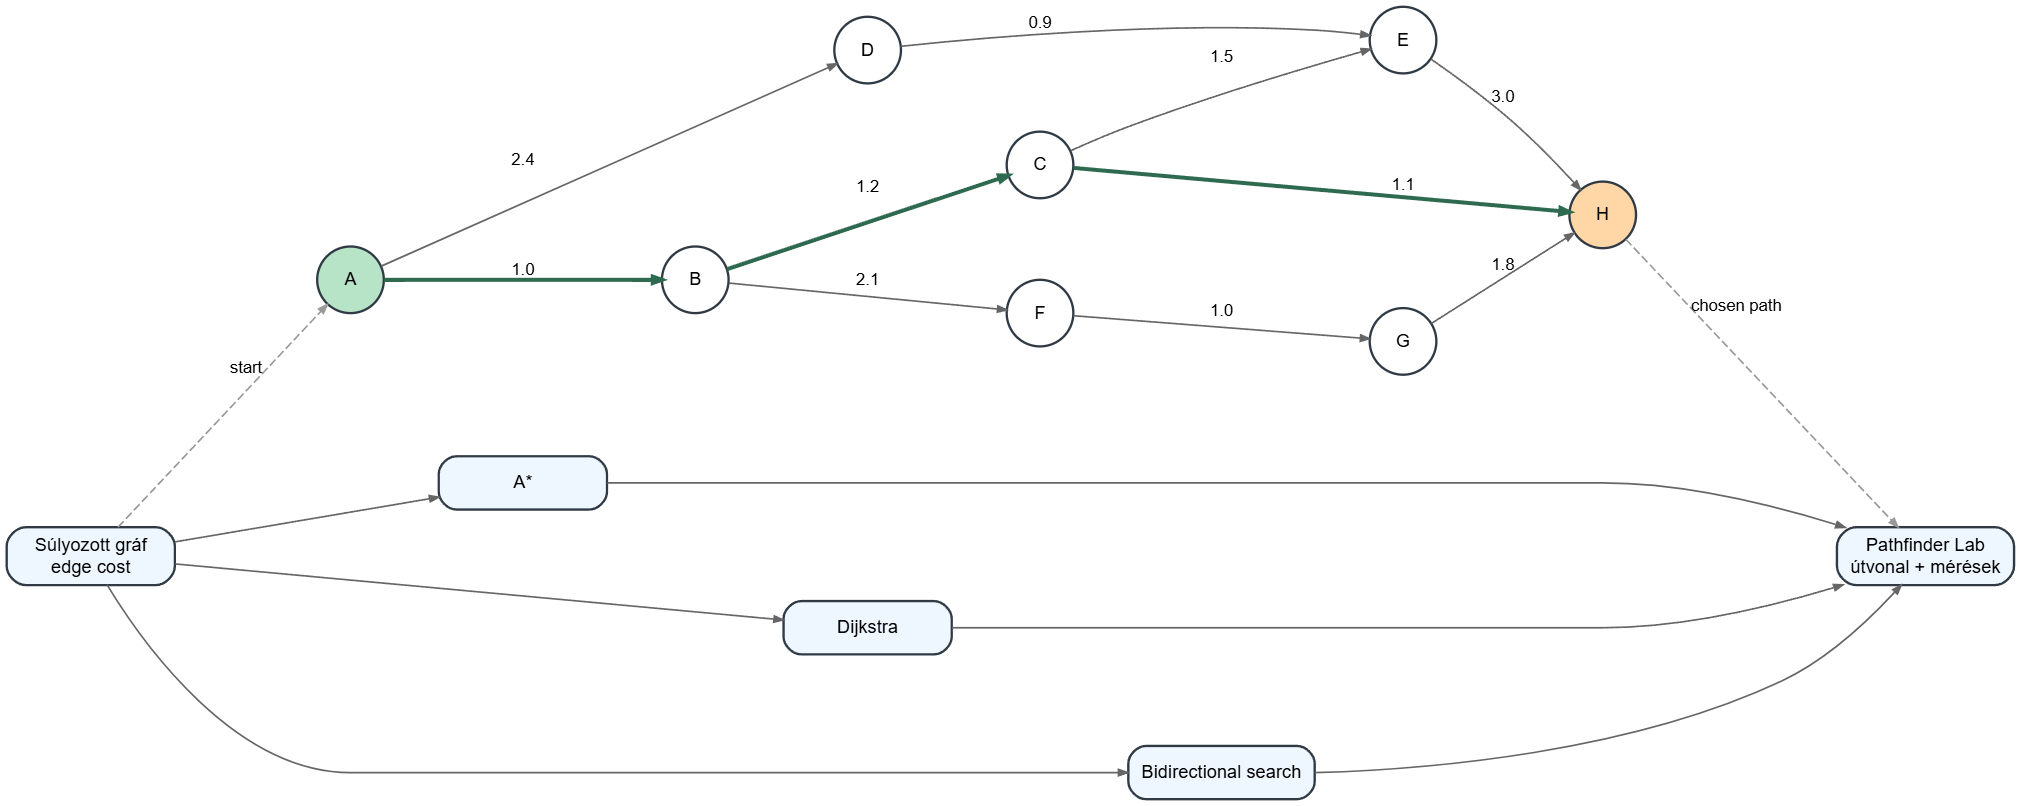
\includegraphics[width=0.92\textwidth]{assets/diagrams/thesis_pathfinding_graphviz.png}
\caption{A Pathfinder Lab algoritmikus értelmezése: ugyanazon súlyozott gráfon több keresési stratégia futtatható, majd az eredmény a replay és mérési rétegen keresztül válik összehasonlíthatóvá.}
\label{fig:pathfinder-graphviz-overview}
\end{figure}

\diagramfigure{A Pathfinder Lab és a frontend komponensstruktúrája - a keresési kérelmek útja a React nézettől a Rust motorig}{path finder and frontend component diagram.pdf}

\subsection{Szélességi keresés (BFS)}

A BFS súlyozatlan módban garantáltan a minimális lépésszámú útvonalat adja. Az implementáció FIFO-sort (\textit{VecDeque}) tart fenn és leáll, amint a célcsomópont először felbukkan a szomszédsági listán. A trace-rögzítés jól mutatja, hogyan terjed ki a keresési határ egyenletesen minden irányban.

\diagramfigure{BFS futtatás a Pathfinder Labban - az egyenletes szélességi terjeszkedés és a minimális ugrásszámú útvonal jól látható a replay állapotban}{pathfinder-bfs-testrun.png}

\subsection{Dijkstra-algoritmus}

A Dijkstra-algoritmus \cite{dijkstra1959} bináris kupacot (\textit{BinaryHeap}) használ. A \textit{QueueState} struktúra lexikografikusan rendez: először az alacsonyabb \textit{cost}, másodlagosan az alacsonyabb csomópont-id szerint, ami garantálja, hogy azonos súlyú utak esetén determinisztikusan mindig ugyanazt az útvonalat kapjuk. Súlyozott módban a rendszer valóban a közvetett, de erős útvonalat preferálja a gyenge közvetlen éllel szemben.

\subsection{Kétirányú keresés}

A kétirányú BFS a forrásból és a célból párhuzamosan terjeszt ki egy-egy keresési frontot, és megáll, amint a két front találkozik. Az implementáció felváltva bővíti a forrás-oldali és a cél-oldali sort. Sűrű vagy nagy gráfokban a meglátogatott csomópontok száma közelítőleg $O(\sqrt{n})$ lehet az egyirányú $O(n)$-hez képest; a tényleges gyorsulás a klaszteres gráfon méréssel ellenőrizhető.

\subsection{A* keresés}

Az A* \cite{hart1968} a Dijkstra-algoritmust terjeszti ki célirányos heurisztikával. Az \textit{AStarState} a \textit{path\_cost} és a \textit{heuristic\_cost} összegével rendez. A heurisztika a \textit{GraphState}-ben előre kiszámított landmark-távolságok táblájából és \textit{cluster\_hops} adatból kombinál admisszibilis alsó becslést, így az A* helyes legrövidebb utat ad. Az egységtesztek igazolják, hogy az A* eredménye egyezik a Dijkstra-eredménnyel minden releváns esetben; csak a keresési sorrend más.

\section{Egzakt A* és heurisztika}

\subsection{Landmark-alapú ALT heurisztika}

Az ALT (A* + Landmarks + Triangle inequality) heurisztika \cite{goldberg2005} a következő elvből indul ki. Ha $L$ egy landmark-csomópont és $d(u, L)$ az $u$ csomópontból $L$-be vezető ismert távolság, akkor:

\begin{equation}
d(u, t) \geq |d(L, t) - d(L, u)| \quad \text{minden } L \text{ landmarkra}
\end{equation}

A rendszer az összes konfigurált landmarkra kiszámolja ezt a korlátot, és a maximumukat adja heurisztikaként. A landmark-távolságok a \textit{GraphState} felépítésekor előre kiszámítódnak minden \textit{ModeKey} kombinációra (SocialUnweighted, SocialWeighted, BattleUnweighted, BattleWeighted) Dijkstra-futtatással, és az összes keresési kérésre újrafelhasználhatók.

\subsection{Landmark-kiválasztás}

A \textit{choose\_landmarks()} a kiindulási landmark-halmazt prioritás alapján állítja össze: előbb hybrid cluster bridge-csomópontok (nagy valószínűséggel sok legrövidebb úton vannak), majd klaszterközéppontok, végül egyéb nagy fokszámú csomópontok. Ez garantálja, hogy a landmarkok a gráf szemantikailag fontos helyein legyenek, ahol a legjobb (legmagasabb) alsó becsléseket adják.

\subsection{Klaszterugrás-alapú becslés és tie-break}

A \textit{cluster\_hops} a forrás és cél klaszter közötti minimális klaszterugrásokon alapul, egy külön Dijkstra-futtatás eredménye a klaszter-szintű gráfon. Admisszibilis korlát, mert bármely útvonalnak legalább annyit kell haladni klasztereken keresztül, mint az inter-klaszter legrövidebb út. A tie-break a klaszterközpont-távolság alapján bont döntetlen azonos becsült összköltség esetén. A képernyőn látható közelség és a gráfbeli költség nem azonos fogalom; ha a rendszer a layoutot valódi heurisztikaként használná, az könnyen inadmisszibilissé tenné a keresést, ezt a megoldás tudatosan kerüli el.

\section{Pathfinder Lab}

A Pathfinder Lab az a réteg, ahol a Rust algoritmusok, a backend-szerződések, a perzisztens játékosprofilok és a böngészőben értelmezhető interakció egyetlen működő demonstrációvá állnak össze. A lab célja nem pusztán az, hogy két játékos között útvonalat megjelenítsen, hanem az, hogy algoritmusonként is láthatóvá tegye, mit jelent ugyanaz a keresési feladat eltérő számítási szemléletekkel megoldani.

A kimenetet a replay panel és a vizuális léptetés teszi értelmezhetővé. A motor minden releváns lépéshez képes rögzíteni az aktív csomópontot, a frontier rövidített állapotát, a meglátogatott csúcsok halmazát és a kiemelt éleket. Így a BFS, Dijkstra, kétirányú keresés és A* nem csak végső útvonal-hosszal hasonlítható össze, hanem a bejárási stratégia szintjén is. A magyarázhatóság nem utólagos vizuális díszítés, hanem a keresőmotor válaszformátumának része.

\diagramfigure{A Pathfinder Lab replay panele - az útvonalösszegző, a léptetési vezérlők és a meglátogatott csomópontok statisztikái}{pathfinder-replay-panel.png}

\diagramfigure{Az overlay vezérlőpanel - szünet, sebesség és vizualizációs beállítások a replay lejátszás közben}{pathfinder_replay_overlay.png}

Az alábbi mérési eredmény különösen szemléletes:

\begin{table}[H]
\centering
\caption{BFS és súlyozott keresés összehasonlítása - ugyanazon játékospár, eltérő közelségi fogalmak}
\begin{tabularx}{\textwidth}{>{\raggedright\arraybackslash}p{3cm} >{\raggedright\arraybackslash}p{3cm} >{\raggedright\arraybackslash}p{2cm} X}
\toprule
\textbf{Algoritmus} & \textbf{Metrika} & \textbf{Eredmény} & \textbf{Értelmezés} \\
\midrule
BFS & Minimális ugrásszám & 3 & Legrövidebb szociális lánc \\
Dijkstra & Min. súlyozott költség & 8 & Legerősebb szövetségesi útvonal \\
A* & Min. súlyozott költség & 8 & Egyezik Dijkstrával \\
Kétirányú & Min. ugrásszám & 3 & Egyezik BFS-sel \\
\bottomrule
\end{tabularx}
\end{table}

A BFS által talált 3-ugrás-os útvonal strukturálisan létezik, de gyenge vagy egyszeri meccsből eredő kapcsolatokon halad át. A Dijkstra súlyozott módban elkerüli ezeket, és helyette egy 8-ugrás-os útvonalat talál, amelyen minden él ismétlődő szövetségesi viszony. A két eredmény nem ellentmond egymásnak: két különböző közelségi fogalmat mér. Súlyozatlan módban a strukturális távolság a kérdés, a Milgram-féle ugrásos közelség értelmében \cite{milgram1967}; súlyozott módban a relációs gerinc kerül felszínre, melyik a legerősebb szövetségesi lánc. Granovetter \cite{granovetter1973} gyenge kapcsolatok elvének analógiájával: a gyenge kapcsolatok (BFS-útvonal) jobb információterjedési csatornák, az erős kapcsolatok (Dijkstra-út) határozzák meg a tényleges közösségi határokat. A BFS=3/Dijkstra=8 divergencia megmutatja, hogy a gráf látszólagos összefüggésének mekkora hányada valódi ismétlődő kapcsolatokból és mekkora alkalmi meccsfelállításokból ered.

\diagramfigure{A* keresés súlyozatlan módban - mindössze 60 csomópontot látogat meg a BFS 5906-ával szemben, mégis azonos 3-ugrás-os eredményt ad; a heurisztika egyenesen a célba irányítja a keresést}{pathfinder-astar-unweighted-testrun.png}

\diagramfigure{A* keresés súlyozott módban - a landmark heurisztika és a klaszter-alapú alsó becslés relációs erősség mentén irányítja a bejárást}{pathfinder-astar-weighted-testrun.png}

\diagramfigure{Az összes algoritmus futtatása súlyozatlan módban - BFS, Dijkstra, kétirányú és A* egységes összehasonlítása azonos játékospáron}{pathfinder-algocomparision-unweighted-test.png}

\diagramfigure{Az összes algoritmus futtatása súlyozott módban - Dijkstra és A* eltér a BFS és kétirányú keresés eredményétől; a heurisztikák csak súlyozott módban aktívak}{pathfinder-algocomparision-weighted-test.png}

\begin{table}[H]
\centering
\caption{A négy algoritmus összehasonlítása a legfontosabb dimenziók mentén}
\begin{tabularx}{\textwidth}{>{\raggedright\arraybackslash}p{3cm} >{\raggedright\arraybackslash}p{2.5cm} >{\raggedright\arraybackslash}X >{\raggedright\arraybackslash}X}
\toprule
\textbf{Algoritmus} & \textbf{Optimális?} & \textbf{Memória} & \textbf{Fő erősség a projektben} \\
\midrule
BFS & Igen (súlyozatlan) & $O(n)$ & Egyszerű baseline, jól magyarázható replay \\
Dijkstra & Igen (súlyozott) & $O(n + m)$ & Referencia-algoritmus, lexikografikus döntetlen-kezelés \\
Kétirányú & Igen (súlyozatlan) & $O(n)$ & Potenciális gyorsulás klaszteres gráfon \\
A* & Igen (heurisztika elfogadható) & $O(n)$ & Célirányos bejárás, egzakt eredmény \\
\bottomrule
\end{tabularx}
\end{table}

\section{Backend orchestráció}

A Rust analitikai parancsfolyam parancsvezérelt háttérfolyamat. A frontend HTTP/JSON kérést küld a Node.js backendnek, a backend a \textit{rustBridge.js} rétegen keresztül indítja vagy újrahasznosítja a Rust CLI folyamatot, és a tényleges parancs stdin csatornán JSON-ként jut el a Rust motorhoz, a válasz stdout-on érkező JSON objektumként kerül vissza. A Node réteg vezérlő és integrációs héj: kezeli a datasetváltást, üríti a régi runtime-állapotot, átadja az aktuális útvonalakat a Rust motornak és a frontend felé csak a fogyasztható választ adja tovább.

\begin{figure}[H]
\centering
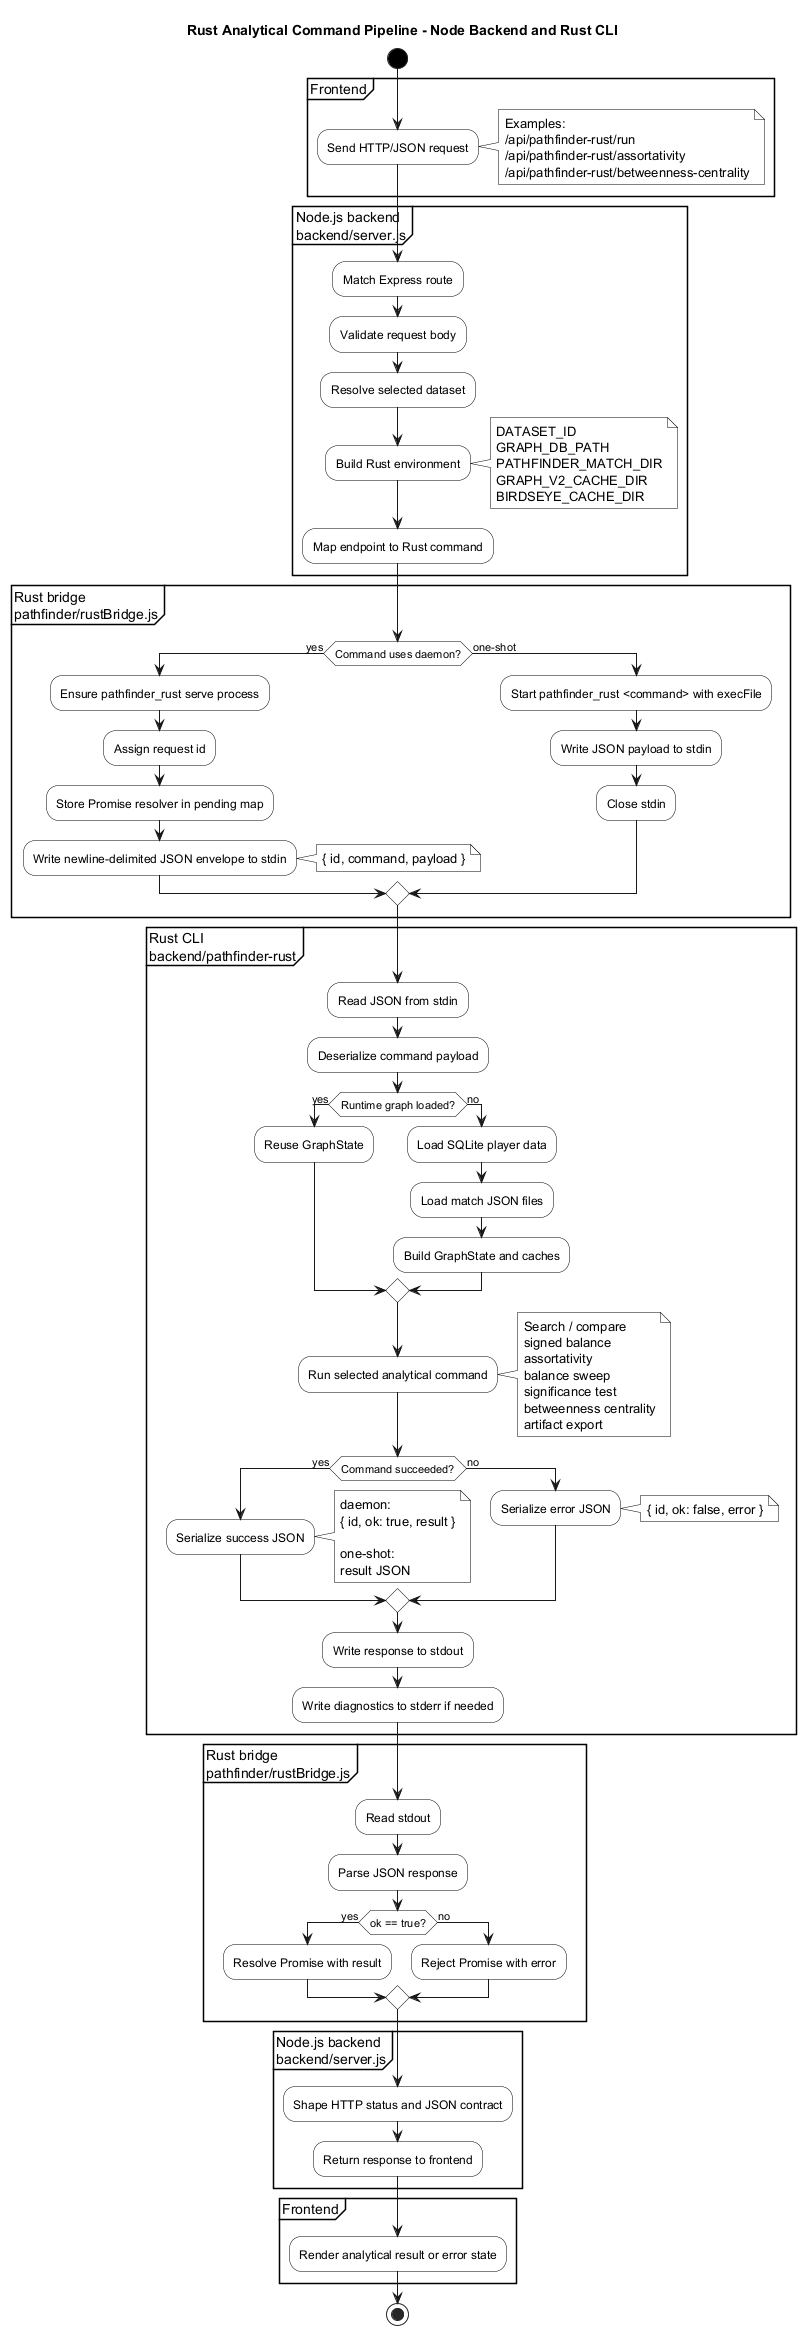
\includegraphics[width=\textwidth,height=0.90\textheight,keepaspectratio]{rust-analytics-cli-pipeline.png}
\caption{A Node.js backend és a Rust CLI közötti parancsvezérelt kommunikáció sémája}
\label{fig:rust-analytics-command-flow}
\end{figure}

A Rust motor \textit{serve} módja stdin/stdout alapú kérés-válasz borítékokkal működik, ami lehetővé teszi, hogy ugyanaz a motor önálló parancssori eszközként és backend mögötti alfolyamatként is használható legyen. A dataset-váltás nem csupán konfigurációs bit-váltás: a motor teljes újraépítést végez, betölti az adott dataset meccs-JSON-jait, klasztereit és játékosprofilját, majd újraszámolja a landmark-távolságokat és a min-cost táblát. A \textit{flexset} esetén ez a teljes 4980 meccset és 5741 csúcsot érinti, és néhány másodpercig tart.

\section{A 3D globális vizualizáció}

A \textit{bird's-eye sphere} a teljes hálózat vizuális áttekintésére szolgál. A legfontosabb tervezési döntés az volt, hogy a böngésző ne valós időben számolja a teljes layoutot: a Rust réteg előre exportál minden fontos artifaktumot, és a frontend csak renderel. Ez determinisztikusabb layoutot, megismételhető demókat és kisebb böngészőterhelést ad, miközben a vizuális réteg jól elválik a számítási rétegtől.

Fontos különbséget tenni a teljes bird's-eye gömb-export és a Graph V2 artifact között. A bird's-eye gömb az összes látható játékost és élkapcsolatot rendereli bele a 3D térbe, míg a Graph V2 csak a minimum szövetségesi támaszú, klasztertagságú csomópontokat tárolja elemzésre alkalmas formában; a két struktúra ezért különböző csúcsszámot mutat ugyanarra a datasetre.

A \textit{flexset} dataset Graph V2 artifaktuma: \textbf{5741} látható csúcs, \textbf{18\,548} látható él, ebből \textbf{13\,572} ally-jellegű (73,17\%) és \textbf{4976} enemy-jellegű (26,83\%), \textbf{1531} klasztercsoport, átlagos klaszterméret \textbf{3,750}, legnagyobb \textbf{20}, generálási idő \textbf{87\,472 ms}. A \textit{soloq} dataset: \textbf{1538} csúcs, \textbf{4111} él, \textbf{2682} ally-jellegű (65,24\%) és \textbf{1429} enemy-jellegű (34,76\%), \textbf{870} klasztercsoport, átlagos klaszterméret \textbf{1,768}, generálási idő \textbf{55\,674 ms}. A két dataset ally/enemy arányának különbsége (flexset: 73/27, soloq: 65/35) strukturálisan értelmes: a Flex Queue csapatonként ötfős játékstílusa természetesen dúsítja az ally-kapcsolatokat, míg a Solo/Duo Queue véletlenszerűbb csapatbeosztása az ellenfél-találkozások arányát növeli.

A Graph V2 vizualizáció asszociatív játékosgráfként értelmezendő, nem barátsági vagy ellenségességi hálóként. A legerősebb minta a core-periphery szerkezet: a központi régióban sok kereszt-klaszter szövetségesi kapcsolatot hordozó csoport jelenik meg, a külső gyűrűben sok kis, gyengén kapcsolt lokális ally-csoport. A \textit{flexset} artifactban 1531 bounded ally-csoport szerepel, ebből 815 bridge-jelölt klaszter és 716 külső, cross-cluster ally hídtalan csoport. A radiális pozíció kulcsjelzés: kisebb orbit-radius erősebb hídjellegű visszatérő ally-kapcsolatokra utal.

\begin{table}[H]
\centering
\caption{A bird's-eye export fő artifaktumai}
\begin{tabularx}{\textwidth}{>{\raggedright\arraybackslash}p{4.2cm}X}
\toprule
\textbf{Fájl} & \textbf{Szerep} \\
\midrule
\textit{manifest.json} & Metaadatok, darabszámok, skálázási és generálási információk \\
\textit{node\_meta.json} & Csomópontszintű leíró metaadatok, frontend-hozzárendelések \\
\textit{node\_positions.f32} & Lebegőpontos koordináták tömbje a gyors rendereléshez \\
\textit{node\_metrics.u32} & Tömörített numerikus csomóponti mutatók \\
\textit{edge\_pairs.u32} & Él-végpontpárok tömbje \\
\textit{edge\_props.u32} & Élhez tartozó kódolt tulajdonságok \\
\bottomrule
\end{tabularx}
\end{table}

A nagy tömegű numerikus adat bináris marad (\textit{.u32} formátum), ami gyorsabb böngészőoldali feldolgozást tesz lehetővé; az emberileg olvasható metaadat külön JSON-rétegben marad. A frontend megjelenít, nem újraszámol.

\begin{figure}[H]
\centering
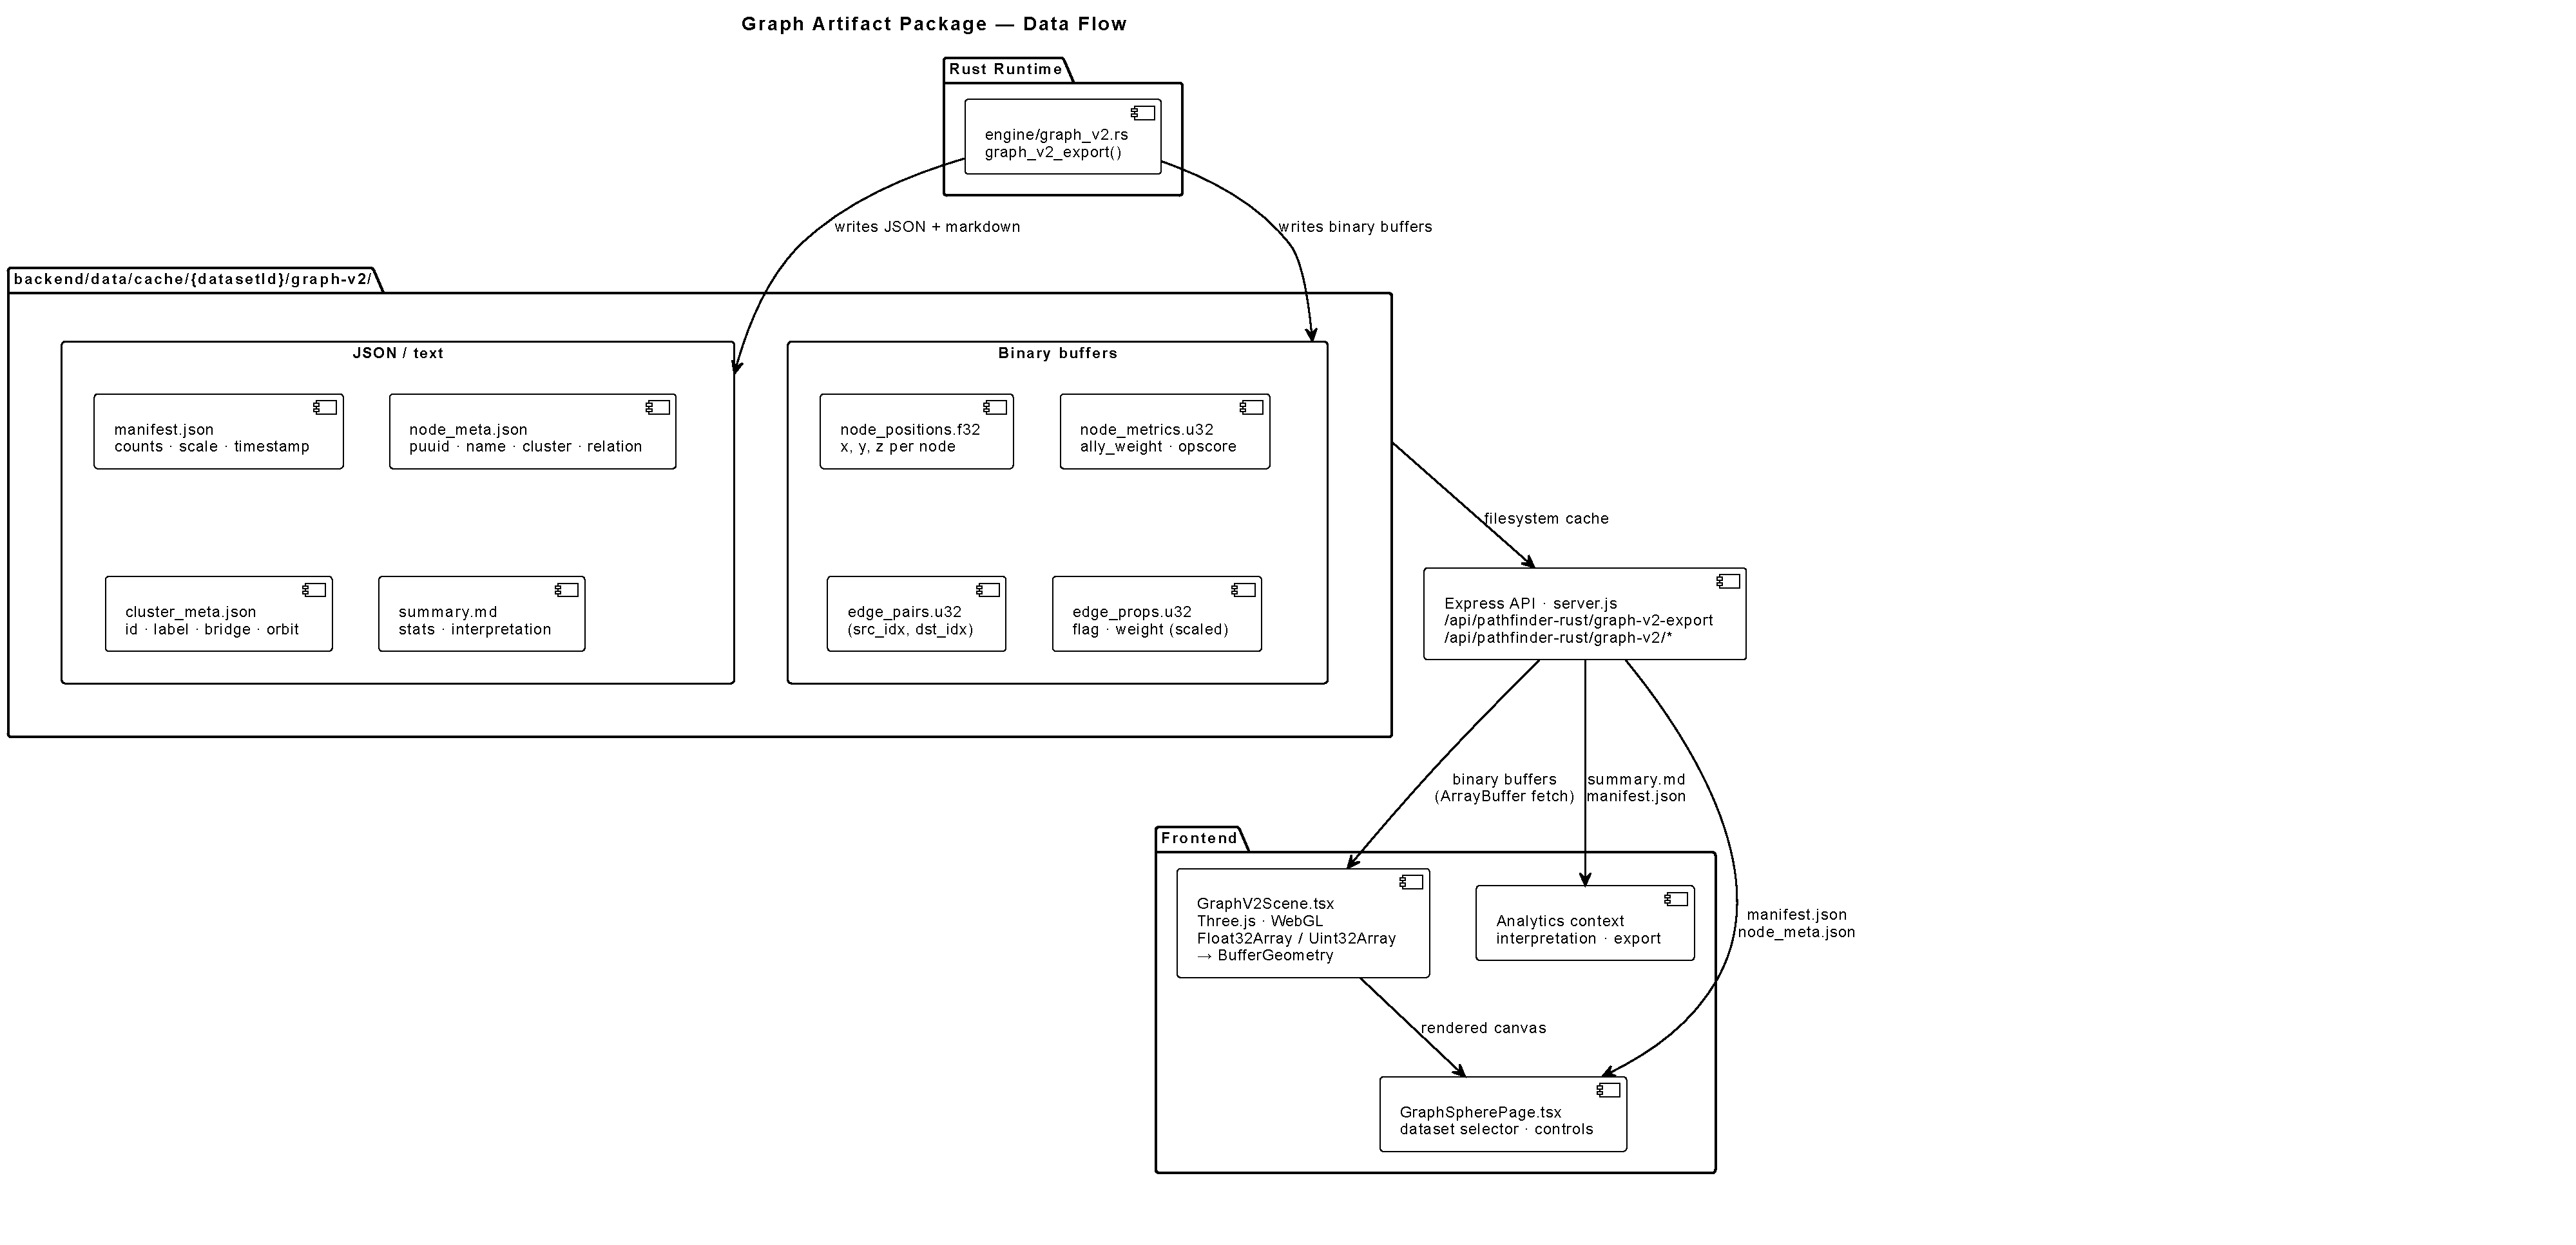
\includegraphics[width=\textwidth,height=0.88\textheight,keepaspectratio]{graph artifact package dataflow.pdf}
\caption{A Graph V2 artifaktumcsomag adatfolyama: a Rust-exportőr bináris és JSON-rétegeket ír, az Express API kiszolgálja, a frontend WebGL-renderelőbe és elemzési kontextusba fogyasztja}
\end{figure}

\begin{figure}[H]
\centering
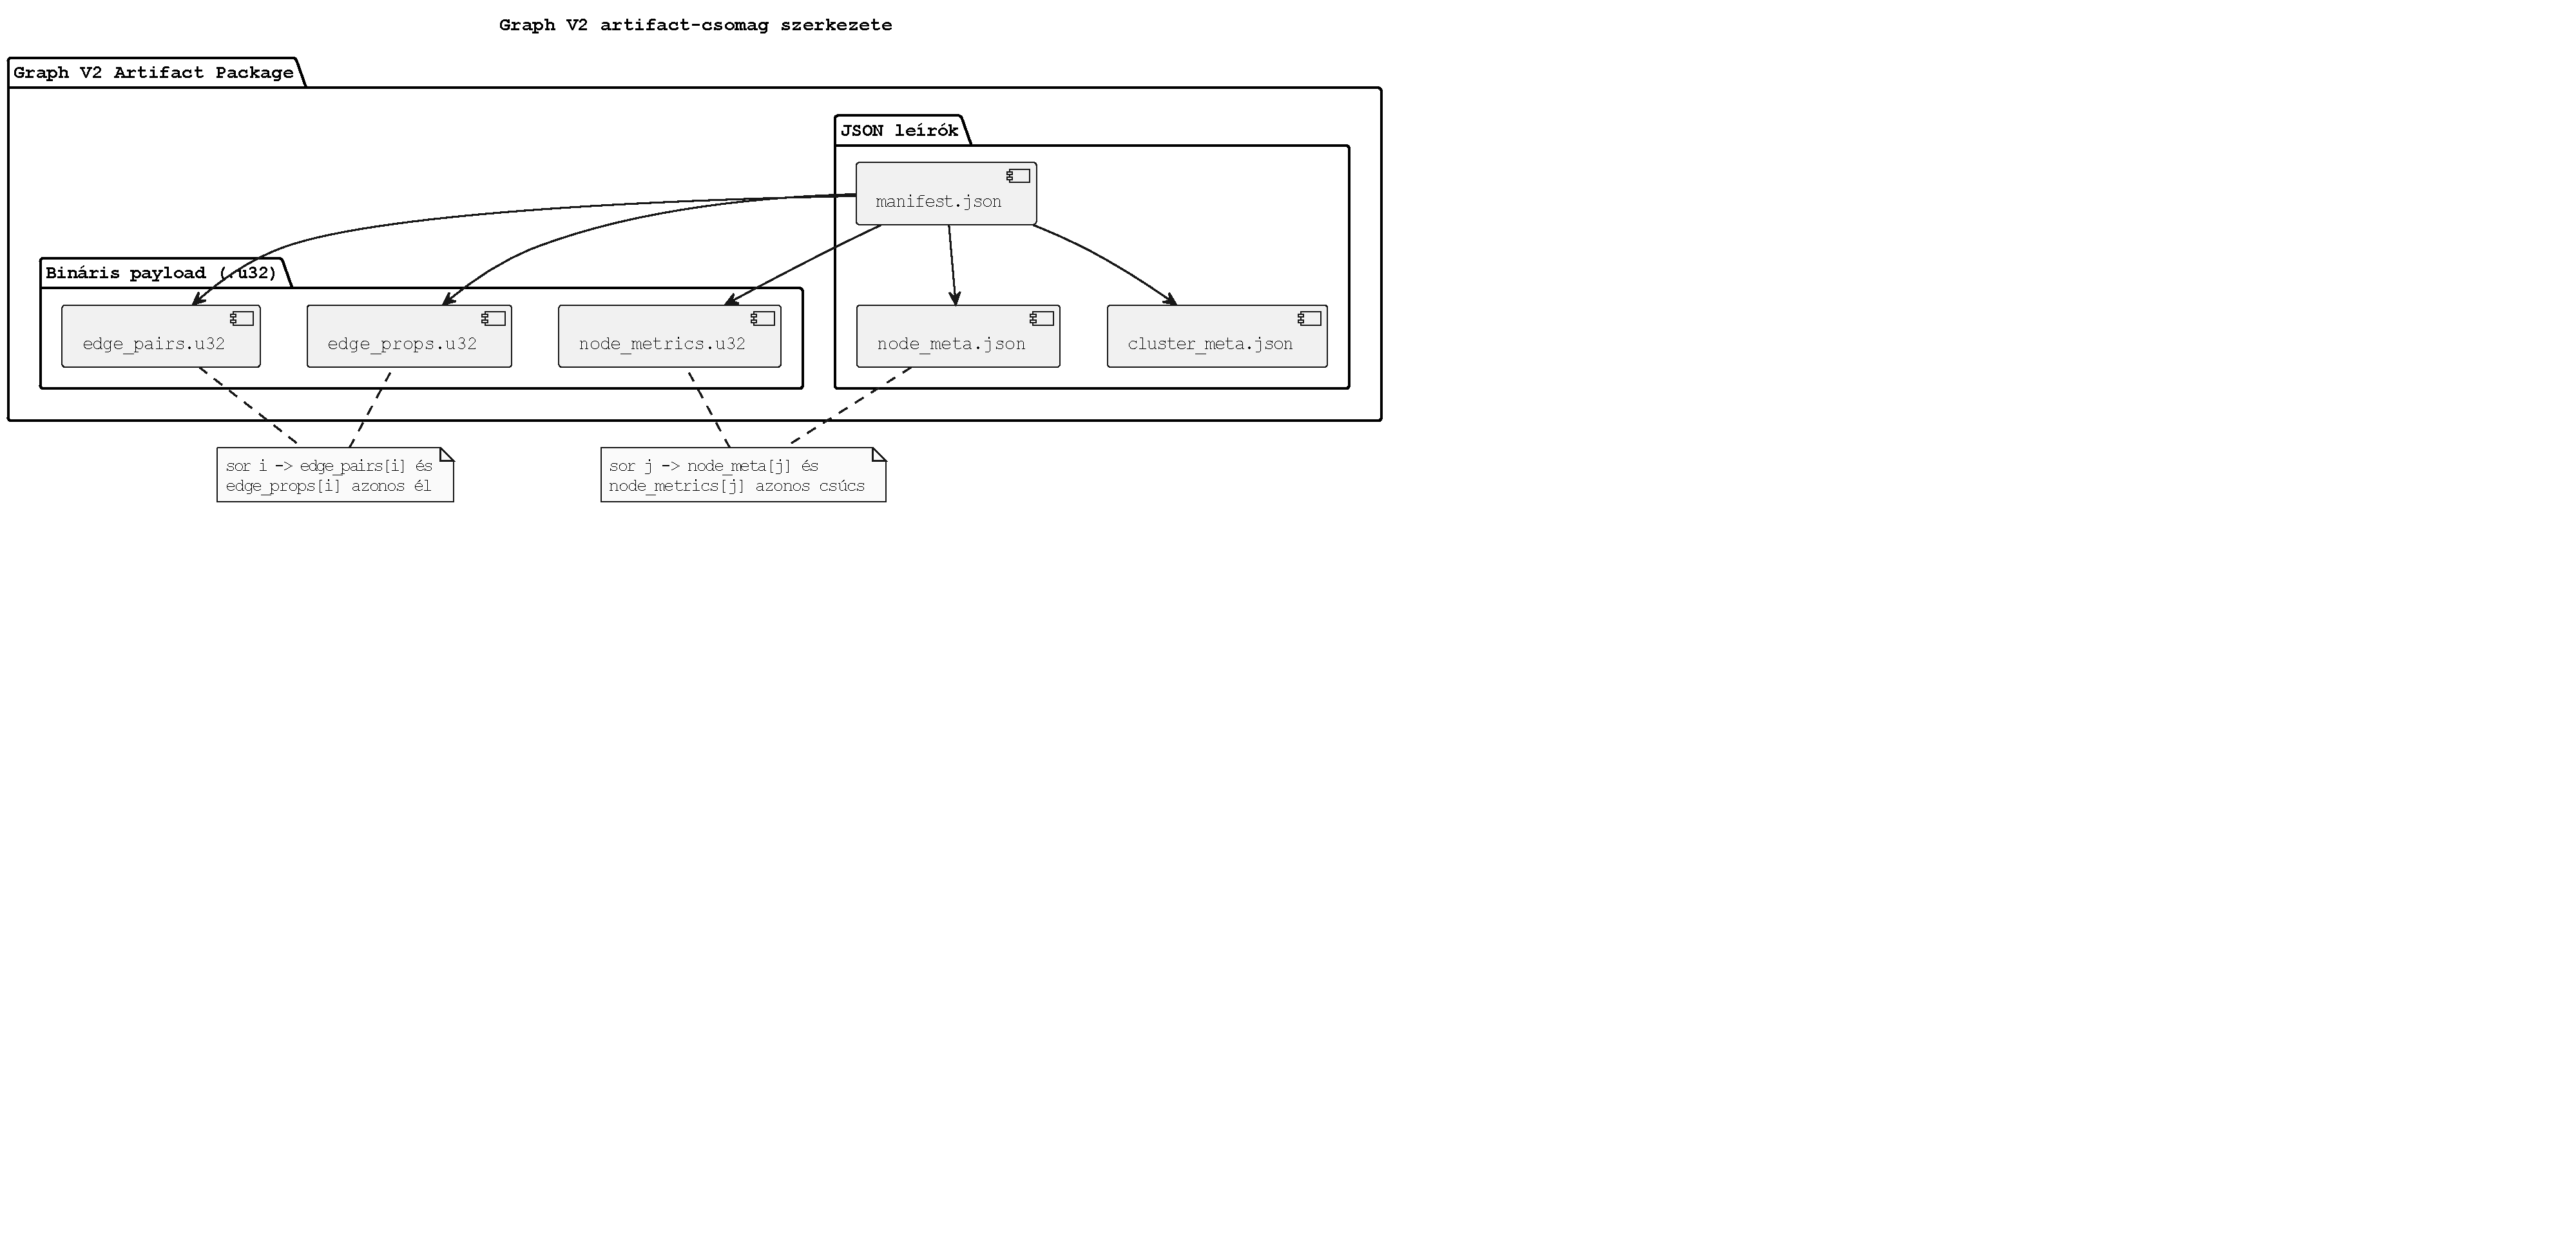
\includegraphics[width=\textwidth,height=0.86\textheight,keepaspectratio]{graph artifact components.pdf}
\caption{A Graph V2 pipeline bináris és JSON artifact-fájljainak szerkezete. A diagram a \texttt{graph-v2-artifact-structure.puml} forrás alapján különíti el a JSON leírókat (\texttt{manifest.json}, \texttt{node\_meta.json}, \texttt{cluster\_meta.json}) és a little-endian \texttt{.u32} bináris payloadokat (\texttt{edge\_pairs.u32}, \texttt{edge\_props.u32}, \texttt{node\_metrics.u32}). A \texttt{manifest.json} tartalmazza a csúcs-, él- és klaszterszámokat, míg a párhuzamos indexelés biztosítja, hogy az azonos sorszámú metadata- és metric-sor ugyanarra a csúcsra, illetve az azonos sorszámú edge-pair és edge-prop rekord ugyanarra az élre vonatkozzon.}
\end{figure}

\begin{figure}[H]
\centering
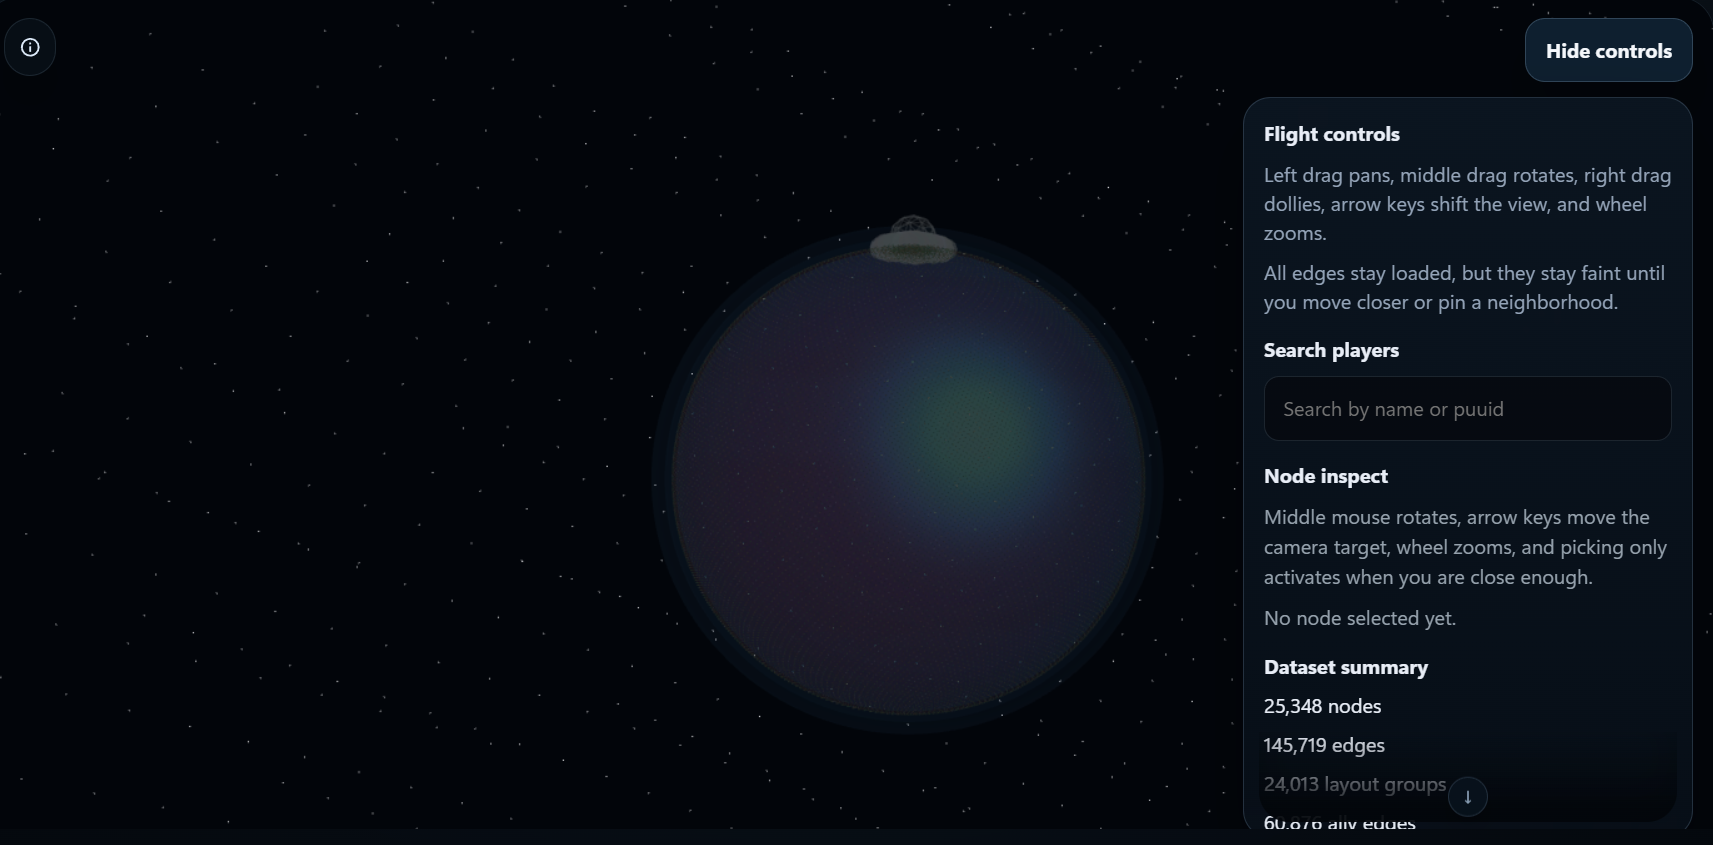
\includegraphics[width=0.98\textwidth,height=0.72\textheight,keepaspectratio]{birds-eye-current-state.png}
\caption{A teljes hálózat 3D madártávlati nézete az előre generált Rust-artifaktumokra építve}
\end{figure}

\begin{figure}[H]
\centering
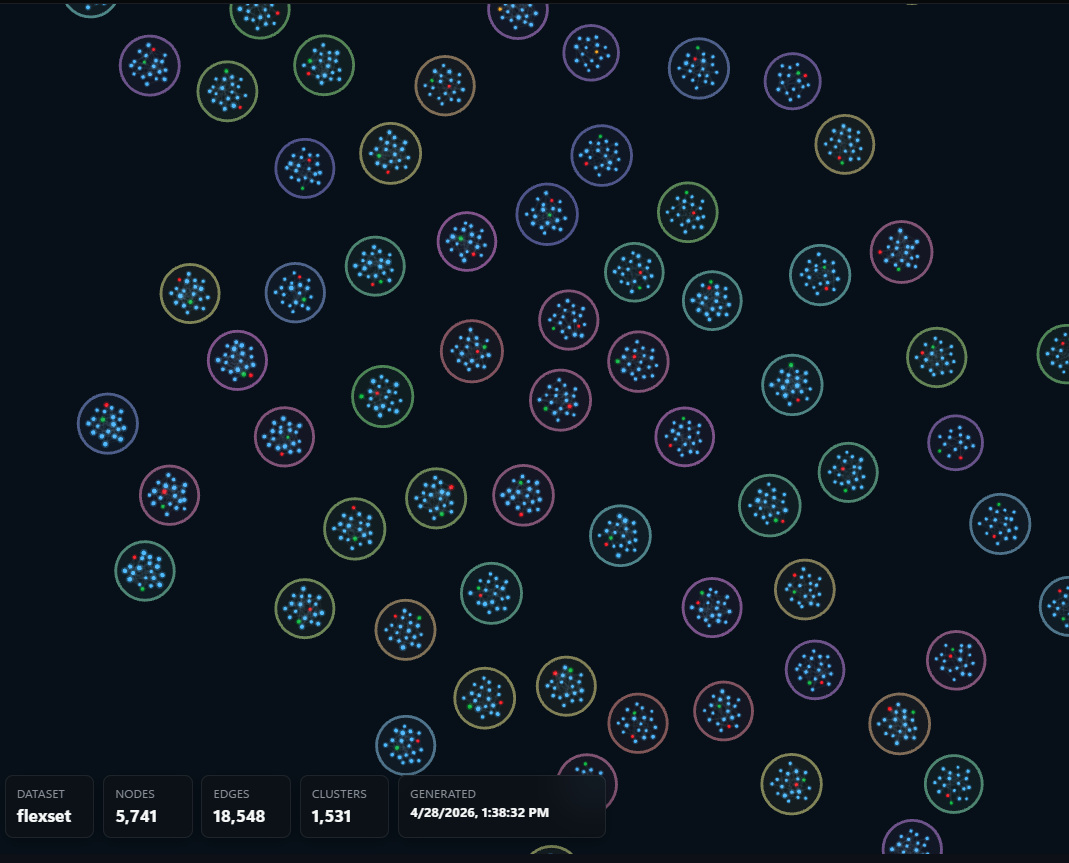
\includegraphics[width=0.98\textwidth,height=0.72\textheight,keepaspectratio]{flexset_associative_graph_clusters.png}
\caption{Sűrűbb klaszterfoltok és a térbeli elkülönítés a globális nézetben}
\end{figure}

\section{A strukturális egyensúly mint módszertani határeset}

A repositoryban megvalósított \textit{signed\_balance.rs} modul determinisztikusan előállít egy előjeles egyszerű gráfot, teljesen összekapcsolt triádokat enumerál, majd a Heider--Cartwright--Harary-féle szabály szerint osztályozza őket. A visszaminősítés oka nem technikai, hanem szemantikai: az \textit{allyWeight} dominanciája pozitív élként kezelhető, mert a Flex Queue-ban a visszatérő csapattársi viszony részben szándékolt együttjátszást is tükrözhet, de az \textit{enemyWeight} dominanciája technikailag negatív élként jelölhető, ez nem azonos ellenségességgel, rivalizálással vagy elutasítással. Az ismételt szembekerülés hasonló MMR-sávból, azonos napszakból, a Master$+$ Flex Queue kis aktív játékospoolából, matchmaking-ismétlésből vagy az adatgyűjtési stratégia torzításából is adódhat.

Ezért az \textit{enemyWeight} negatív signed-network élként való kezelése túl erős állítás lenne a dolgozat fő empirikus narratívájához. A döntetlen-kezelés, a minimum support és a triádenumerálás auditálható és újrafuttatható; a kapott arányok azonban inkább a választott projekció viselkedését mutatják, nem pedig bizonyított társas egyensúlyt. A modul a repositoryban kísérleti opcióként megmaradhat, mert hasznos módszertani tanulságot ad: egy formálisan elegáns gráfelméleti módszer hogyan válhat interpretációs szempontból gyengévé, ha az él szemantikája nem felel meg az elmélet előfeltevéseinek. A signed-balance oldal és a kombinált futtató kikerül a fő navigációs útvonalból; a dolgozat fő pillérei az asszociatív gráfértelmezés, az asszortativitási eredmények és a Brandes-betweenness centralitás.

% Ez a fejezet összevonásra került a 12-es fejezettel (A Rust futtatókörnyezet, útvonalkeresés és vizualizáció).

\chapter{A 3D bird's-eye sphere és globális hálózati vizualizáció}

\section{A frontend szerepe}

A frontend jelenleg már nem egyetlen gráfnézet, hanem több, világosan elkülönített felületből álló mini-rendszer. Ez fontos minőségi ugrás a korábbi állapothoz képest, mert a projekt ekkor vált valóban bemutatható és narratívába rendezhető alkalmazássá.

A fő felületek:

\begin{itemize}
    \item \textbf{Match Analysis}: adatgyűjtési és mérkőzésellenőrző nézet,
    \item \textbf{Pathfinder Lab}: útvonalkeresési és algoritmus-összehasonlító nézet,
    \item \textbf{Full 3D Graph Sphere}: teljes hálózati madártávlat,
    \item \textbf{Assortativity}: teljesítmény-hasonlóságot vizsgáló analitikai oldal,
    \item \textbf{Betweenness Centrality}: Brandes-központisági és bridge/broker elemző oldal.
\end{itemize}

\section{Miért nem egyetlen képernyő?}

A felület több oldalra bontása nem esztétikai döntés volt, hanem használhatósági és védhetőségi kérdés. Egy szakdolgozati demo során sokkal könnyebb végigvezetni a nézőt azon az úton, hogy:

\begin{enumerate}
    \item adatot gyűjtünk vagy ellenőrzünk,
    \item gráfot és klasztereket generálunk,
    \item útvonalakat keresünk,
    \item globális struktúrát nézünk,
    \item kutatási jellegű elemzést futtatunk.
\end{enumerate}

Ha minden ugyanarra a képernyőre kerülne, a projekt inkább eszköztárnak, mintsem koherens rendszernek hatna.

\section{A 3D globális nézet}

A \emph{bird's-eye sphere} oldal a teljes hálózat vizuális áttekintésére szolgál. A legfontosabb tervezési döntés itt az volt, hogy a böngésző ne valós időben számolja a teljes layoutot, hanem a Rust réteg előre exportáljon minden fontos artifaktumot, és a frontend csak rendereljen.

Ennek több előnye van:

\begin{itemize}
    \item a layout determinisztikusabb,
    \item a demók megismételhetők,
    \item a böngésző terhelése kisebb,
    \item a vizuális réteg jobban elválik a számítási rétegtől.
\end{itemize}

\section{A bird's-eye manifest technikai tartalma}

Fontos különbséget tenni a teljes bird's-eye gömb-export és a Graph V2 artifact között. A bird's-eye gömb az összes látható játékost és élkapcsolatot rendereli bele a 3D térbe, míg a Graph V2 csak a minimum szövetségesi támaszú, klasztertagságú csomópontokat tárolja elemzésre alkalmas formában. A két struktúra ezért különböző csúcsszámot mutat ugyanarra a datasetre.

A \texttt{flexset} dataset esetében a Graph V2 artifact összefoglalója az alábbi adatokat rögzíti:

\begin{itemize}
    \item \textbf{5741} látható csúcs (klasztertagok és hozzájuk kapcsolódó csúcsok),
    \item \textbf{18\,548} látható él,
    \item \textbf{13\,572} ally-jellegű él (73.17\%),
    \item \textbf{4976} enemy-jellegű él (26.83\%),
    \item \textbf{1531} klasztercsoport,
    \item átlagos klaszterméret \textbf{3.750}, legnagyobb \textbf{20},
    \item generálási idő: \textbf{87\,472 ms}.
\end{itemize}

A \texttt{soloq} dataset Graph V2 artifaktuma:

\begin{itemize}
    \item \textbf{1538} látható csúcs,
    \item \textbf{4111} látható él,
    \item \textbf{2682} ally-jellegű él (65.24\%),
    \item \textbf{1429} enemy-jellegű él (34.76\%),
    \item \textbf{870} klasztercsoport,
    \item átlagos klaszterméret \textbf{1.768}, legnagyobb \textbf{20},
    \item generálási idő: \textbf{55\,674 ms}.
\end{itemize}

A két dataset ally/enemy arányának különbsége (flexset: 73/27, soloq: 65/35) szintén strukturálisan értelmes. A Flex Queue-ban a csapatonként öt fő játékstílus természetes módon dúsítja az ally-kapcsolatokat, míg a Solo/Duo Queue véletlenszerűbb csapatbeosztása az ellenfél-találkozások arányát növeli. Ez az arány önmagában is módszertani érv amellett, hogy a \texttt{flexset} erősebb asszociatív játékosgráfot hoz létre, de nem bizonyítja, hogy az enemy-élek negatív társas kötésekként értelmezhetők.

\section{A \texttt{flexset} mint asszociatív core-periphery játékosgráf}

A Graph V2 vizualizációt ebben a dolgozatban nem közvetlen barátsági vagy ellenségességi hálóként, hanem asszociatív játékosgráfként értelmezem. A csúcsok játékosokat, az élek pedig ismétlődő meccsbeli együtt- vagy szembekerülési bizonyítékot jelölnek. A legerősebb minta nem az előjeles egyensúly, hanem a core-periphery szerkezet: a központi régióban sok kereszt-klaszter szövetségesi kapcsolatot hordozó csoport jelenik meg, míg a külső gyűrűben sok kis, gyengén kapcsolt vagy teljesen híd nélküli lokális ally-csoport található.

A \texttt{flexset} artifactban \textbf{1531} bounded ally-csoport szerepel, ezek közül \textbf{815} bridge-jelölt klaszter, míg \textbf{716} külső pályára helyezett csoport nem rendelkezik cross-cluster ally híddal. A legfontosabb vizuális jel nem az, hogy egy klaszter balra vagy jobbra esik-e a képen, hanem a radiális pozíció: a kisebb orbit-radius erősebb hídjellegű, visszatérő ally-kapcsolatokra utal, a külső gyűrű pedig gyengén kapcsolt lokális szigeteket jelöl.

Ez az értelmezés módszertanilag erősebb, mint a signed-balance olvasat, mert nem igényli, hogy az ellenfélként való ismételt találkozást negatív társas kötésnek tekintsük. Elég hozzá az óvatosabb állítás: a Flex Queue match history ismétlődő asszociációs mintázatokat termel, amelyekben lokális ally-csoportok és hídgazdag központi régiók különülnek el.

A teljes rendszer bird's-eye gömb-exportja a backend által előre generált bináris és JSON artifaktumokat fogyaszt, és nem valós idejű számítást végez a böngészőben. Ez a tervezési döntés biztosítja, hogy a nagy gráfok megjelenítése is determinisztikus és reprodukálható maradjon.

A \texttt{server.js} és a bird's-eye exportútvonalak alapján a 3D nézet mögött több, külön felelősségű artifaktum áll. A frontend nem egyetlen nagy JSON-fájlt tölt be, hanem manifesztet és bináris tömböket fogyaszt.

\begin{table}[H]
\centering
\caption{A bird's-eye export fő artifaktumai}
\begin{tabularx}{\textwidth}{>{\raggedright\arraybackslash}p{4.2cm}X}
\toprule
\textbf{Fájl} & \textbf{Szerep} \\
\midrule
\texttt{manifest.json} & Metaadatok, darabszámok, skálázási és generálási információk \\
\texttt{node\_meta.json} & Csomópontszintű leíró metaadatok, frontend-hozzárendelések \\
\texttt{node\_positions.f32} & Lebegőpontos koordináták tömbje a gyors rendereléshez \\
\texttt{node\_metrics.u32} & Tömörített numerikus csomóponti mutatók \\
\texttt{edge\_pairs.u32} & Él-végpontpárok tömbje \\
\texttt{edge\_props.u32} & Élhez tartozó kódolt tulajdonságok \\
\bottomrule
\end{tabularx}
\end{table}

Ez a bontás rendszerszinten jól indokolható. A nagy tömegű numerikus adat bináris marad, ami gyorsabb böngészőoldali feldolgozást tesz lehetővé, miközben az emberileg olvasható metaadat külön JSON-rétegben marad. A frontend tehát megjelenít, nem pedig újraszámol.

\begin{figure}[H]
\centering
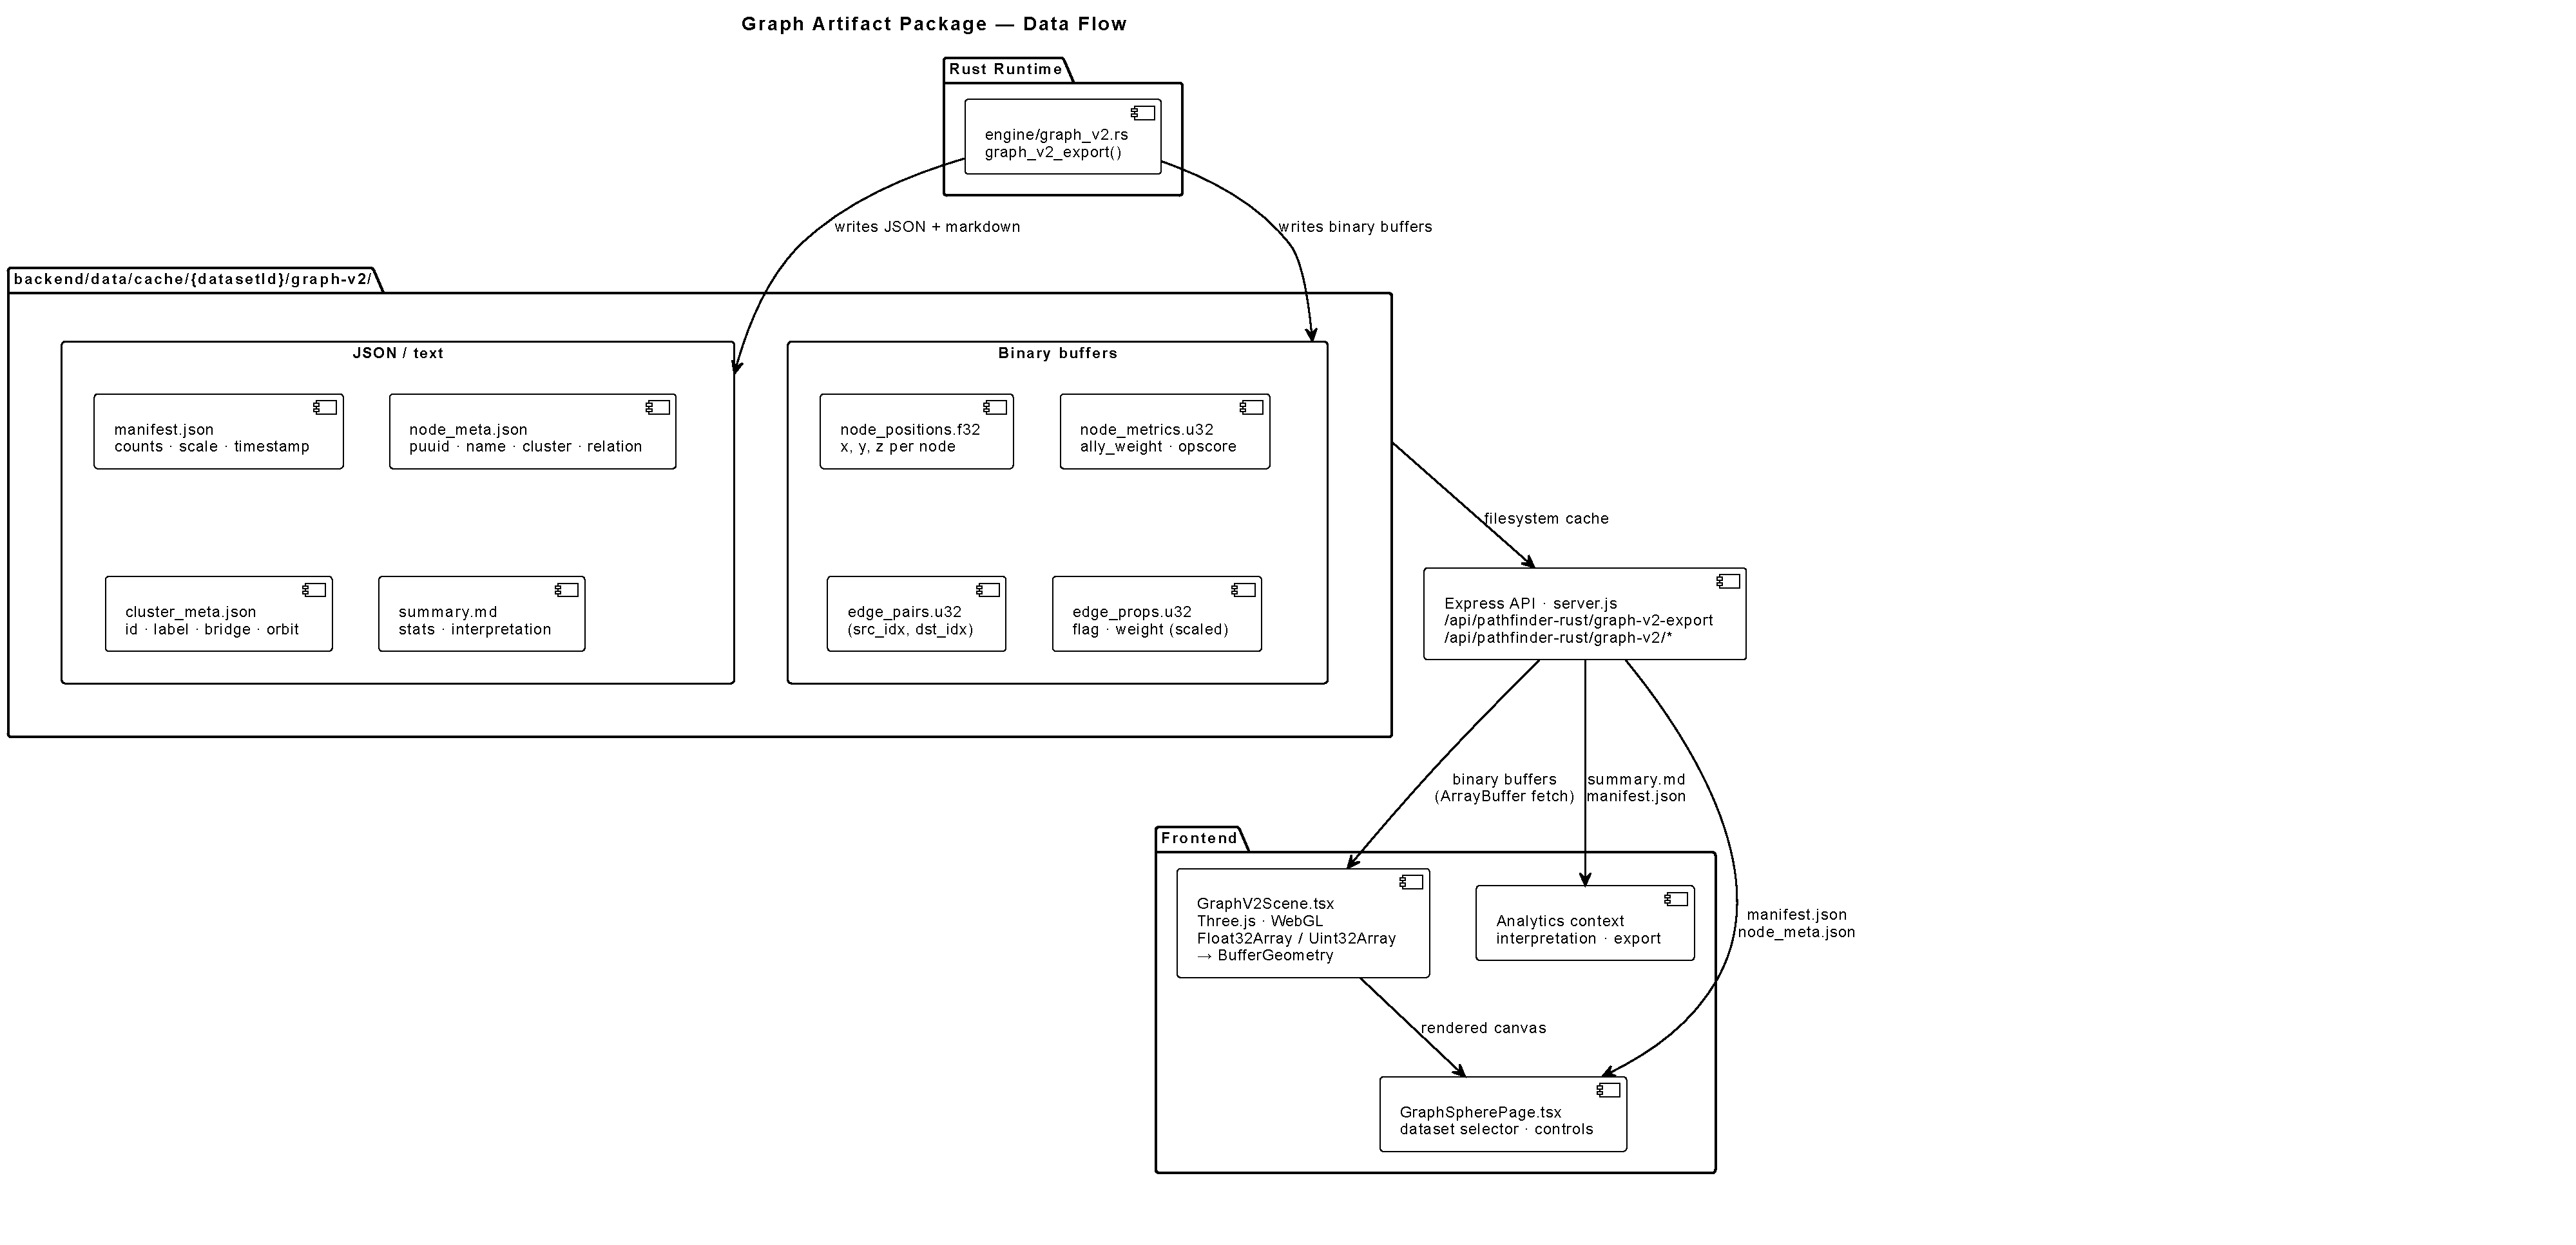
\includegraphics[width=0.95\textwidth,keepaspectratio]{graph artifact package dataflow.pdf}
\caption{A Graph V2 artifaktumcsomag adatfolyama: a Rust-exportőr bináris és JSON-rétegeket ír, az Express API kiszolgálja, a frontend WebGL-renderelőbe és elemzési kontextusba fogyasztja}
\end{figure}

\begin{figure}[H]
\centering
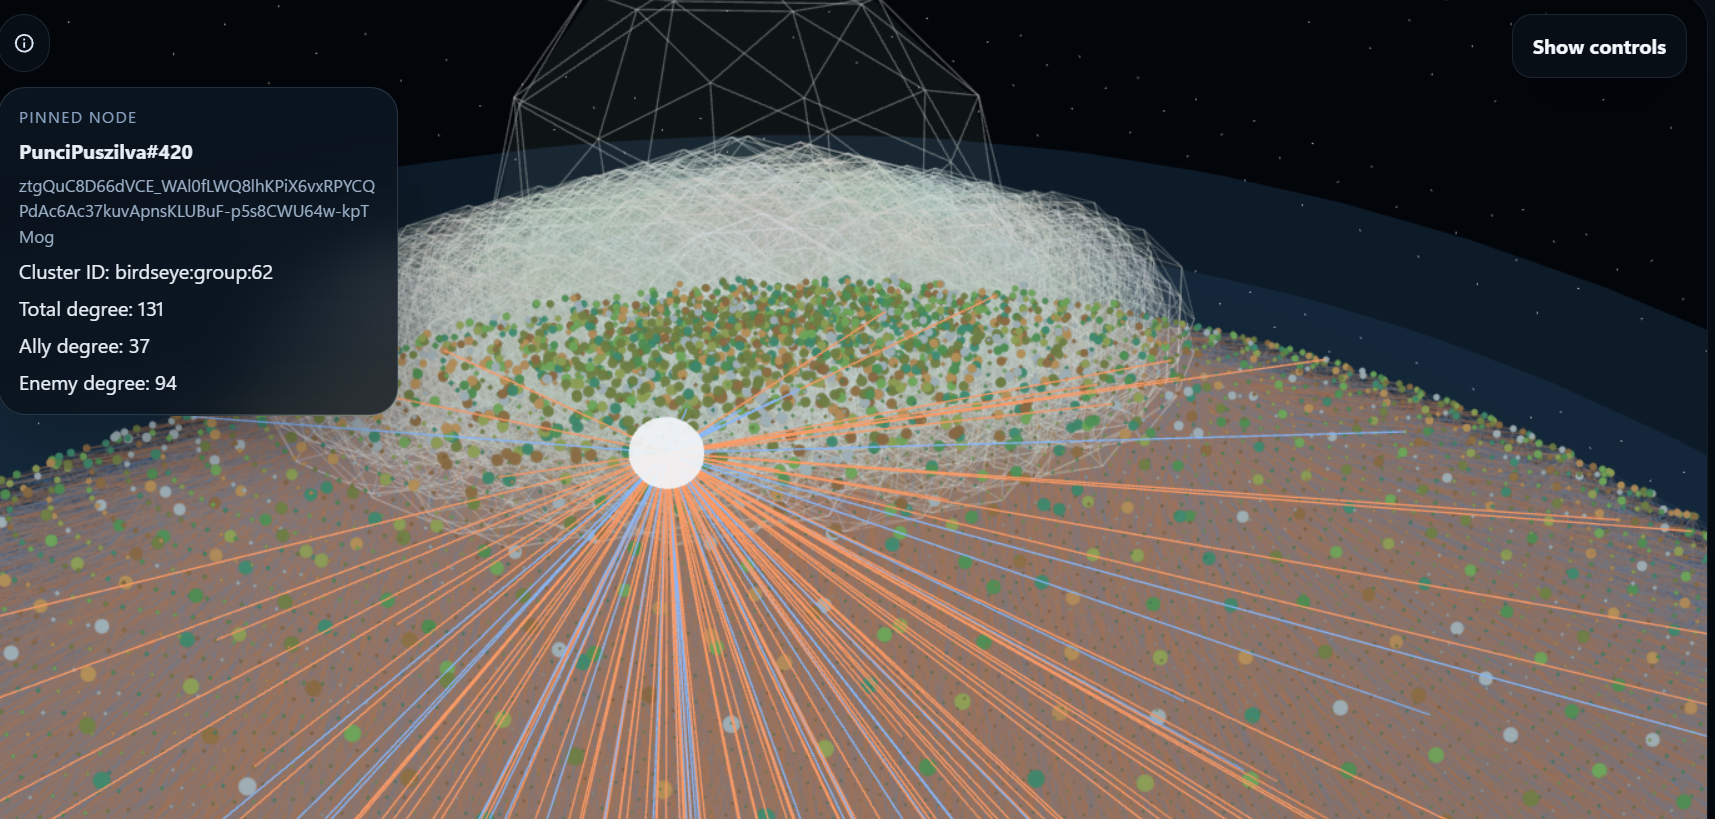
\includegraphics[width=0.98\textwidth,height=0.72\textheight,keepaspectratio]{birds-eye-cluster-view.png}
\caption{A teljes hálózat 3D madártávlati nézete az előre generált Rust-artifaktumokra építve}
\end{figure}

\begin{figure}[H]
\centering
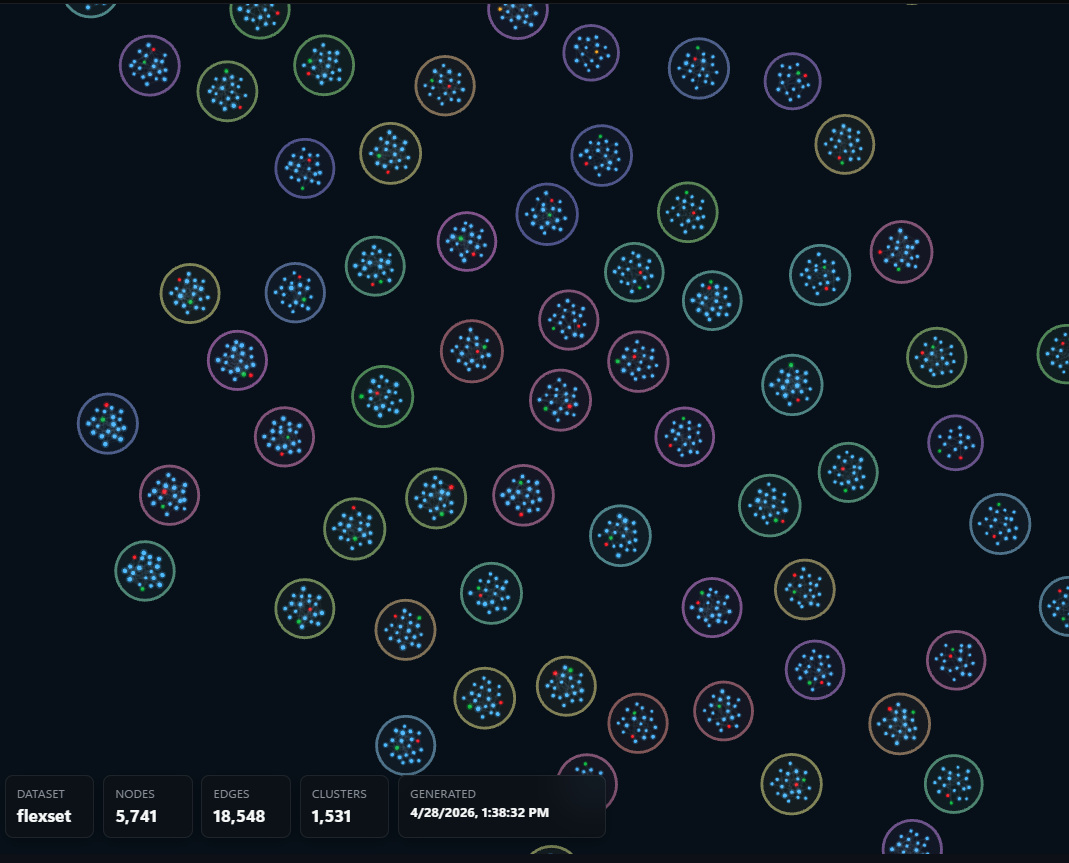
\includegraphics[width=0.98\textwidth,height=0.72\textheight,keepaspectratio]{flexset_associative_graph_clusters.png}
\caption{Sűrűbb klaszterfoltok és a térbeli elkülönítés a globális nézetben}
\end{figure}

\section{Pathfinder Lab}

A Pathfinder Lab az a felület, ahol a gráf nem elsősorban látványelemként, hanem algoritmikus térként jelenik meg. A felület támogatja:

\begin{itemize}
    \item forrás- és céljátékos kiválasztását,
    \item több algoritmus összehasonlítását,
    \item visszajátszási és léptetési funkciókat,
    \item súlyozott és nem súlyozott módot,
    \item többféle útvonalmód közötti váltást.
\end{itemize}

\section{Assortativity és központisági oldalak}

A kutatás-orientált frontend oldalak közös tulajdonsága, hogy nem elégednek meg egyetlen backend-válasz megjelenítésével. Az asszortativitási és központisági nézetek igyekeznek:

\begin{itemize}
    \item magyarázni a kontrollok jelentését,
    \item megmutatni a pipeline-összefüggéseket,
    \item elkerülni a túl gyors, túl erős társadalmi következtetéseket.
\end{itemize}

Ez különösen fontos, mert az ilyen típusú analitika könnyen félreértelmezhető. A felület ezért szándékosan tartalmaz interpretációs szövegeket és magyarázó elemeket is. A signed-balance oldal a jelenlegi dolgozati bemutatási útvonalból kikerült: a hozzá tartozó backend/Rust kód megmaradhat kísérleti opcióként, de a fő navigáció és a bemutatási útvonal már az asszortativitásra, a core-periphery gráfolvasatra és a Brandes-központiságra épül.

\section{Betweenness Centrality oldal}

A \texttt{BetweennessCentralityPage} a projekt egyik legkomplexebb analitikai nézetje. A felület nem pusztán indítja a Brandes-algoritmust, hanem eredményinterpretációs panelekkel, timing-összehasonlítással és döntési dokumentációval egészíti ki az analitikai kimenetet.

A oldal négy fő részből áll:

\begin{itemize}
    \item \textbf{Konfigurációs fejléc}: gráfmód (\texttt{battle-path} / \texttt{social-path}), él-súlyozás, minimum edge support és top-N korlát megadása; négy előre definiált preset (Strong 20, Medium 10, Wide 5, Full 1) gyors paraméterváltáshoz;
    \item \textbf{Projekcióolvasat}: a felület automatikusan értelmezi a megtartott él arányát - ha az arány 1\% alá esik, ``erős kötésű broker elemzés''; 10\% felett ``teljes gráf közelítő elemzés'';
    \item \textbf{Párhuzamossági összehasonlító}: ha a serial baseline futás engedélyezett, a felület megmutatja a serial és parallel futásidőt, a sebességarány-értékelést és a serial--parallel maximális abszolút eltérést (nulla kell legyen, ha a párhuzamosítás determinisztikus);
    \item \textbf{Broker-rangsor}: az első 6 csúcs kártyás nézete (rank, label, klasztercsoport, degree, strength, raw és normalizált BC), majd teljes táblázat.
\end{itemize}

A ``Dokumentált döntések'' panel (algorithm, parallelization, edge support rule, edge cost rule, normalization rule, graph scope) közvetlenül a Rust motor válaszából érkezik: a frontend nem rekonstruálja, hanem visszatükrözi az analitika által rögzített módszertani döntéseket. Ez azt jelenti, hogy a felületen megjelenő szöveges leírások mindig konzisztensek a tényleges futtatással.

Ez a nézet kulcsszerepet játszik a szakdolgozati bemutathatóság szempontjából: nem feketedoboz-eredményt ad vissza, hanem a futás körülményeivel, korlátaival és időbeli teljesítményével együtt prezentálja az eredményt.

\section{Player Detail oldal}

A \texttt{PlayerDetailPage} egy játékos-centrikus nézet, amely a kollektív analitikáktól eltérően egyetlen játékos profiljára fókuszál. Az oldal URL-paraméterrel (\texttt{?puuid=...}) adresszálható, így a Pathfinder Lab más nézeteiből közvetlenül lehet linkelni egy-egy csomópontra.

A nézet két fő részből áll: a játékoskereső mezőből (\texttt{PlayerLookupField}) és a \texttt{PlayerPerformanceCard} komponensből. Ez utóbbi összesíti az adott játékos pontszámait (opscore, feedscore), meccsadatait, szerepkör-eloszlását és klasztertagságát egy lapozás nélküli, pásztázható kártyanézetben.

Az oldal létjogosultsága a rendszerben az, hogy az aggregált elemzések (betweenness centralitás, asszortativitás, útvonalkeresési eredmények) sokszor néhány konkrét csomópontra irányítják a figyelmet. A Player Detail oldal lehetővé teszi, hogy ezek a csomópontok azonnal kontextusban is megvizsgálhatók legyenek, anélkül hogy az elemzőnek a nyers adatbázishoz kellene visszanyúlni.

\section{A Graph V2 artifaktum-pipeline részletei}
\label{sec:graph_v2_artifact}

A Graph V2 pipeline nem egyetlen monolitikus JSON-fájlt hoz létre, hanem egy gondosan megtervezett, kétféle formátumú (bináris és JSON) artifaktum-csomagot, amelyből a frontend oldalak és az analitikai motorok is hatékonyan tudnak táplálkozni.

\subsection{Az artifact-csomag összetétele}

A Graph V2 pipeline a \texttt{backend/data/cache/\{datasetId\}/graph-v2/} könyvtárba generálja a következő fájlokat:

\begin{itemize}
    \item \textbf{manifest.json}: metaadat és méretinformáció - meccszám, csúcsszám, élszám, generálási időbélyeg, verzió;
    \item \textbf{node\_meta.json}: csomópont-azonosítók és metaadatok - puuid, label, klaszterazonosító, pozíció (x, y), hídjelölő státusz;
    \item \textbf{node\_metrics.u32}: bináris, packed uint32 formátum - minden csomóponthoz sorrendben tárolja az opscore és feedscore értékeket egész skálán;
    \item \textbf{edge\_pairs.u32}: bináris élpárok - minden él két csomópont-indexeként tárolva;
    \item \textbf{edge\_props.u32}: bináris éltulajdonságok - allyWeight, enemyWeight, totalMatches minden élhez;
    \item \textbf{cluster\_meta.json}: klaszterszintű metaadatok - clusterID, memberCount, crossAllySupport, connectedAllyClusterCount, internalAllyEdges, orbitScore, orbitRadius, representative.
\end{itemize}

\begin{figure}[H]
\centering
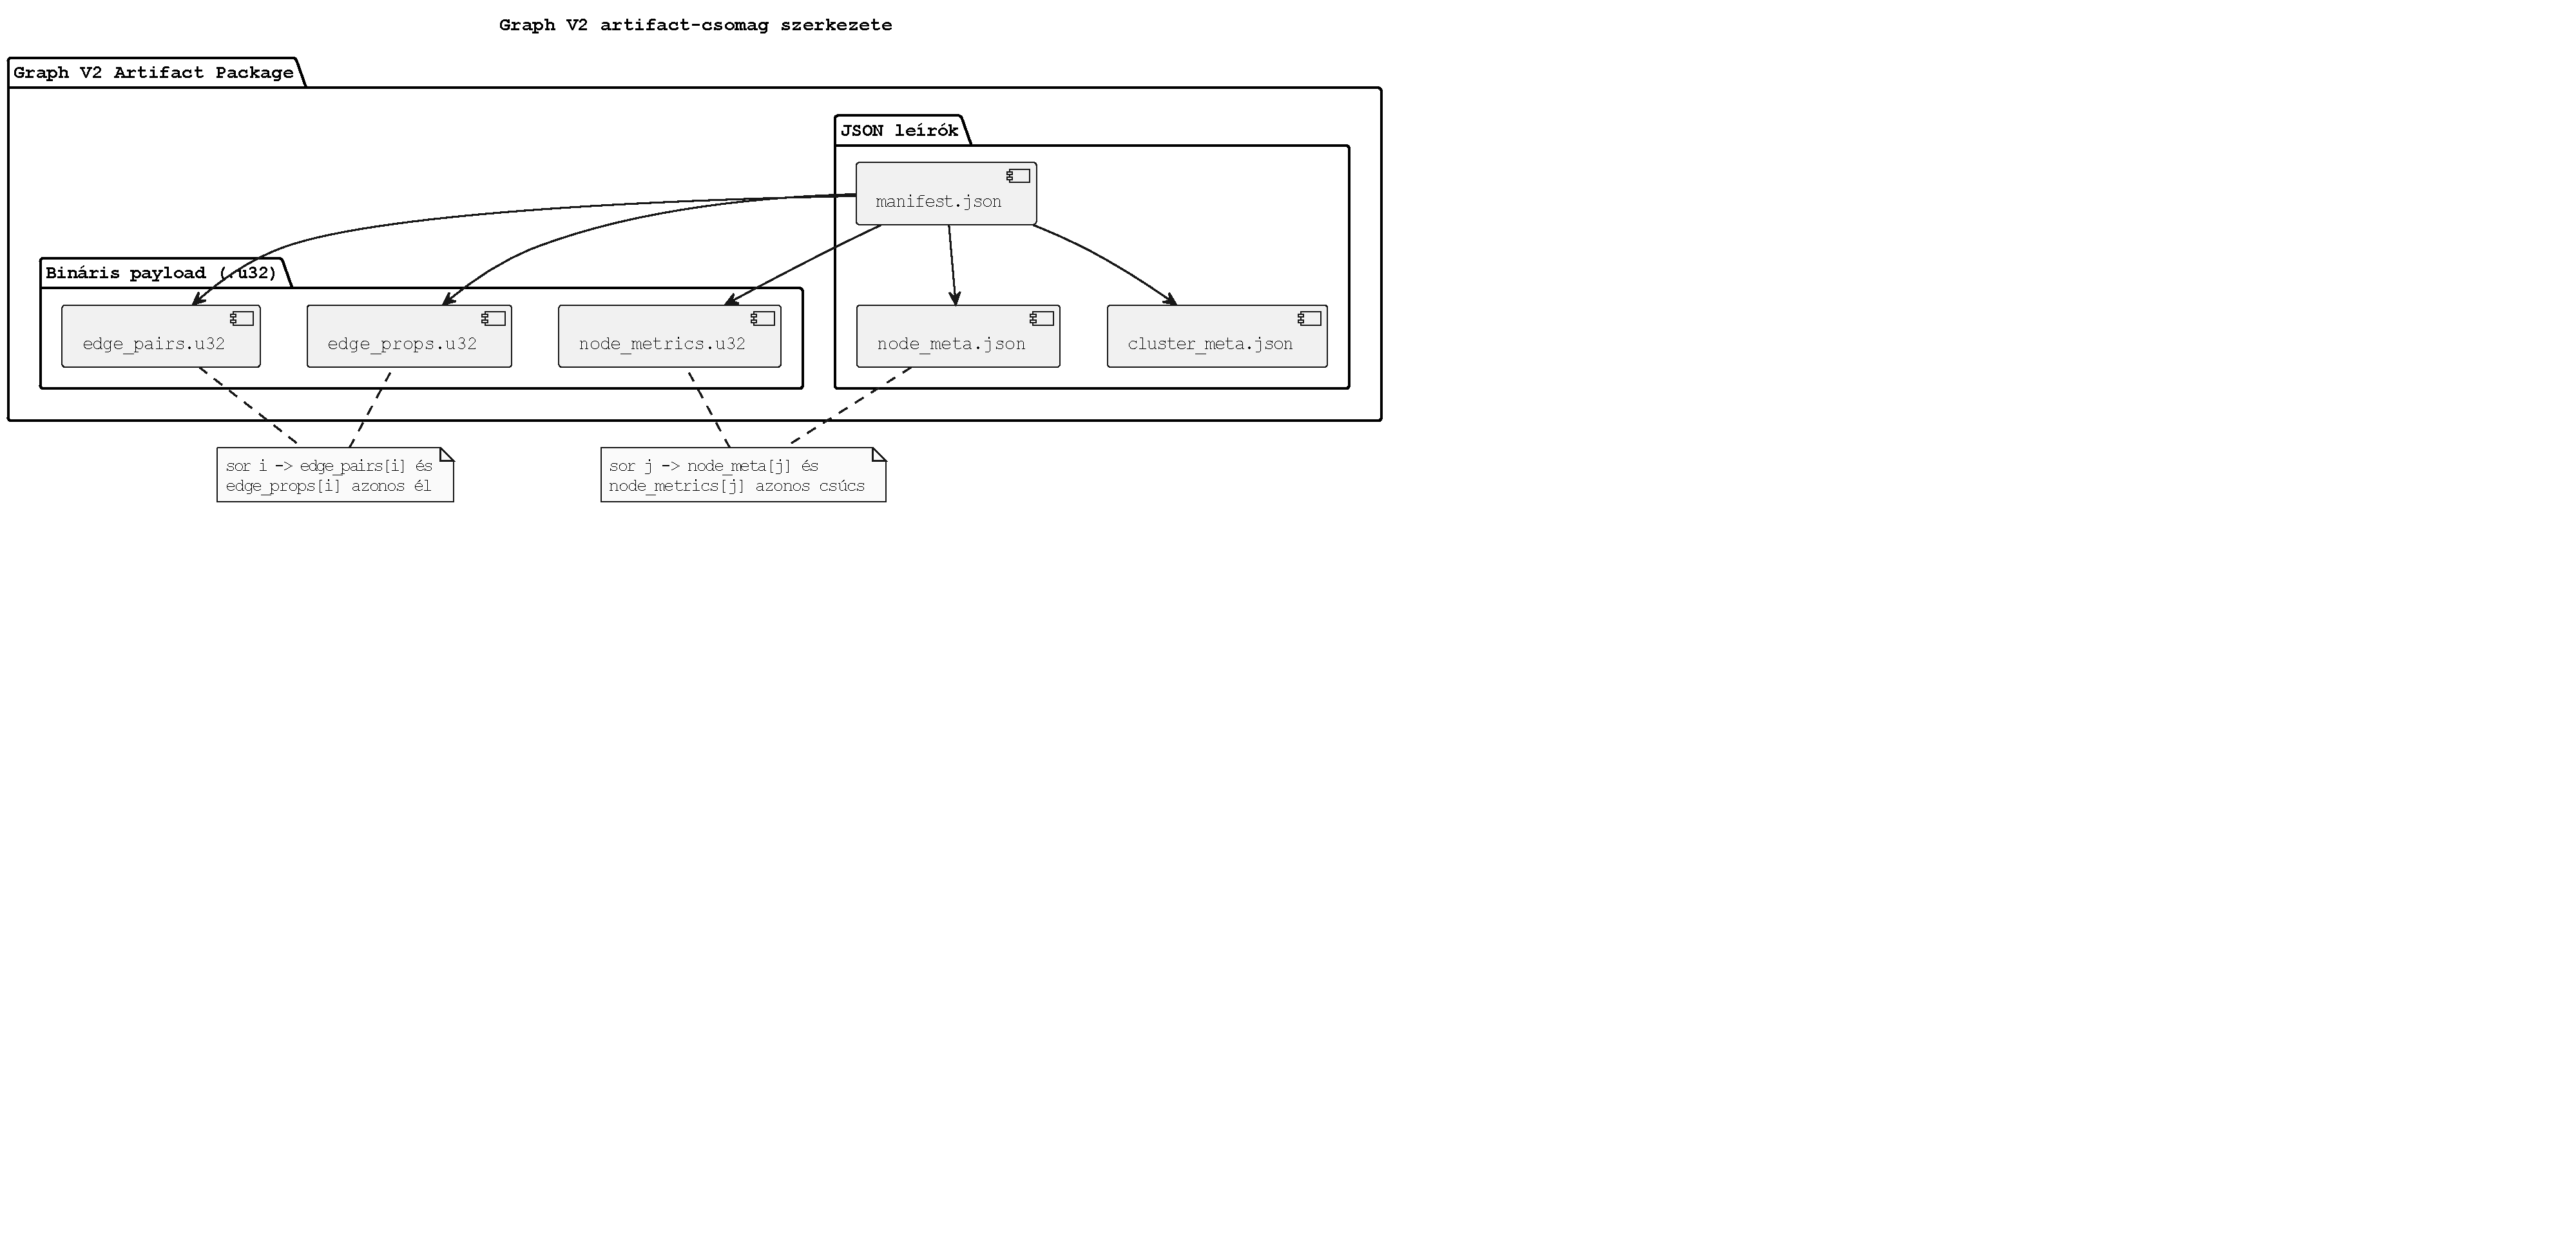
\includegraphics[width=\textwidth,height=0.82\textheight,keepaspectratio]{graph artifact components.pdf}
\caption{A Graph V2 pipeline bináris és JSON artifact-fájljainak szerkezete. A diagram a \texttt{graph-v2-artifact-structure.puml} forrás alapján különíti el a JSON leírókat (\texttt{manifest.json}, \texttt{node\_meta.json}, \texttt{cluster\_meta.json}) és a little-endian \texttt{.u32} bináris payloadokat (\texttt{edge\_pairs.u32}, \texttt{edge\_props.u32}, \texttt{node\_metrics.u32}). A \texttt{manifest.json} tartalmazza a csúcs-, él- és klaszterszámokat, míg a párhuzamos indexelés biztosítja, hogy az azonos sorszámú metadata- és metric-sor ugyanarra a csúcsra, illetve az azonos sorszámú edge-pair és edge-prop rekord ugyanarra az élre vonatkozzon.}
\end{figure}

A bináris formátumok (\texttt{.u32}) célja a betöltési teljesítmény: a frontend nem kénytelen JSON-parszolást végezni a csúcs- és élmutatókon; a bináris buffer közvetlenül beolvasható a WebGL renderelési pipeline-ba. Ez különösen a nagyméretű flexset esetén kritikus.

\subsection{A summary.md mint gépi és emberi kontextus}

Minden Graph V2 generálás után a pipeline létrehozza a \texttt{summary.md} fájlt, amely:

\begin{itemize}
    \item tartalmazza az összes kulcsmutatót (meccszám, csúcsszám, élszám, arányok, átlagos élsúly);
    \item dokumentálja a konstrukciós szemantikát (support-küszöb, tie-policy, klaszterméret-korlát);
    \item ML-szempontú feature-térképet biztosít a csomópont-, él- és klaszterszintű elemzési jelöltekhez;
    \item listázza a top bridge-orbit klasztereket;
    \item tartalmaz interpretációs korlátokat és javasolt elemzési irányokat.
\end{itemize}

Ennek a fájlnak kettős szerepe van: egyrészt fejlesztői ellenőrzőpontként működik (újragenerálásnál gyorsan ellenőrizhető, hogy a számok konzisztensek-e), másrészt gépi kontextusként is felhasználható - pontosan az a célba vett felhasználási mód, amelynek keretében a jelen dolgozat analitikai fejezetei is készültek.

\subsection{Verziókezelés és cache-érvénytelenítés}

A \texttt{graphBuilderVersion} mező (\texttt{graph-builder-v2.2}) explicit jelölője az artifaktum-csomag kompatibilitásának. Ha az algoritmus vagy a séma változik, a verzió frissítése egyértelműen jelzi, hogy a korábban generált artifact-csomagok nem felelnek meg az új elvárásoknak, és újra kell generálni azokat.

A \texttt{generatedAtUnixMs} Unix-időbélyeg lehetővé teszi a dataset-változás utáni automatikus érvénytelenítés detektálását: ha a meccs-JSON fájlok újabbak, mint a generálási időbélyeg, a rendszer tudja, hogy az artifact elavult.

\section{A backend API-szerződés}

A Rust motor és a frontend közötti kommunikáció a Node.js Express szerver (\texttt{backend/server.js}) által közvetített HTTP-végpontokon keresztül zajlik. A szerver nem saját maga végzi a számításokat, hanem a Rust folyamat stdin/stdout csatornáján továbbítja a kéréseket.

\subsection{Az aktuális főbb végpontok}

\begin{table}[H]
\centering
\caption{A backend API főbb végpontjai és szerepük}
\small
\begin{tabularx}{\textwidth}{>{\ttfamily\raggedright\arraybackslash}p{5.5cm} >{\raggedright\arraybackslash}X}
\toprule
\textbf{Végpont} & \textbf{Funkció} \\
\midrule
POST /api/pathfinder & Útvonalkeresési kérés (BFS/Dijkstra/A*/kétirányú) \\
POST /api/signed-balance & Kísérleti strukturális egyensúly-elemzés, nem fő felhasználói útvonal \\
POST /api/assortativity & Asszortativitás számítás \\
POST /api/betweenness-centrality & Brandes-betweenness futtatás \\
POST /api/balance-sweep & Kísérleti előjelprojekciós érzékenységi sweep \\
POST /api/assortativity-significance & Permutációs szignifikanciateszt \\
GET /api/graph-snapshot & Futásidejű gráfállapot-összefoglalás \\
GET /api/engine-spec & A Rust motor specifikációjának lekérése \\
GET /api/datasets & Elérhető datasetek listája \\
POST /api/switch-dataset & Dataset-váltás (Rust réteg újraindítással) \\
\bottomrule
\end{tabularx}
\normalsize
\end{table}

\subsection{Dataset-propagáció}

A dataset-váltás (\texttt{/api/switch-dataset}) nem csupán egy konfigurációs bit megváltoztatása. A Rust motor a dataset-specifikáció alapján teljes újraépítést végez: betölti az adott dataset meccs-JSON-jait, klasztereit és játékosprofilját, majd újraszámolja a landmark-távolságokat és a min-cost táblát. Ez az operáció jellemzően néhány másodpercig tart (a flexset esetén a futásidejű gráfépítés a teljes 4980 meccssel és 5741 csúccsal dolgozik).

Ez a közvetlen következménye annak az architektúrális döntésnek, hogy a Rust motor \emph{stateful}: nem minden kérésre, hanem beinduláskor (vagy dataset-váltáskor) tölti be a gráfot. Ez teljesítményi szempontból hasznos - nem kell minden egyes kérés előtt újraépíteni a gráfot -, de azt is jelenti, hogy a gráfállapot egy adott dataset-pillanathoz van kötve.

\subsection{A JSON-alapú kérés-válasz protokoll}

A Rust motor stdin-ről olvas egy JSON-objektumot (a kérés), majd stdout-ra ír egy JSON-objektumot (a válasz). A Node.js szerveroldal ezt a kommunikációt aszinkron Promisként kezeli. Ez a prototokol-tervzés egyszerű és debuggolható: a Rust motor tesztelható önállóan is, CLI eszközként, anélkül hogy a HTTP-szerver futna. A Node.js kizárólag a hálózati integrációért és a dataset-kezelésért felel.

\chapter{A strukturális egyensúly mint módszertani határeset}

\section{Miért került le a fő eredmények közül?}

A projektben elkészült signed-balance implementáció nem hibás algoritmus. A \texttt{signed\_balance.rs} modul determinisztikusan előállít egy előjeles egyszerű gráfot, teljesen összekapcsolt triádokat enumerál, majd a Heider--Cartwright--Harary-féle szabály szerint osztályozza őket. A visszaminősítés oka nem technikai, hanem szemantikai: a League of Legends matchmaking adataiban az ellenfélként való ismételt találkozás nem elég erős bizonyíték negatív társas kötésre.

Formálisan a projekció működik:

\begin{itemize}
    \item az \texttt{allyWeight} dominanciája pozitív élként kezelhető, mert a Flex Queue-ban a visszatérő csapattársi viszony részben szándékolt együttjátszást is tükrözhet;
    \item az \texttt{enemyWeight} dominanciája technikailag negatív élként jelölhető, de ez nem azonos ellenségességgel, rivalizálással vagy elutasítással;
    \item a döntetlen-kezelés, a minimum support és a triádenumerálás auditálható és újrafuttatható;
    \item a kapott arányok ezért inkább a választott projekció viselkedését mutatják, nem pedig bizonyított társas egyensúlyt.
\end{itemize}

\section{Az enemy-él szemantikai problémája}

A strukturális egyensúlyelmélet eredeti közege pozitív és negatív társas viszonyokra épül: barátságra, ellenszenvre, bizalomra, elutasításra vagy hasonló relációkra. A jelen projektben azonban egy enemy-él csak azt jelenti, hogy két játékos többször került egymással szembe, mint egy csapatba.

Ez sokféle okból történhet:

\begin{itemize}
    \item hasonló MMR-sávban játszanak;
    \item hasonló napszakban queue-znak;
    \item a Master$+$ Flex Queue aktív játékospoolja kicsi;
    \item a matchmaking ismételten ugyanazokat a játékosokat osztja ellenkező oldalra;
    \item a stabil premade-csoportok miatt a külső játékosok gyakrabban ellenfélként jelennek meg;
    \item az adatgyűjtési stratégia felerősítheti az ismétlődő találkozásokat.
\end{itemize}

Ezek közül egyik sem követeli meg, hogy a két játékos között negatív társas kapcsolat legyen. Ezért az \texttt{enemyWeight} negatív signed-network élként való kezelése túl erős állítás lenne a dolgozat fő empirikus narratívájához.

\section{Mit őriz meg a dolgozat?}

A signed-balance modul a repositoryban kísérleti opcióként megmaradhat, mert hasznos módszertani tanulságot ad: megmutatja, hogy egy formálisan elegáns gráfelméleti módszer hogyan válhat interpretációs szempontból gyengévé, ha az él szemantikája nem felel meg az elmélet előfeltevéseinek. A magas balance-ratio ezért legfeljebb óvatossági példaként használható: a szám lehet stabil a választott projekció alatt, de önmagában nem bizonyít társas harmóniát vagy strukturális stabilitást.

A dolgozati termékből és a fő frontend bemutatási útvonalból ezért kikerül a Signed Balance oldal és a kombinált Signed Balance + Assortativity futtató. A backend/Rust implementáció megtartható, de a dolgozat fő pillérei a következők:

\begin{itemize}
    \item a \texttt{flexset} asszociatív core-periphery játékosgráfként való értelmezése;
    \item a \texttt{flexset} és \texttt{soloq} datasetek kontrollált összehasonlítása;
    \item az \texttt{opscore} és \texttt{feedscore} asszortativitási eredményei;
    \item a Graph V2 konstrukciós és vizualizációs pipeline;
    \item a Rust útvonalkeresés és Brandes-betweenness központiság.
\end{itemize}

\section{Módszertani tanulság}

A visszaminősítés erősíti, nem gyengíti a dolgozatot. A dolgozat így nem azt állítja, hogy minden elegáns gráfelméleti modell automatikusan átültethető játékos-telemetriára, hanem azt, hogy az adatkeletkezési mechanizmust minden esetben össze kell vetni a választott modell előfeltevéseivel. A signed-balance esetben a formális számítás helyes, de a negatív él jelentése nem elég erős. Emiatt az elemzés határesetként marad: implementált, dokumentált, de nem fő bizonyíték.

\chapter{Gráfanalitikai eredmények: asszortativitás és betweenness centralitás}

A PremadeGraph két fő gráfanalitikai modulja az asszortativitás és a Brandes-féle betweenness centralitás. Mindkettő a Rust futtatókörnyezetben van implementálva, a frontend dedikált analitikai oldalakon jeleníti meg az eredményeket. Az asszortativitás azt vizsgálja, hogy az összekapcsolt játékosok hasonló teljesítményprofilhoz tartoznak-e; a betweenness centralitás azt méri, hogy egyes csomópontok hány legrövidebb úton helyezkednek el, tehát topológiai bróker-szerepet töltenek-e be.

\section{Asszortativitás}

\subsection{A számítási definíció}

A jelenlegi implementáció numerikus asszortativitást számol Pearson-korreláció formájában. Ha az él egyik végpontján mért értékeket $x_i$, a másik végpontén mért értékeket pedig $y_i$ jelöli, akkor az együttható:

\begin{equation}
r = \frac{\sum_i (x_i-\bar{x})(y_i-\bar{y})}{\sqrt{\sum_i (x_i-\bar{x})^2}\sqrt{\sum_i (y_i-\bar{y})^2}}
\end{equation}

Az irányítatlan éleket az implementáció mindkét endpoint-orientációval figyelembe veszi a Pearson-akkumulációban, mert az élnek nincs természetes iránya, és a két végpont tulajdonságpárja szimmetrikusan járul hozzá a korrelációhoz. A modul emellett külön számolja az alacsony támogatás, a hiányzó score és a túl rövid játékostörténet miatt kihagyott éleket, így az asszortativitási eredmény nem feketedoboz-korreláció, hanem dokumentált mintaképzési folyamat eredménye.

\begin{figure}[h]
\centering
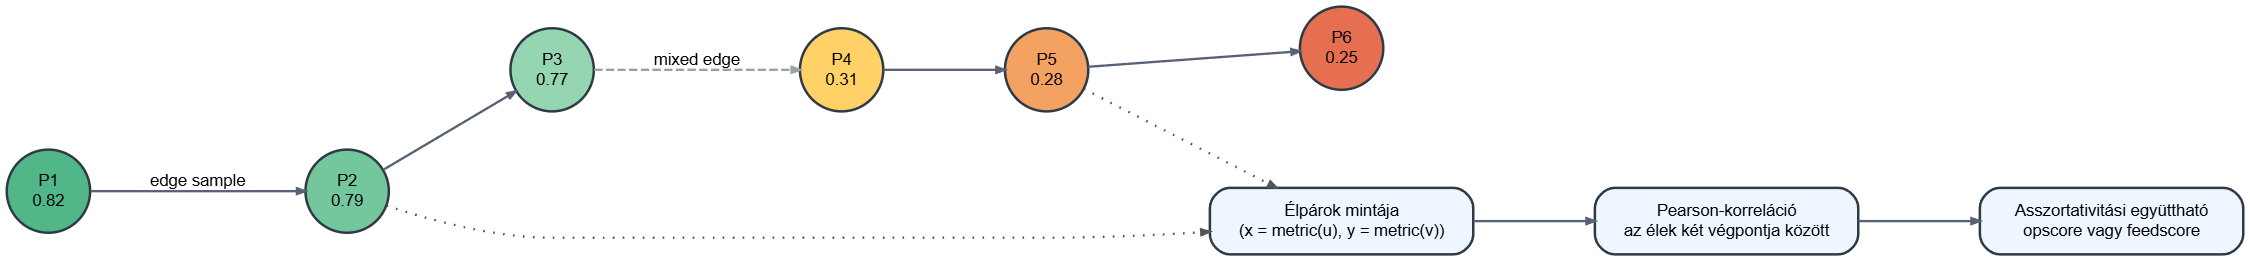
\includegraphics[width=0.92\textwidth]{assets/diagrams/thesis_assortativity_graphviz.png}
\caption{Az asszortativitás él-végponti értelmezése: az összekapcsolt játékospárok metrikaértékei Pearson-korrelációként kerülnek összesítésre.}
\label{fig:assortativity-graphviz-overview}
\end{figure}

\begin{figure}[H]
\centering
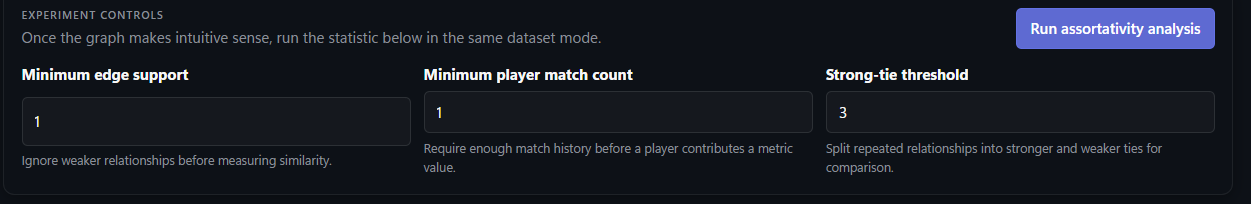
\includegraphics[width=0.98\textwidth,height=0.30\textheight,keepaspectratio]{assortavity-controls.png}
\caption{Az asszortativitási kísérlet frontend kontrolljai. A képen a minimum éltámogatás, a minimum játékos-meccsszám és az erős kapcsolat küszöbe látható; a bemutatott futtatásokban ezek rendre 1, 1 és 3 értékkel szerepelnek.}
\end{figure}

\begin{figure}[H]
\centering
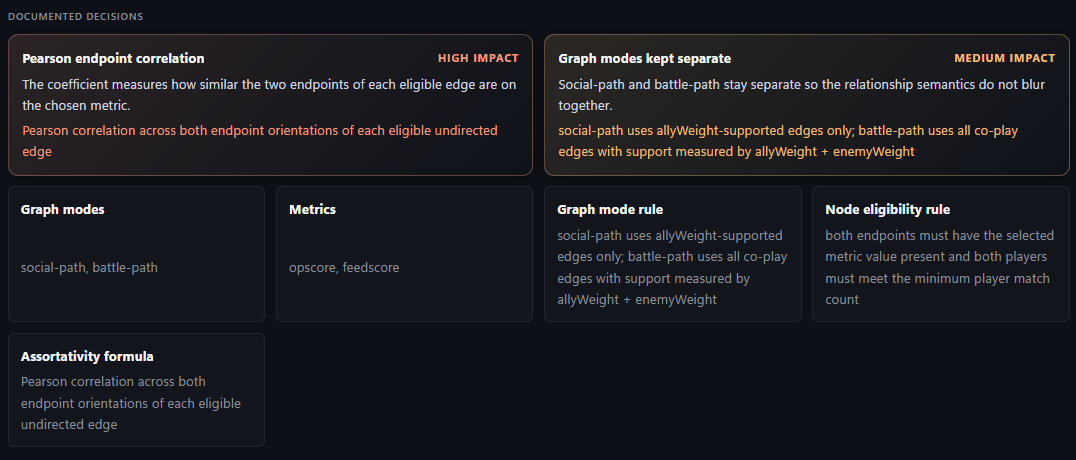
\includegraphics[width=0.98\textwidth,height=0.48\textheight,keepaspectratio]{assortavity-documented-desicions.png}
\caption{A frontend által megjelenített dokumentált módszertani döntések. A képernyő rögzíti, hogy Pearson endpoint-korrelációt használunk, a \textit{social-path} és \textit{battle-path} módokat külön kezeljük, a metrikák az \textit{opscore} és \textit{feedscore}, és csak azok a végpontok maradnak a mintában, amelyekhez érvényes metrika és elegendő meccstörténet tartozik.}
\end{figure}

\subsection{Él-végponti minta kiválasztása}

A Pearson-korreláció az élek között számítódik. Az implementáció az összes élt végigfuttatja az aktuális gráfmódnak megfelelő szűrőn, majd minden élhez lekérdezi az egyik és a másik végpont \textit{opscore} vagy \textit{feedscore} értékét. Ha bármelyik score hiányzik, vagy ha valamelyik játékos \textit{match\_count} értéke a minimum alá esik, az él kiesik. A maradék élek score-párjai képezik az akkumulált vektorokat. Ez a szűrés olyan mintahalmazt eredményez, amely az erős kapcsolatok körül tömörödik: az asszortativitás nem „mindent figyelembe vevő" globális mérőszám, hanem a releváns kapcsolathálózat szerkezeti tulajdonsága.

\subsection{Gráfmód-specifikus él-súlyozás}

A gráfmód alapján az él-súlyozás a következőképpen alakul:

\begin{equation}
w(u,v) = \begin{cases}
\textit{ally\_weight} & \text{ha } \textit{social-path} \\
\textit{total\_matches} & \text{ha } \textit{battle-path}
\end{cases}
\end{equation}

A \textit{social-path} módban csak a szövetségesi kapcsolatok sugallják az él meglétét; a \textit{battle-path} módban az összes ismétlődés (szövetséges és ellenséges) beszámít. Ez a különbség eltérő társas szerkezeti hipotéziseket tesztel: a social-path azt kérdezi, hogy a szövetségesi hálózatban csoportosulnak-e a hasonló teljesítmények, a battle-path pedig azt, hogy az összes ismétlődő kapcsolaton korrálnak-e.

\subsection{Bontások és hiányzó adat kezelése}

Az implementáció globális korreláción túl klaszteren belüli és klaszterek közötti, valamint erős és gyenge kapcsolatok szerinti bontást is képez. Ha a within-cluster érték magasabb, az a klasztertagok hasonló teljesítményprofilját jelzi; ha a between-cluster is magas, az asszortativitás klaszter-független tulajdonság. Hiányzó score-ok esetén az alapértelmezett \textit{skip} politika az óvatos választás: nem extrapolálunk hiányzó adatokra, így az eredmény az „amit ténylegesen tudunk" alapon számítódik.

\section{Asszortativitási eredmények}

\subsection{Flexset}

\begin{table}[H]
\centering
\caption{Asszortativitás - \textit{flexset}}
\begin{tabular}{llrr}
\toprule
\textbf{Gráfmód} & \textbf{Metrika} & \textbf{Korreláció} & \textbf{Mintaszám} \\
\midrule
\textit{social-path} & \textit{opscore} & 0.2346 & 61\,938 \\
\textit{social-path} & \textit{feedscore} & 0.1816 & 61\,938 \\
\textit{battle-path} & \textit{opscore} & 0.1461 & 179\,492 \\
\textit{battle-path} & \textit{feedscore} & $-0.0108$ & 179\,492 \\
\bottomrule
\end{tabular}
\end{table}

\begin{figure}[H]
\centering
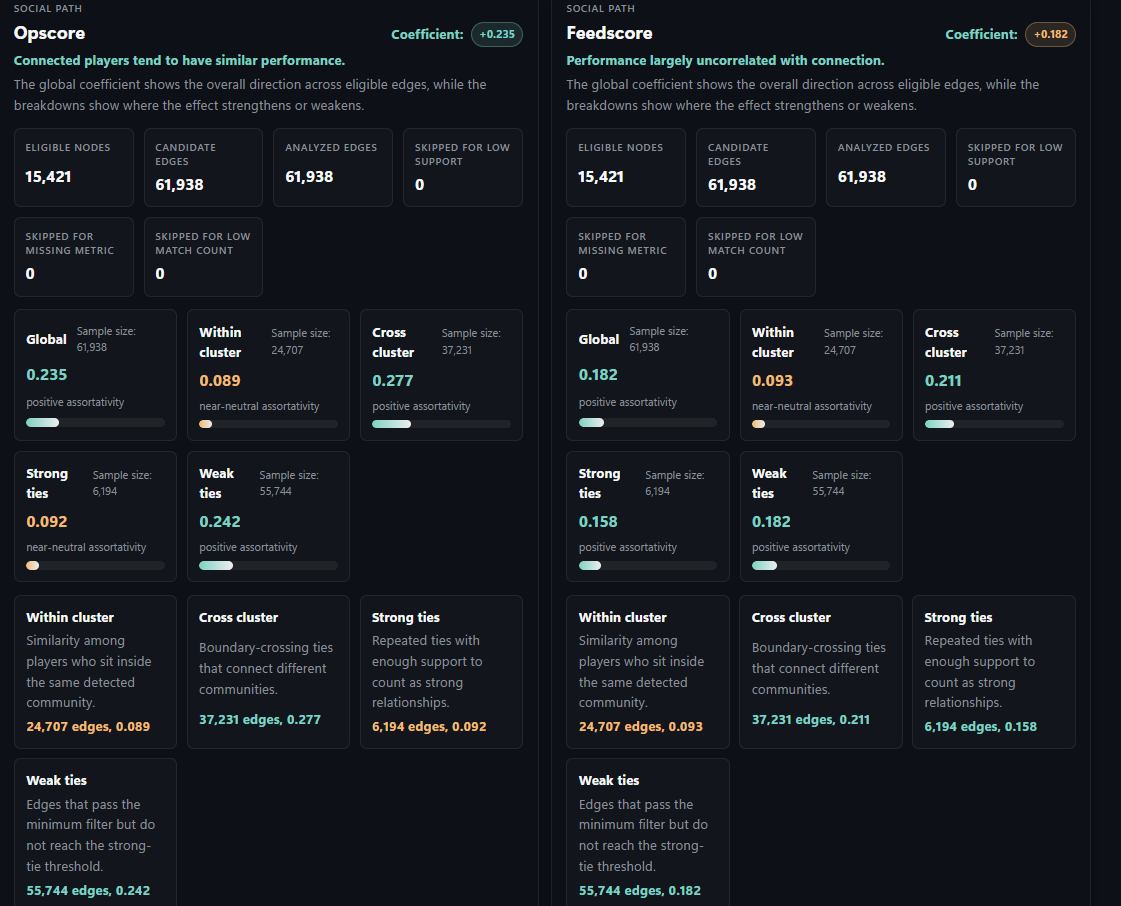
\includegraphics[width=0.98\textwidth,height=0.74\textheight,keepaspectratio]{f-assortavity-social-path-opfeedscore.png}
\caption{\textit{flexset} social-path asszortativitás \textit{opscore} és \textit{feedscore} szerint. A képen 15\,421 jogosult csomópont és 61\,938 elemzett él szerepel; a globális együttható \textit{opscore} esetén 0.235, \textit{feedscore} esetén 0.182. A bontások azt mutatják, hogy a kereszt-klaszter élek erősebb pozitív jelet adnak, mint a klaszteren belüli élek, miközben a gyenge kapcsolatok nagy mintaszámmal hordozzák a pozitív mintázatot.}
\end{figure}

\begin{figure}[H]
\centering
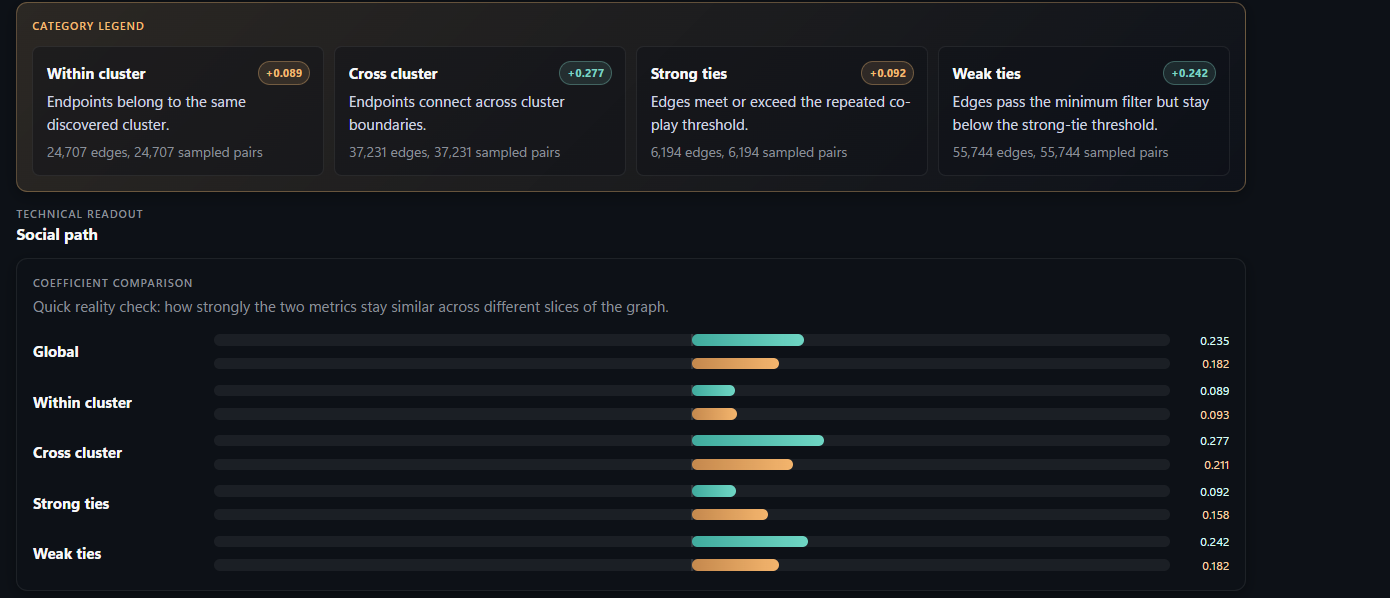
\includegraphics[width=0.98\textwidth,height=0.52\textheight,keepaspectratio]{f-assortavity-socialpath-readout.png}
\caption{\textit{flexset} social-path technikai readout. A sávos összehasonlítás a globális, within-cluster, cross-cluster, strong-tie és weak-tie bontásokat teszi egymás mellé; látható, hogy az \textit{opscore} minden bontásban pozitív, a \textit{feedscore} pedig social-path módban szintén pozitív marad.}
\end{figure}

\begin{figure}[H]
\centering
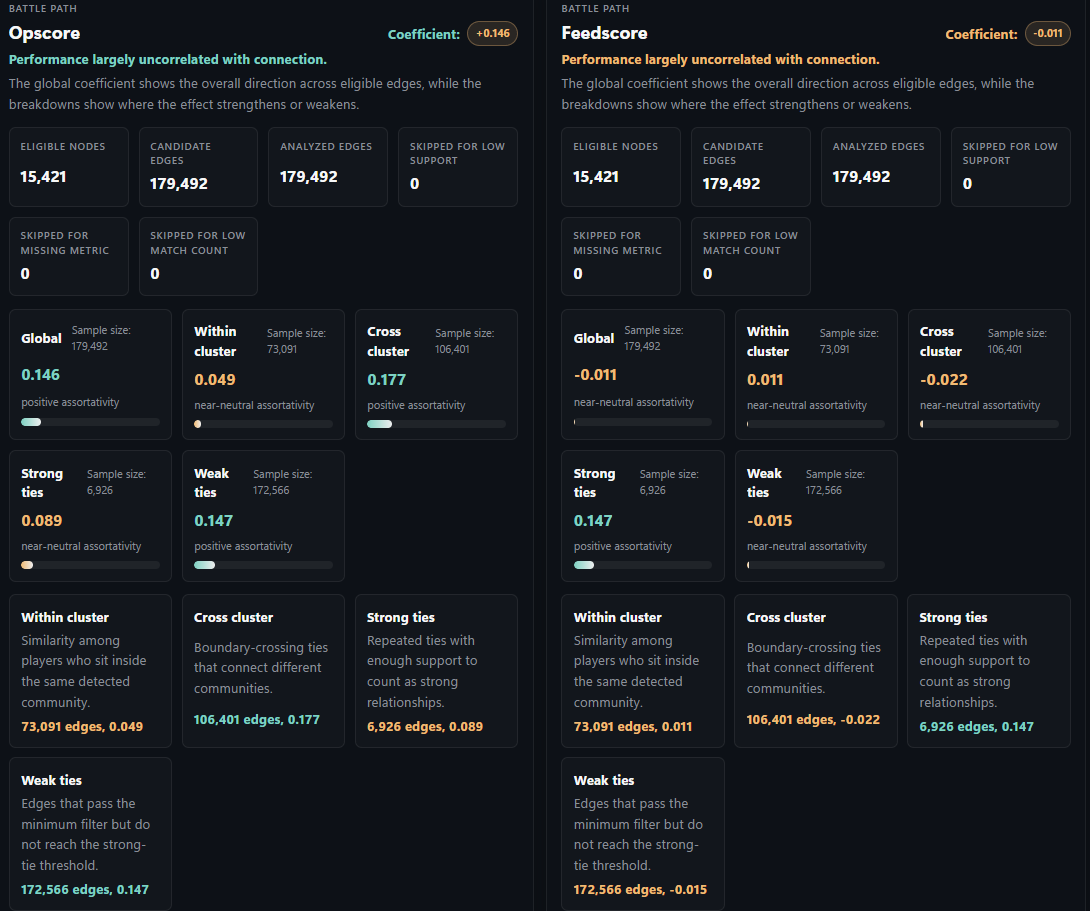
\includegraphics[width=0.98\textwidth,height=0.74\textheight,keepaspectratio]{f-assortavity-battle-path-opfeedscore.png}
\caption{\textit{flexset} battle-path asszortativitás \textit{opscore} és \textit{feedscore} szerint. A képen ugyanaz a 15\,421 jogosult csomópont, de már 179\,492 elemzett él látható; a \textit{battle-path} mód több kapcsolatot vesz be, ezért az \textit{opscore} jel 0.146-ra gyengül, a \textit{feedscore} pedig gyakorlatilag nullára esik ($-0.011$).}
\end{figure}

\begin{figure}[H]
\centering
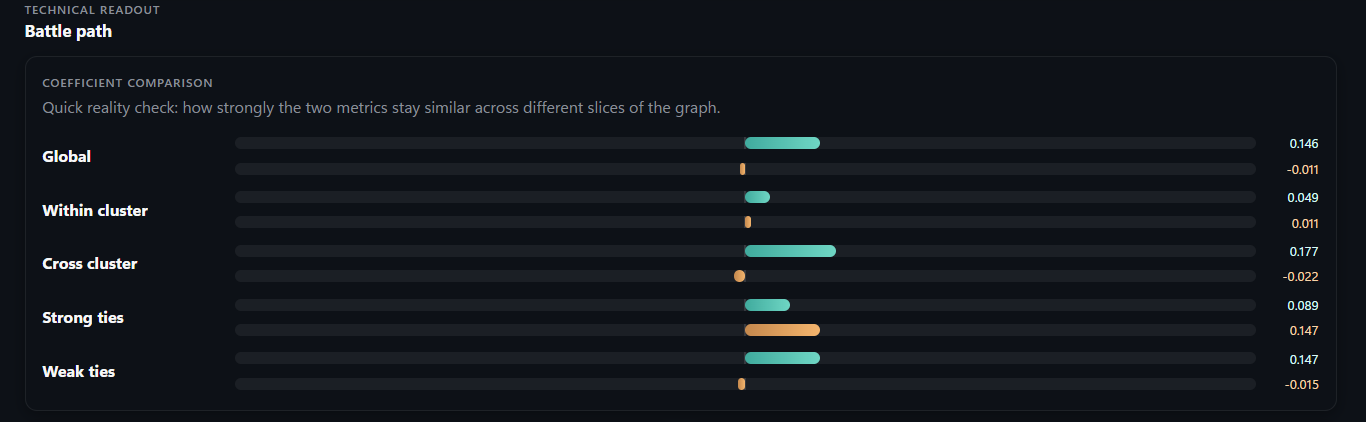
\includegraphics[width=0.98\textwidth,height=0.36\textheight,keepaspectratio]{f-assortavity-battlepath-readout.png}
\caption{\textit{flexset} battle-path technikai readout. A képernyőn az látszik, hogy a battle-path \textit{opscore} pozitív, de mérsékeltebb hasonlósági jelet ad, míg a \textit{feedscore} globálisan és a gyenge kapcsolatokon közel nulla vagy enyhén negatív.}
\end{figure}

\begin{figure}[H]
\centering
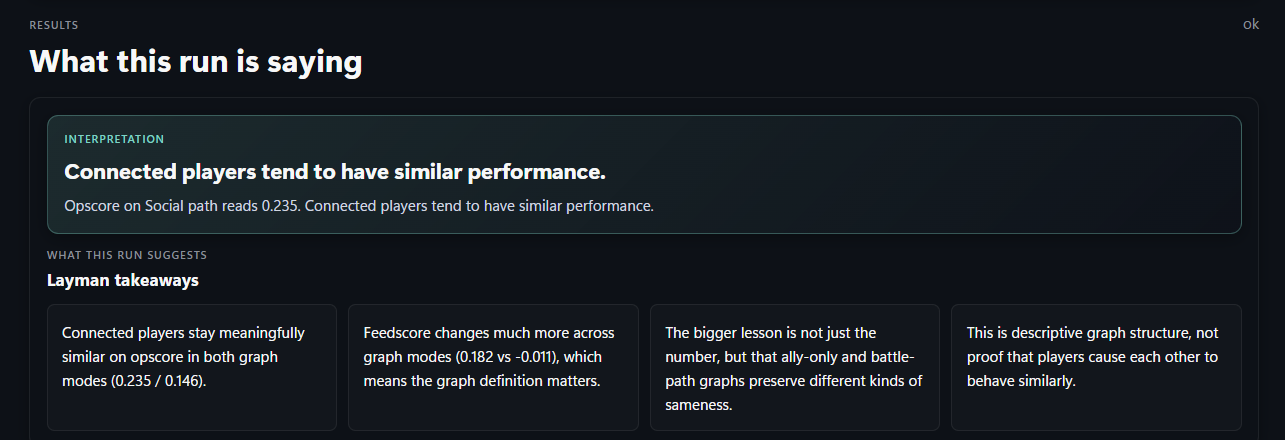
\includegraphics[width=0.98\textwidth,height=0.38\textheight,keepaspectratio]{f-assortavity-layman-takeaways.png}
\caption{\textit{flexset} közérthető frontend-összegzés. A képernyő azt emeli ki, hogy a kapcsolt játékosok \textit{opscore} szerint mindkét gráfmódban hasonlóbbak, a \textit{feedscore} viszont erősen gráfmód-függő; a következtetés leíró hálózati szerkezetről szól, nem oksági vagy pszichológiai állításról.}
\end{figure}

A \textit{flexset} legfontosabb tanulsága: a szövetségesi kapcsolatokra épülő social-path gráfban jelenik meg a legerősebb teljesítményhasonlósági jel. Ez illeszkedik ahhoz az értelmezéshez, hogy a Flex Queue nem pusztán véletlen matchmaking-minta. A cross-cluster \textit{opscore} érték magasabb, mint a within-cluster érték, tehát az asszortativitás nem egyszerűen a klaszterezés mellékterméke: a határkapcsolatokban is mérhető.

\subsection{SoloQ}

\begin{table}[H]
\centering
\caption{Asszortativitás - \textit{soloq}}
\begin{tabular}{llrr}
\toprule
\textbf{Gráfmód} & \textbf{Metrika} & \textbf{Korreláció} & \textbf{Mintaszám} \\
\midrule
\textit{social-path} & \textit{opscore} & 0.1750 & 37\,976 \\
\textit{social-path} & \textit{feedscore} & 0.1012 & 37\,976 \\
\textit{battle-path} & \textit{opscore} & 0.1625 & 84\,393 \\
\textit{battle-path} & \textit{feedscore} & $-0.0366$ & 84\,393 \\
\bottomrule
\end{tabular}
\end{table}

\begin{figure}[H]
\centering
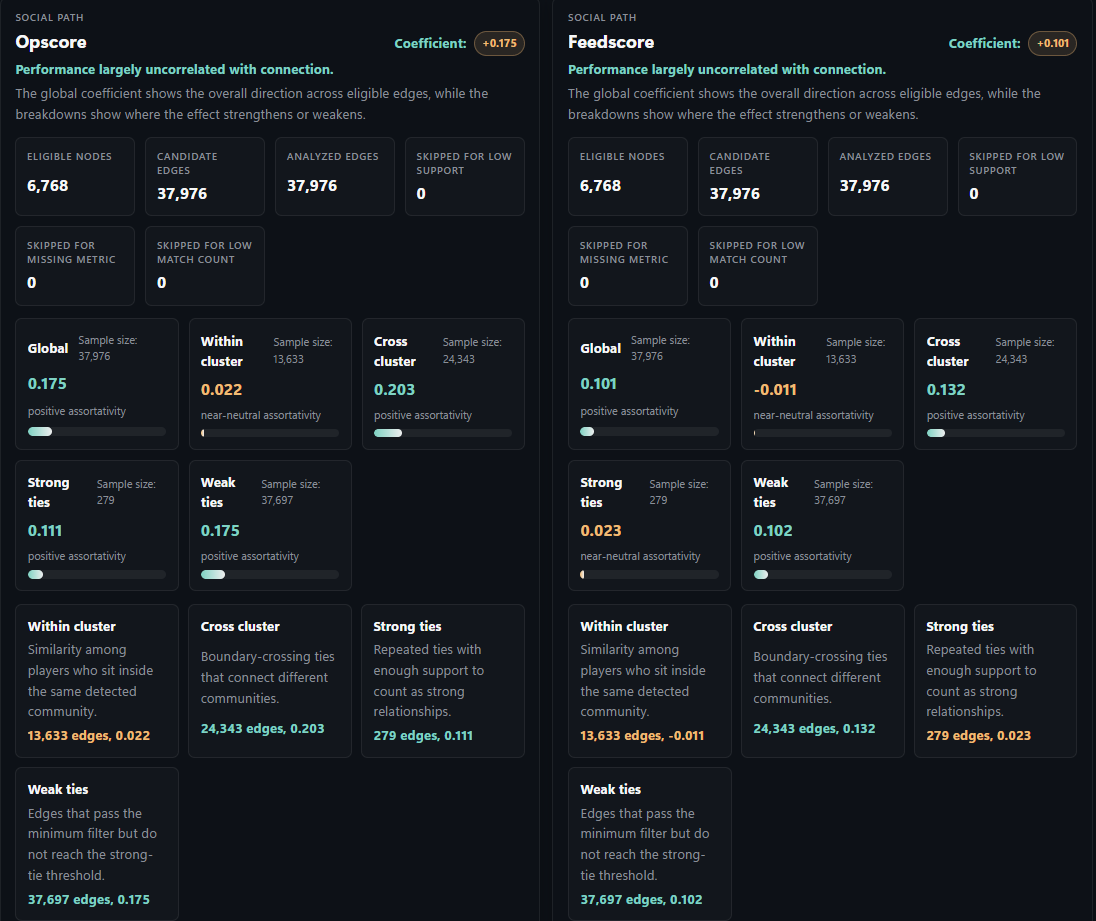
\includegraphics[width=0.98\textwidth,height=0.74\textheight,keepaspectratio]{sq-assortavity-social-path-opfeedscore.png}
\caption{\textit{soloq} social-path asszortativitás \textit{opscore} és \textit{feedscore} szerint. A képen 6\,768 jogosult csomópont és 37\,976 elemzett él szerepel; a globális együttható \textit{opscore} esetén 0.175, \textit{feedscore} esetén 0.101. A pozitív értékek megmaradnak, de gyengébbek, mint a \textit{flexset} social-path eredményei.}
\end{figure}

\begin{figure}[H]
\centering
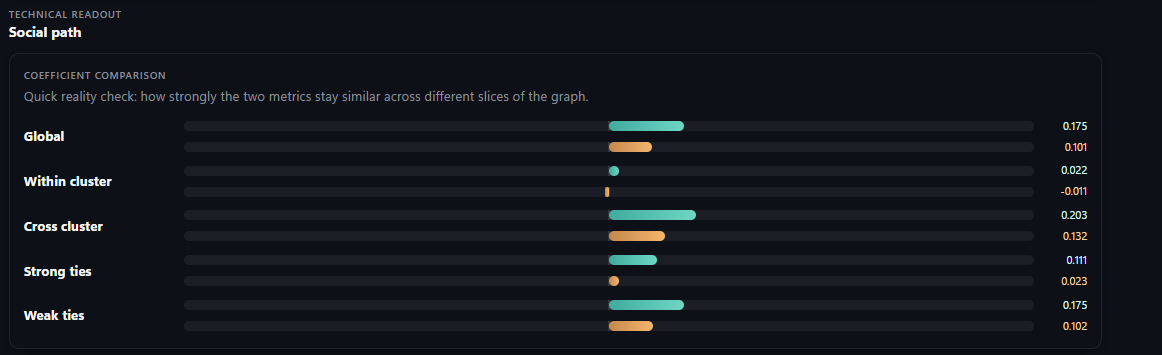
\includegraphics[width=0.98\textwidth,height=0.36\textheight,keepaspectratio]{sq-assortavity-socialpath-readout.png}
\caption{\textit{soloq} social-path technikai readout. A sávos nézet azt mutatja, hogy a cross-cluster bontás adja a legerősebb pozitív jelet, míg a within-cluster értékek közel semlegesek; a strong-tie minta különösen kicsi, ezért ebben a datasetben óvatosan értelmezendő.}
\end{figure}

\begin{figure}[H]
\centering
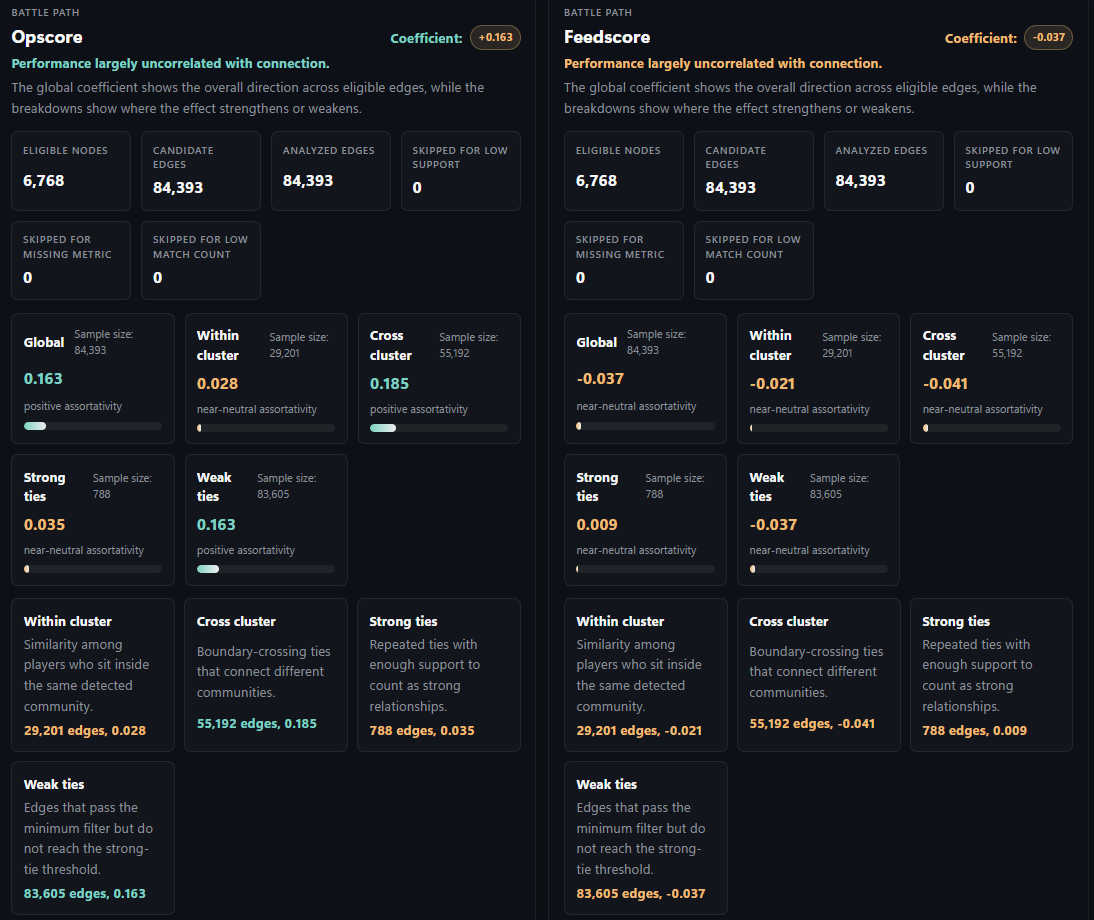
\includegraphics[width=0.98\textwidth,height=0.74\textheight,keepaspectratio]{sq-assortavity-battle-path-opfeedscore.png}
\caption{\textit{soloq} battle-path asszortativitás \textit{opscore} és \textit{feedscore} szerint. A képen 84\,393 elemzett él látható; az \textit{opscore} globálisan 0.163 marad, a \textit{feedscore} viszont $-0.037$ értékre fordul.}
\end{figure}

\begin{figure}[H]
\centering
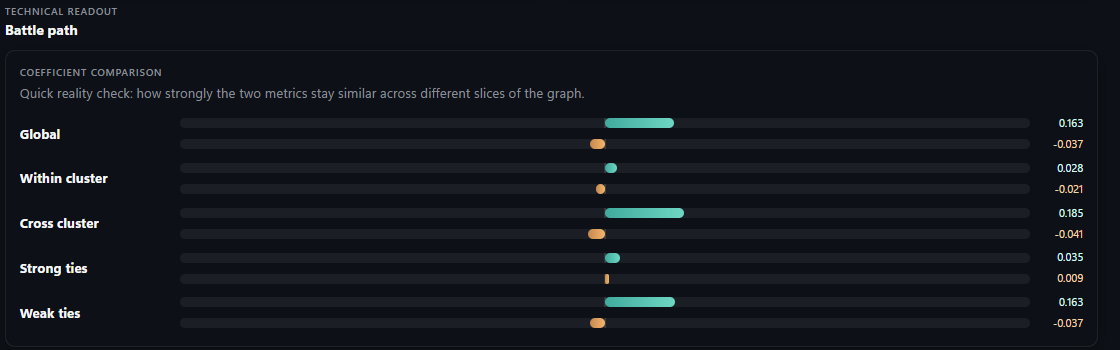
\includegraphics[width=0.98\textwidth,height=0.36\textheight,keepaspectratio]{sq-assortavity-battlepath-readout.png}
\caption{\textit{soloq} battle-path technikai readout. A képernyőn az \textit{opscore} pozitív, de mérsékelt értékei látszanak, míg a \textit{feedscore} globálisan, within-cluster és cross-cluster bontásban is negatív közeli értékeket vesz fel.}
\end{figure}

\begin{figure}[H]
\centering
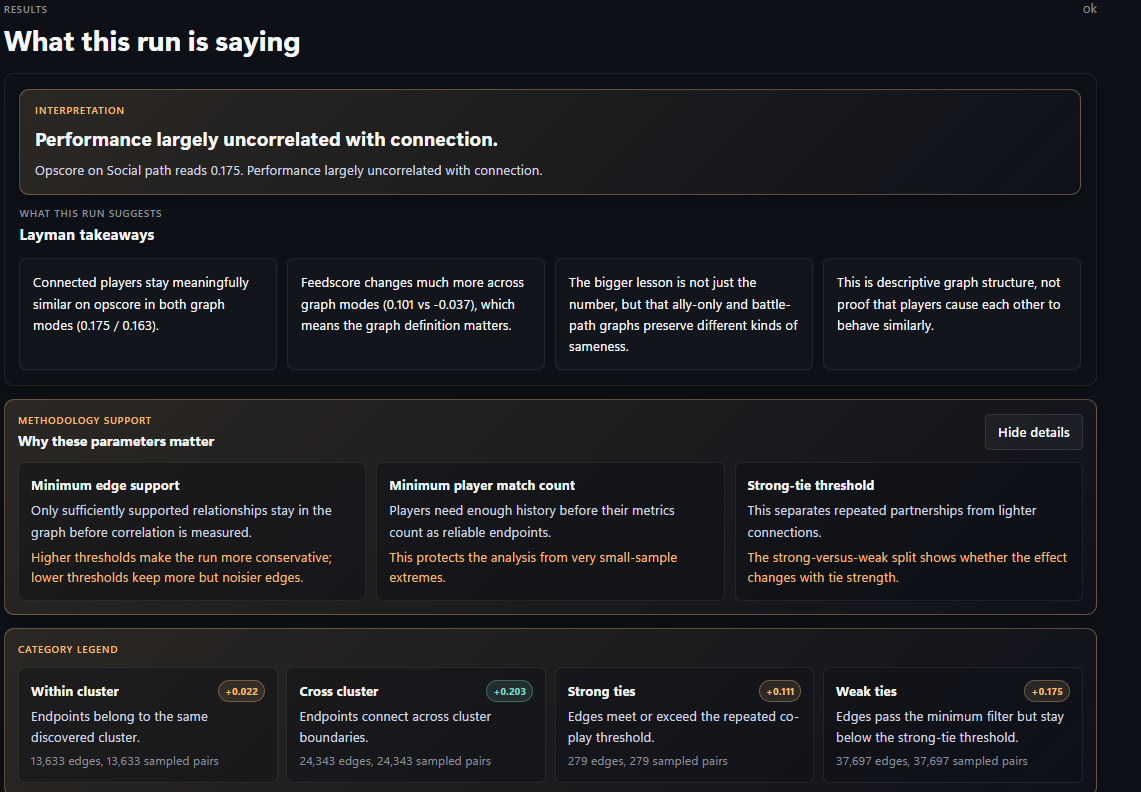
\includegraphics[width=0.98\textwidth,height=0.58\textheight,keepaspectratio]{sq-assortavity-layman-takeaways.png}
\caption{\textit{soloq} közérthető frontend-összegzés. A képernyő azt foglalja össze, hogy az \textit{opscore} hasonlóság mindkét gráfmódban megmarad, de a \textit{feedscore} jelentősen változik; a módszertani panel külön jelzi, hogy a minimum support, a minimum meccsszám és az erős kapcsolat küszöbe befolyásolja, mennyire konzervatív a futtatás.}
\end{figure}

A \textit{soloq} kontrollszerepe itt látszik: a pozitív \textit{opscore} asszortativitás nem tűnik el, tehát a teljesítményhasonlósági jel nem kizárólag Flex Queue sajátosság. Ugyanakkor a social-path érték alacsonyabb, a strong-tie minták kicsik, és a \textit{feedscore} battle-path módban negatív közeli eredményt ad. Ez azt támasztja alá, hogy a SoloQ inkább egyéni teljesítmény- és matchmaking-rekurrencia kontrollként értelmezhető, nem stabil premade-kapcsolati hálóként.

\subsection{Értelmezés}

Mindkét datasetben pozitív asszortativitás jelenik meg az \textit{opscore} mentén a \textit{social-path} módban, ami azt jelzi, hogy a szövetségesi kapcsolatokra épülő gráfban az összekapcsolt játékosok teljesítményprofilja nem véletlenszerűen keveredik. A \textit{feedscore} viselkedése jóval érzékenyebb a gráfmódra: social-path módban mindkét dataseten mérsékelt pozitív jel látható, de battle-path módban közel nullára esik (flexset: $-0.0108$, soloq: $-0.0366$). Az ellenfélkapcsolatok bevonásával a halálokon alapuló hibamutató elveszíti a társas-kapcsolati hasonlósági szerkezetet.

A flexset social-path \textit{opscore} asszortativitás (0.2346) magasabb, mint a soloq-é (0.1750), ami összhangban van azzal, hogy a Flex Queue erősebb visszatérő csapattársi szignált hoz létre. A battle-path mód mindkét datasetben lényegesen több élt vizsgál, de ez nem erősíti a korrelációt: a flexset esetén az élminta 61\,938-ról 179\,492-re nő, mégis csökken az \textit{opscore} asszortativitás és eltűnik a \textit{feedscore} jel. Több él nem automatikusan jobb bizonyíték, ha az élhalmaz szemantikája kevertebb.

Az \textit{opscore} minden vizsgált módban pozitív marad, a \textit{feedscore} nem; ez a kompozit mutató erőssége az egyszerűbb halálközpontú képlettel szemben. Nem azt állítjuk, hogy az \textit{opscore} objektív igazság, de empirikusan megmutatja, hogy a gráf és a score-réteg között érdemi kapcsolat van, és ez gráfmódváltáskor sem tűnik el. A gráfmód-érzékenység módszertani eredmény önmagában is: ha mindkét metrika minden módban azonos értéket adna, a gráfdefiníció nem hordozna önálló tartalmat. Az \textit{opscore} csökkenése battle-path módban és a \textit{feedscore} nullára esése azt mutatja, hogy a kapcsolatok szemantikája meghatározza a teljesítményhasonlóság mérhetőségét, és a két gráfmód megkülönböztetése empirikusan indokolt módszertani döntés.

A randomizációs szignifikanciateszt infrastruktúrája megvan a rendszerben, de a jelen dolgozatban a fő eredmények a közvetlenül ellenőrzött leíró és bontott futtatásokon alapulnak.

\section{Betweenness centralitás}

A bridge-orbit vizualizáció a Graph V2 pipeline-ból heurisztikus pontszámokkal (\textit{orbitScore}, \textit{orbitRadius}) azonosít egyes csomópontokat és klasztereket hidaknak. Ezek a mezők azonban vizuális heurisztikák: a kereszt-klaszter szövetségesi támasz, az összekötött klasztercsoport-szám és a tagszám kombinációján alapulnak, de nem ellenőrzik, hogy a jelölt csomópontok valóban a legtöbb legrövidebb útvonal metszéspontján helyezkednek-e el. A Brandes-féle betweenness centralitás éppen ezt az ellenőrzést teszi lehetővé: teljes gráfbejáráson alapul, nem becslésen.

\begin{figure}[h]
\centering
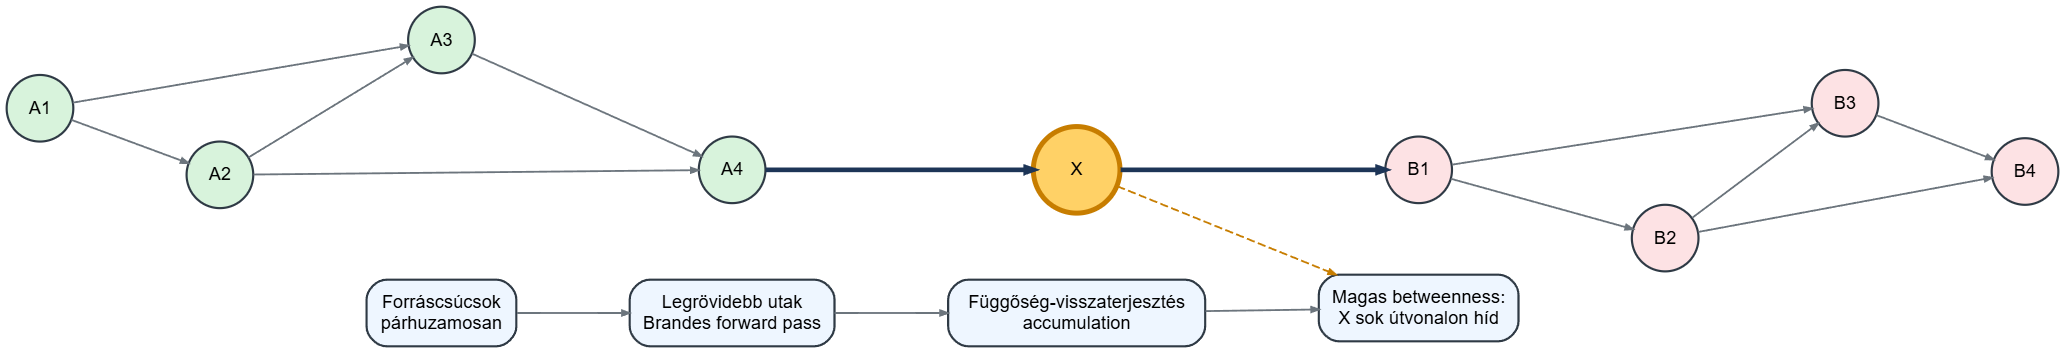
\includegraphics[width=0.92\textwidth]{assets/diagrams/thesis_brandes_bridge_graphviz.png}
\caption{A betweenness centralitás intuitív értelmezése: a hídcsomópont sok klaszterközi legrövidebb útvonalon jelenik meg, ezért magas Brandes-pontszámot kap.}
\label{fig:brandes-bridge-graphviz}
\end{figure}

\subsection{A Brandes-algoritmus}

A Brandes-algoritmus \cite{brandes2001} a hagyományos $O(n^3)$ komplexitású betweenness-számítást $O(nm)$-re csökkenti. Az ötlet az, hogy a csomópontonkénti legrövidebb-út fákat nem kell külön-külön tárolni: a forráscsomópontból induló BFS/Dijkstra-futtatás eredményéből egy visszaterjesztési lépésben kiszámítható az összes közötti részleges járulék. Forráscsomópontonként a lépések: Dijkstra/BFS futtatás a forrásból, amely kiszámolja a $\sigma[s][v]$ értéket (legrövidebb utak száma $s$-től $v$-ig) és a távolságokat; majd a feltehetős csomópontok fordított sorrendben kerülnek feldolgozásra, és minden $w$-re, amelynek előde $v$ a legrövidebb úton:

\begin{equation}
\delta[s][v] \mathrel{+}= \frac{\sigma[s][v]}{\sigma[s][w]} \cdot (1 + \delta[s][w])
\end{equation}

Irányítatlan gráfra az összes forrás feldolgozása után az eredmény felezése szükséges, mert minden $(s, t)$ és $(t, s)$ pár kétszer volt megszámlálva. A normalizálás az $(n-1)(n-2)/2$ maximális útvonalszámra vetít.

\subsection{Súlyozott mód és élköltség}

Súlyozott módban az élköltség:

\begin{equation}
c(u,v) = \left\lceil \frac{10^6}{\max(1, w(u,v))} \right\rceil
\end{equation}

ahol $w(u,v)$ az adott gráfmódnak megfelelő kapcsolaterősség (\textit{allyWeight} social-path módban, \textit{total\_matches} battle-path módban). A $10^6$-os skálázási konstans integeraritmetikai pontosságot biztosít: az egészre kerekített reciprok kis élsúlyoknál nagy, erős kapcsolatoknál kis költséget ad, és determinisztikus rendezési viselkedést biztosít a prioritásos sorban. Súlyozatlan módban az összes él ára $10^6$, ami egyenértékű az eredeti, súlyozatlan Brandes-bejárással.

\subsection{Párhuzamos végrehajtás}

A Rust \textit{rayon} könyvtára automatikus munkalopásos párhuzamosságot tesz lehetővé. A centralitás-modul a forráscsomópontok halmazát $k = \min(n, 4 \cdot \text{szálak száma})$ egyenlő méretű csomóponthalmazra osztja; minden halmazt egy párhuzamos rayon-feladatban dolgoz fel, ahol a lokális $\delta$ vektor független a többi résztől; az összegzés után a részeredmény-vektorok determinisztikusan összeadódnak. A forráscsomópontok rendezése és a chunk-határok rögzítése garantálja, hogy azonos input esetén mindig ugyanaz a kimenet; ezt a tesztcsomag explicit módon ellenőrzi.

A \ref{fig:parallel-brandes-activity}. ábra a párhuzamos Brandes-futtatás teljes aktivitásdiagramját mutatja, beleértve a forráscsomópontok elosztását és a determinisztikus redukciókat.

\begin{figure}[H]
\centering
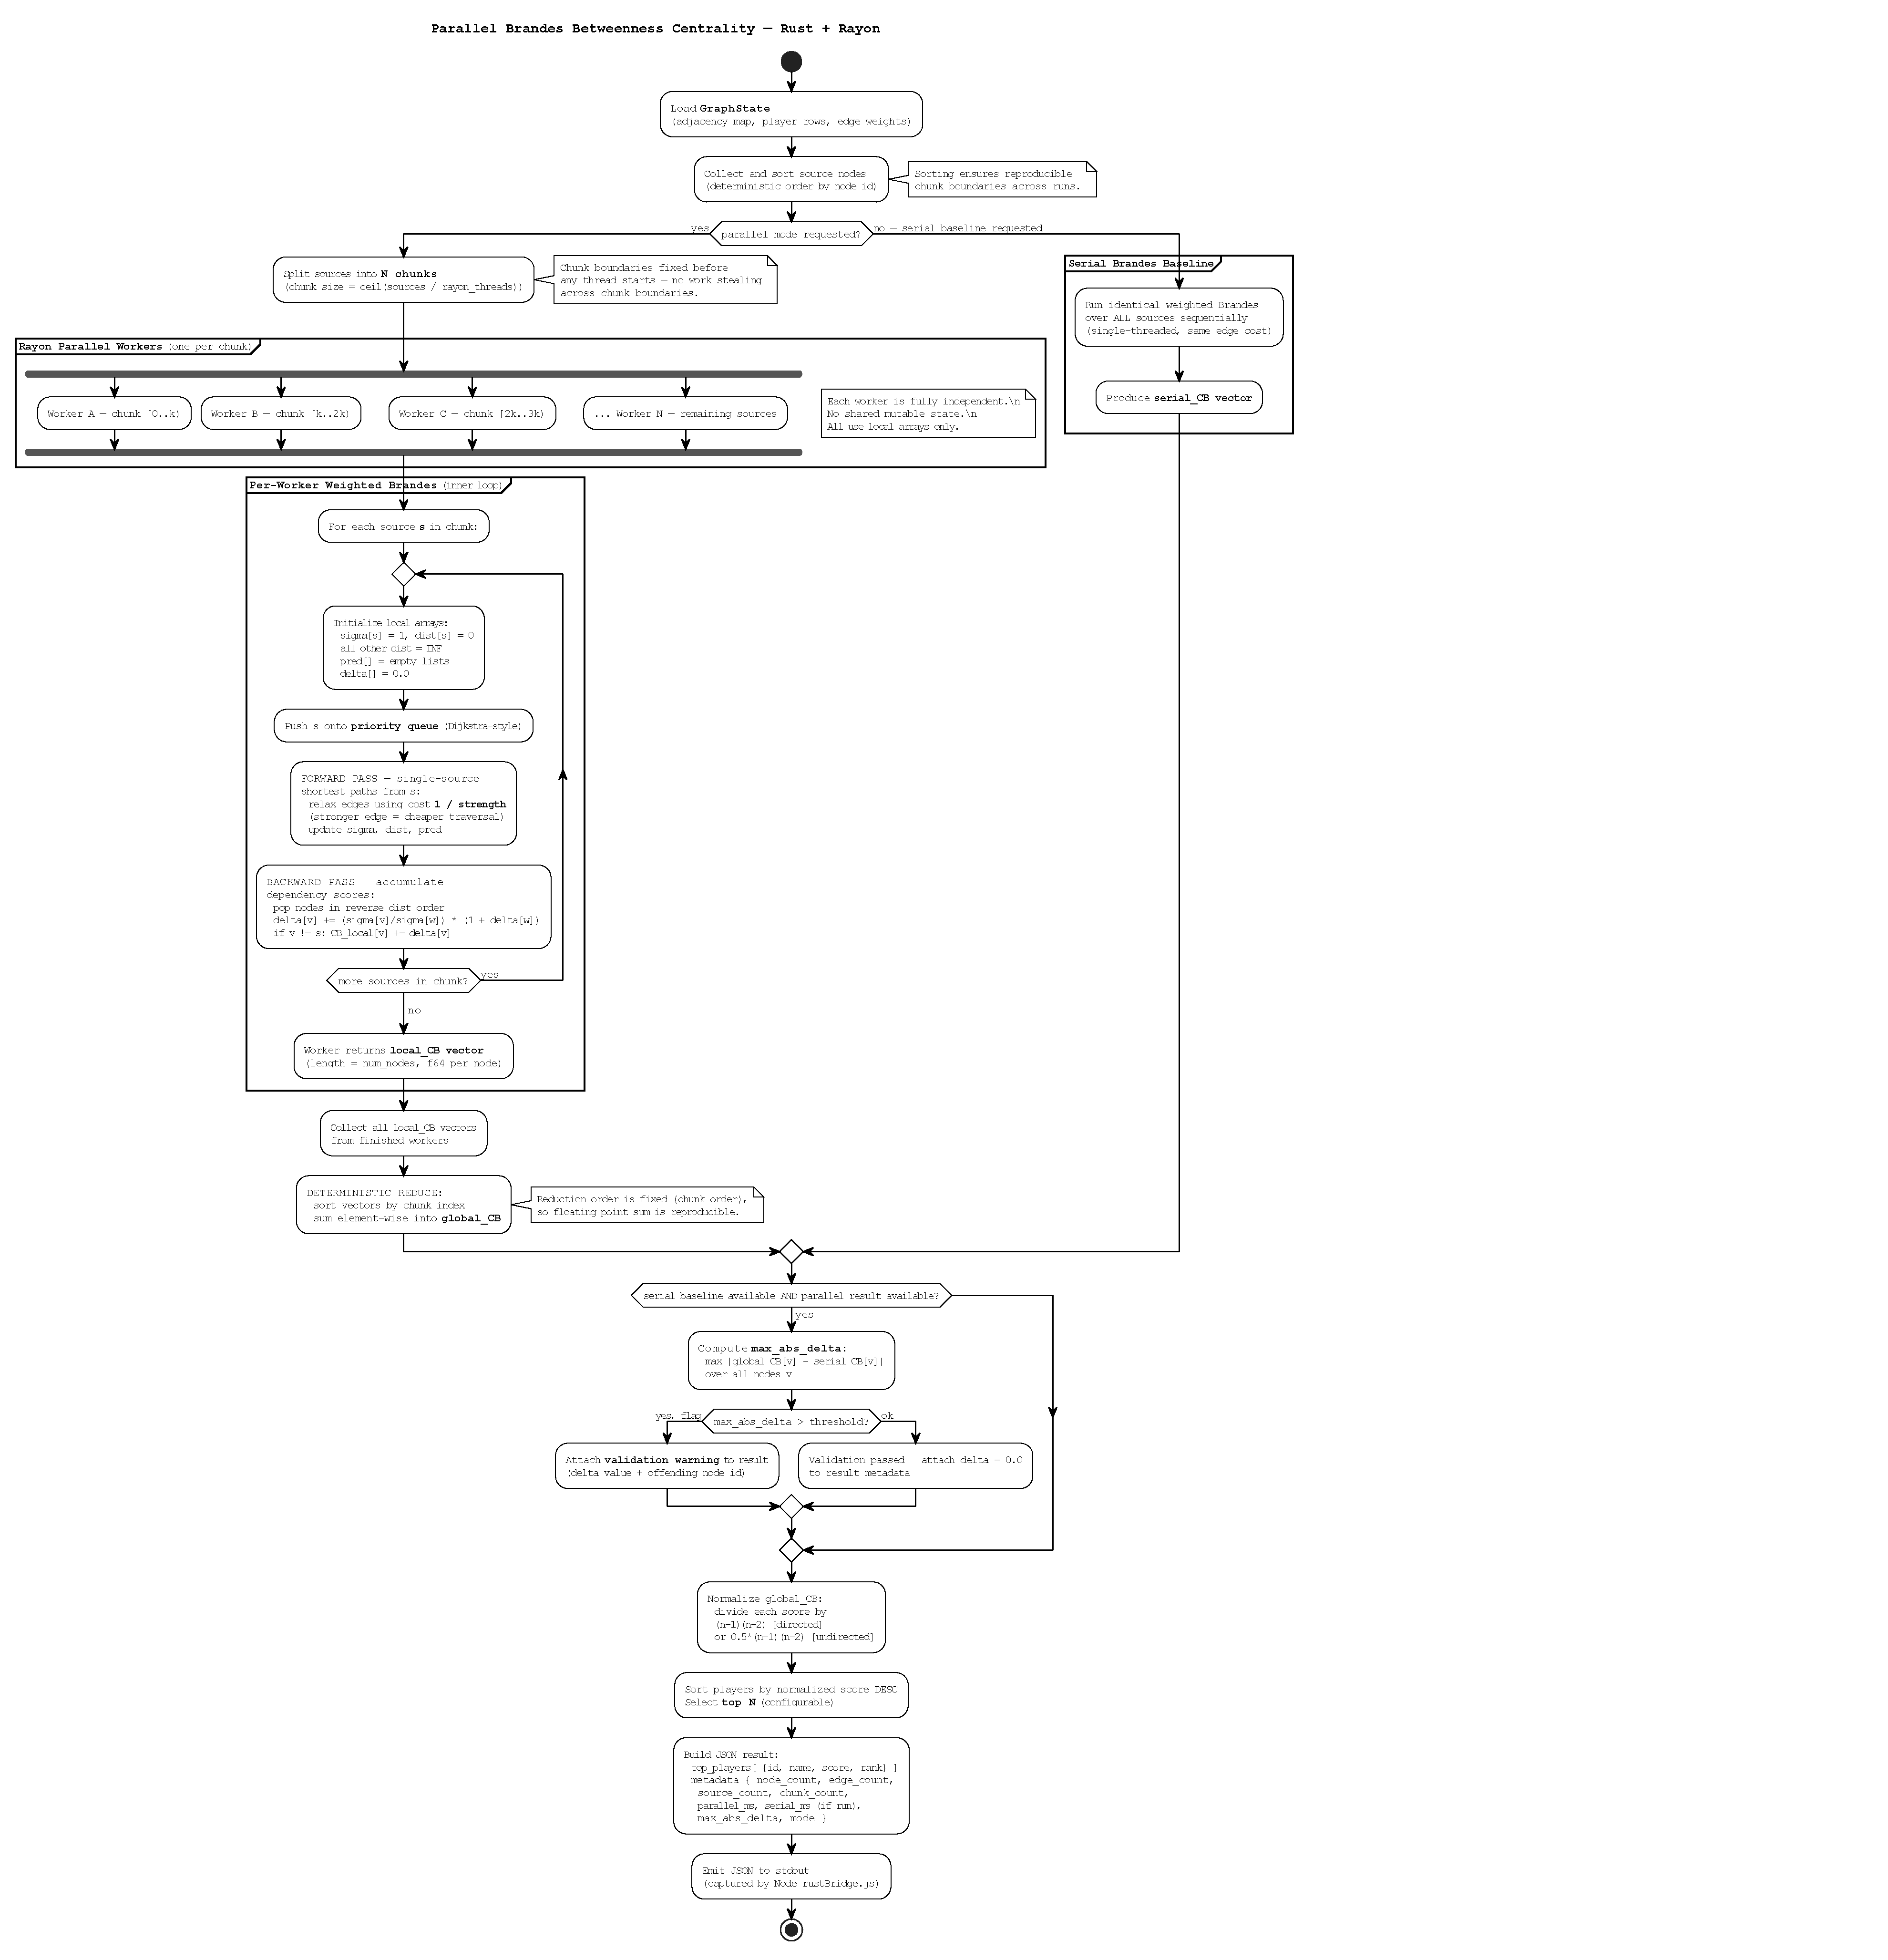
\includegraphics[width=\textwidth,height=0.88\textheight,keepaspectratio]{parallel brandes activity diagram.pdf}
\label{fig:parallel-brandes-activity}
\caption{A párhuzamos Brandes-futtatás aktivitásdiagramja a \texttt{parallel-brandes.puml} forrás alapján. A folyamat a \texttt{GraphState} betöltésével és a forráscsomópontok determinisztikus rendezésével indul, majd párhuzamos módban fix chunkokra bontja a forrásokat. Minden Rayon worker saját lokális tömbökkel futtat súlyozott Brandes-bejárást, \texttt{1/strength} élköltséggel; a lokális centralitásvektorok chunk-sorrendben, determinisztikusan redukálódnak globális eredménnyé. Ha soros baseline is készül, a rendszer \texttt{max\_abs\_delta} értékkel ellenőrzi a párhuzamos és soros kimenet egyezését, majd normalizál, rangsorol és JSON választ ad vissza a Node.js hídnak.}
\end{figure}

\begin{figure}[H]
\centering
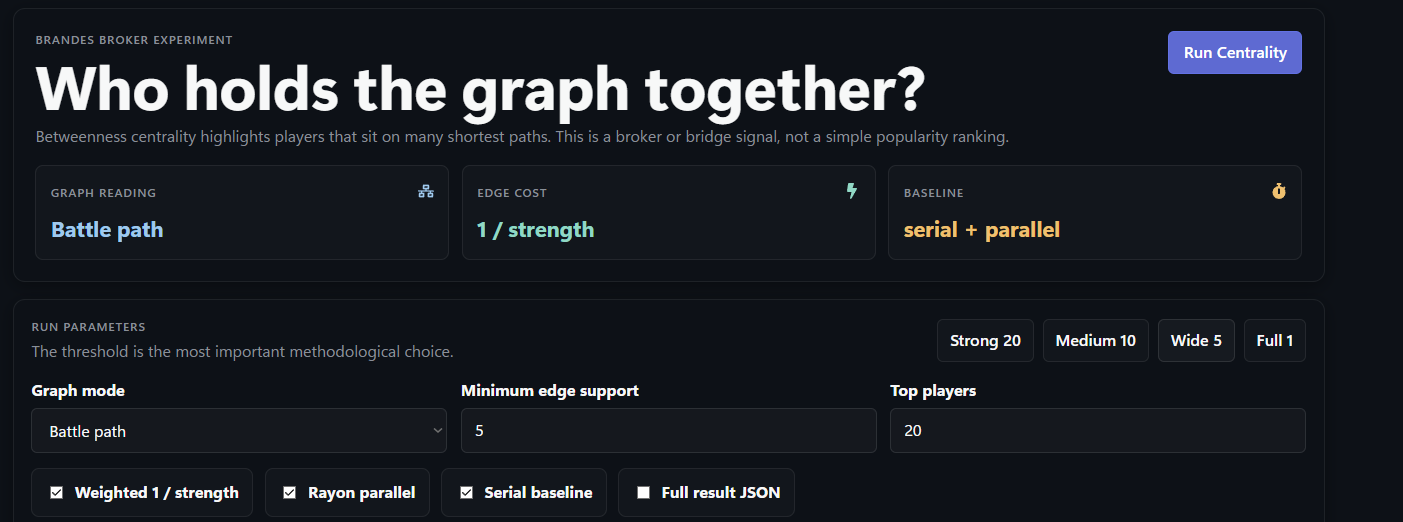
\includegraphics[width=0.98\textwidth,height=0.52\textheight,keepaspectratio]{brandes-config.png}
\caption{A Brandes betweenness centralitás frontend konfigurációs felülete. A képen a \textit{battle-path} gráfolvasat, az $1/\text{strength}$ élköltség, a soros és párhuzamos baseline összehasonlítás, az 5-ös minimum éltámogatás, a top 20 játékos kérése, valamint a súlyozott, Rayon-párhuzamos és soros baseline opciók láthatók.}
\end{figure}

\begin{table}[H]
\centering
\caption{A betweenness centralitás-modul főbb konfigurációs dimenzióinak összefoglalója}
\begin{tabular}{lll}
\toprule
\textbf{Dimenzió} & \textbf{Lehetséges értékek} & \textbf{Hatás} \\
\midrule
Gráfmód & social-path, battle-path & Melyik élhalmazon fut \\
Súlyozás & igen / nem & Élköltség kiszámítása \\
Párhuzamos & igen / nem & rayon vs. soros Brandes \\
Soros baseline & igen / nem & Delta-ellenőrzés a kimenetben \\
Min. élsúly & $\geq 1$ & Gyenge élek kizárása \\
\bottomrule
\end{tabular}
\end{table}

\subsection{Projekció és normalizálás}

A \textit{build\_projection()} a \textit{GraphState} pair\_relations térképéből iterál; az élek sorrend szerint rendezve kerülnek feldolgozásra, így a projekció determinisztikus. Kizárásra kerülnek a nulla support értékű élek, a minimum élsúly alattiak és a rossz formátumú kulcsú élek. A csomópontok ábécé-sorrendben indexelődnek, és a szomszédsági lista minden csúcsnál szintén rendezett, ami garantálja a determinizmust akkor is, ha a belső tárolás bejárási sorrendje változó.

A normalizált betweenness érték $[0, 1]$ intervallumba esik, ahol az 1.0 értékű csomópont minden lehetséges legrövidebb úton rajta van. Az egységtesztek lánc-, csillag- és dumbbell-topológián, súlyozási eseteken és soros-párhuzamos egyezésen ellenőrzik a helyes viselkedést.

\begin{figure}[H]
\centering
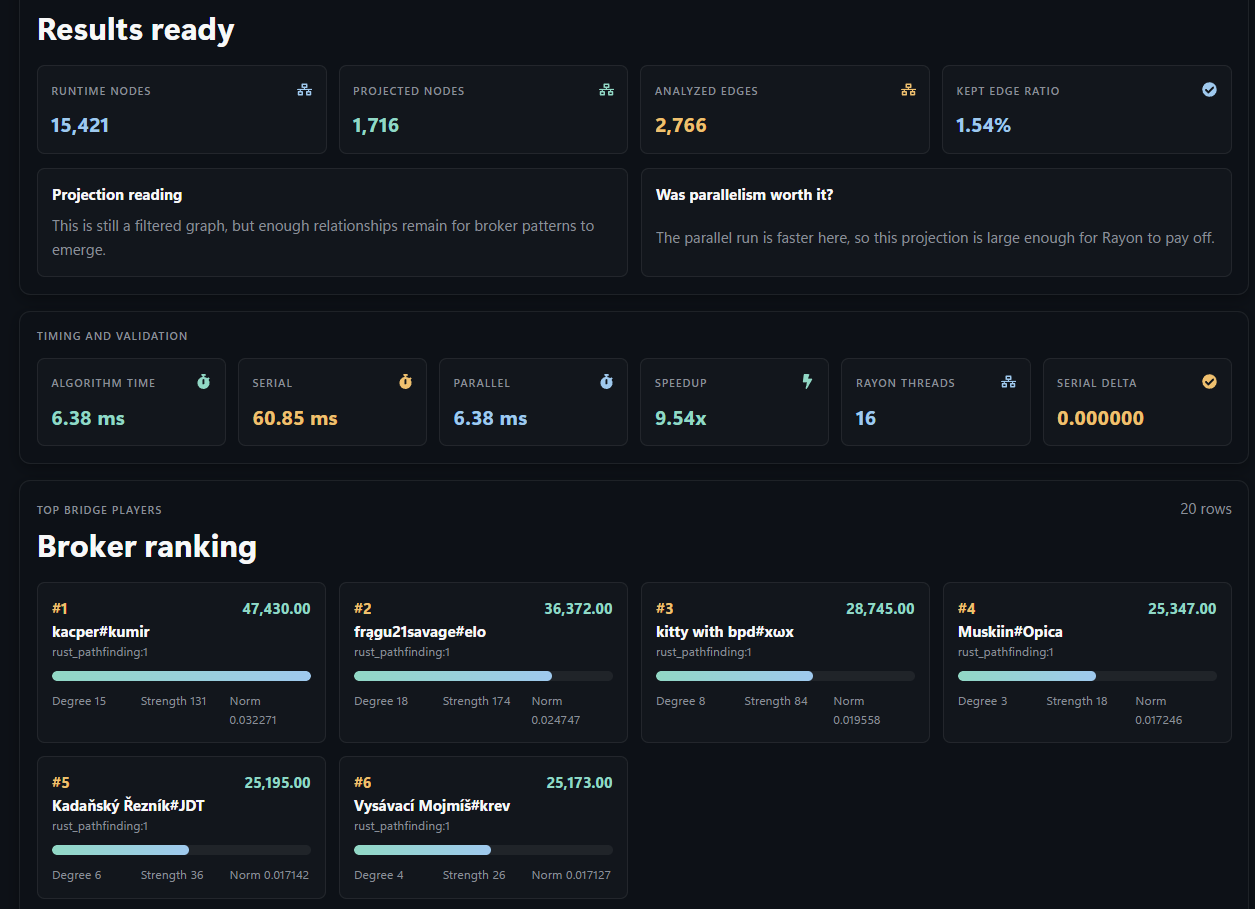
\includegraphics[width=0.98\textwidth,height=0.68\textheight,keepaspectratio]{brandes-result.png}
\caption{Brandes betweenness centralitás eredményképernyő. A futás 15\,421 runtime csomópontból 1\,716 projektált csomópontot és 2\,766 elemzett élt tartott meg (1.54\%-os megtartott élhányad). A párhuzamos futás 6.38 ms alatt, a soros baseline 60.85 ms alatt futott, 9.54-szeres gyorsulással, 16 Rayon szállal és 0.000000 soros-párhuzamos deltával; alul a top broker játékosok rangsora látható raw és normalizált centralitási értékekkel.}
\end{figure}

\begin{figure}[H]
\centering
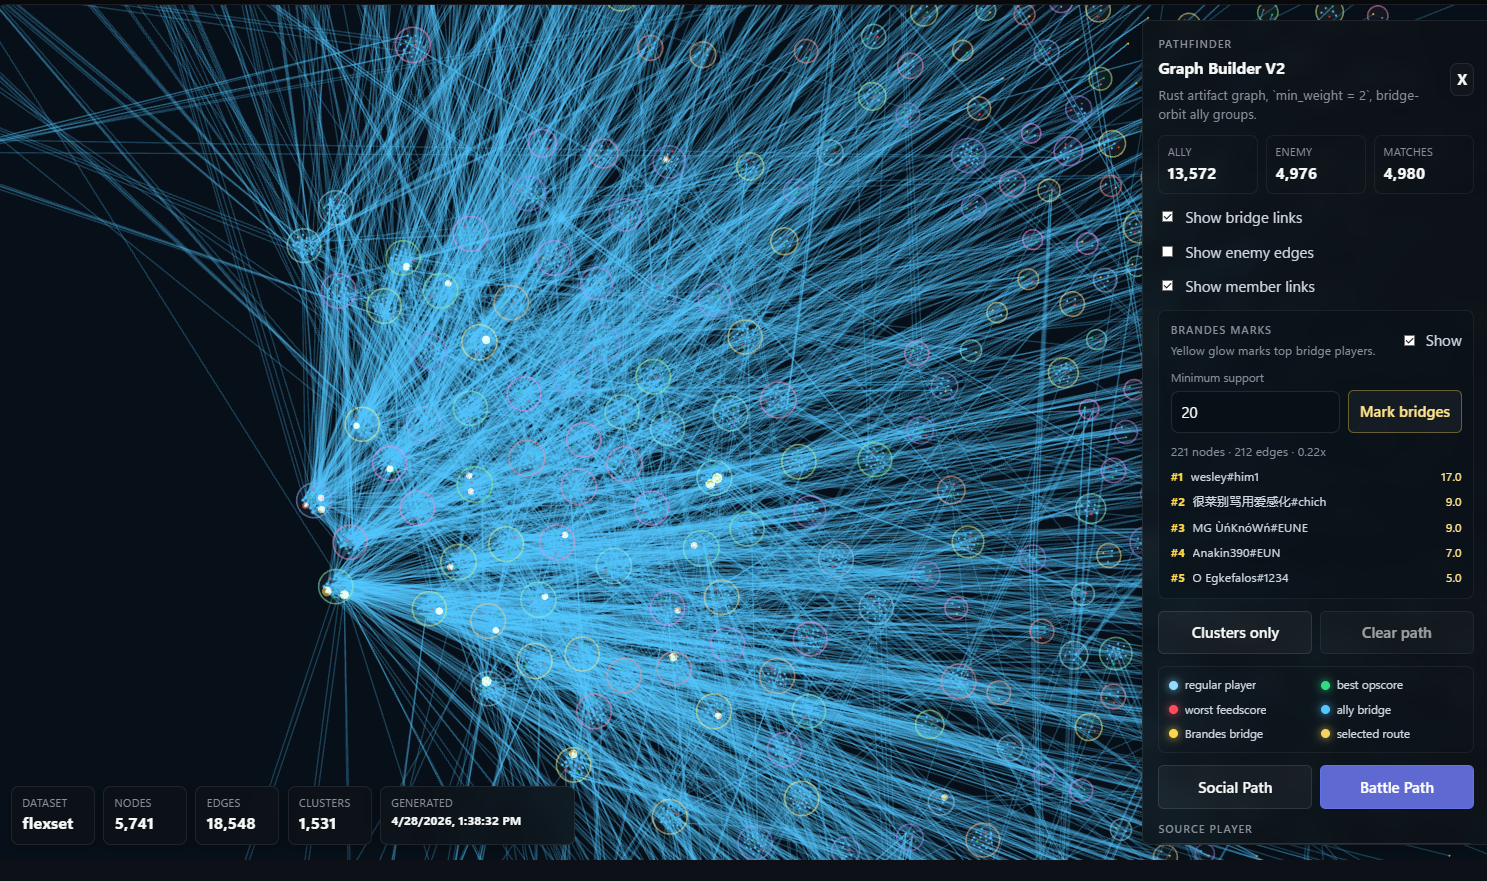
\includegraphics[width=\textwidth,height=0.78\textheight,keepaspectratio]{graph-brandes-brokerinyellow.png}
\caption{A betweenness centralitás alapján azonosított broker játékosok a gráfban, sárgával kiemelve. A kiemelés azokat a csomópontokat jelöli, amelyek normalizált betweenness értéke a legmagasabb; ezek a bridge-jelöltek az \textit{orbitScore}-alapú vizuális heurisztika és a tényleges topológiai centralitás összevetésének kiindulópontja.}
\end{figure}

A legmagasabb \textit{crossAllySupport} és \textit{connectedAllyClusterCount} értékű klaszterek átlagos Brandes-betweenness értékének összevetése az alacsony orbit-score-úakéval elvégezhető a modul segítségével: ha a hipotézis teljesül, az megerősíti, hogy az orbit-heurisztika jó előszűrője a valódi topológiai hidat képező csomópontoknak.

\section{Kísérletfuttató infrastruktúra}

A Rust motor az egyedi analitikai kérések mellett strukturált kísérleteket is tud futtatni az \textit{engine/experiments.rs} modulon keresztül.

A signed-balance sweep (\textit{SignedBalanceSweepRequest}) egyszerre több minimum-élsúly és döntetlen-kezelési politika kombinációt futtat le, és az összes eredményt egyetlen válaszban adja vissza. A dolgozatban ezt már nem fő eredményként, hanem annak ellenőrzésére használjuk, hogy mennyire erősen függ a formális signed-balance kimenet a projekciós döntésektől; a sweep a módszertani határ dokumentálására szolgál.

Az asszortativitási szignifikanciateszt (\textit{AssortativitySignificanceRequest}) permutációs nullmodellt futtat: véletlenszerűen kever össze játékos--score párokat az éleken, és az így kapott null-eloszlással veti össze a megfigyelt korrelációt. A permutáció-szám konfigurálható, a determinisztikus RNG-mag garantálja a reprodukálhatóságot. A jelen dolgozatban a szignifikanciafuttatások léte dokumentált, de az összes kombinációra kiterjedő, végleges nullmodell-kísérletsorozat a jövőbeli fejlesztések közé tartozik.

\section{Validáció és rendszerkoherencia}

A dolgozat elkészítésekor a rendszer aktuális állapota közvetlen futtatás alapján is ellenőrzésre került: a Rust futtatókörnyezet sikeresen lefuttatta az \textit{assortativity} és \textit{betweenness-centrality} parancsokat, a dataset-regiszter olvasható volt, a frontend analitikai útvonalak fizikailag jelen voltak. A verifikáció nem teljes funkcionalitásteszt, hanem tézisszintű ellenőrzés: minden olyan rétegről legyen közvetlen bizonyíték, amelyre a dolgozat állításokat épít \cite{sandve2013}.

A \ref{fig:validation-pipeline}. ábra a dolgozati bizonyítékok teljes validációs pipeline-ját mutatja be, a dataset-regisztertől a PDF-fordításig.

\begin{figure}[H]
\centering
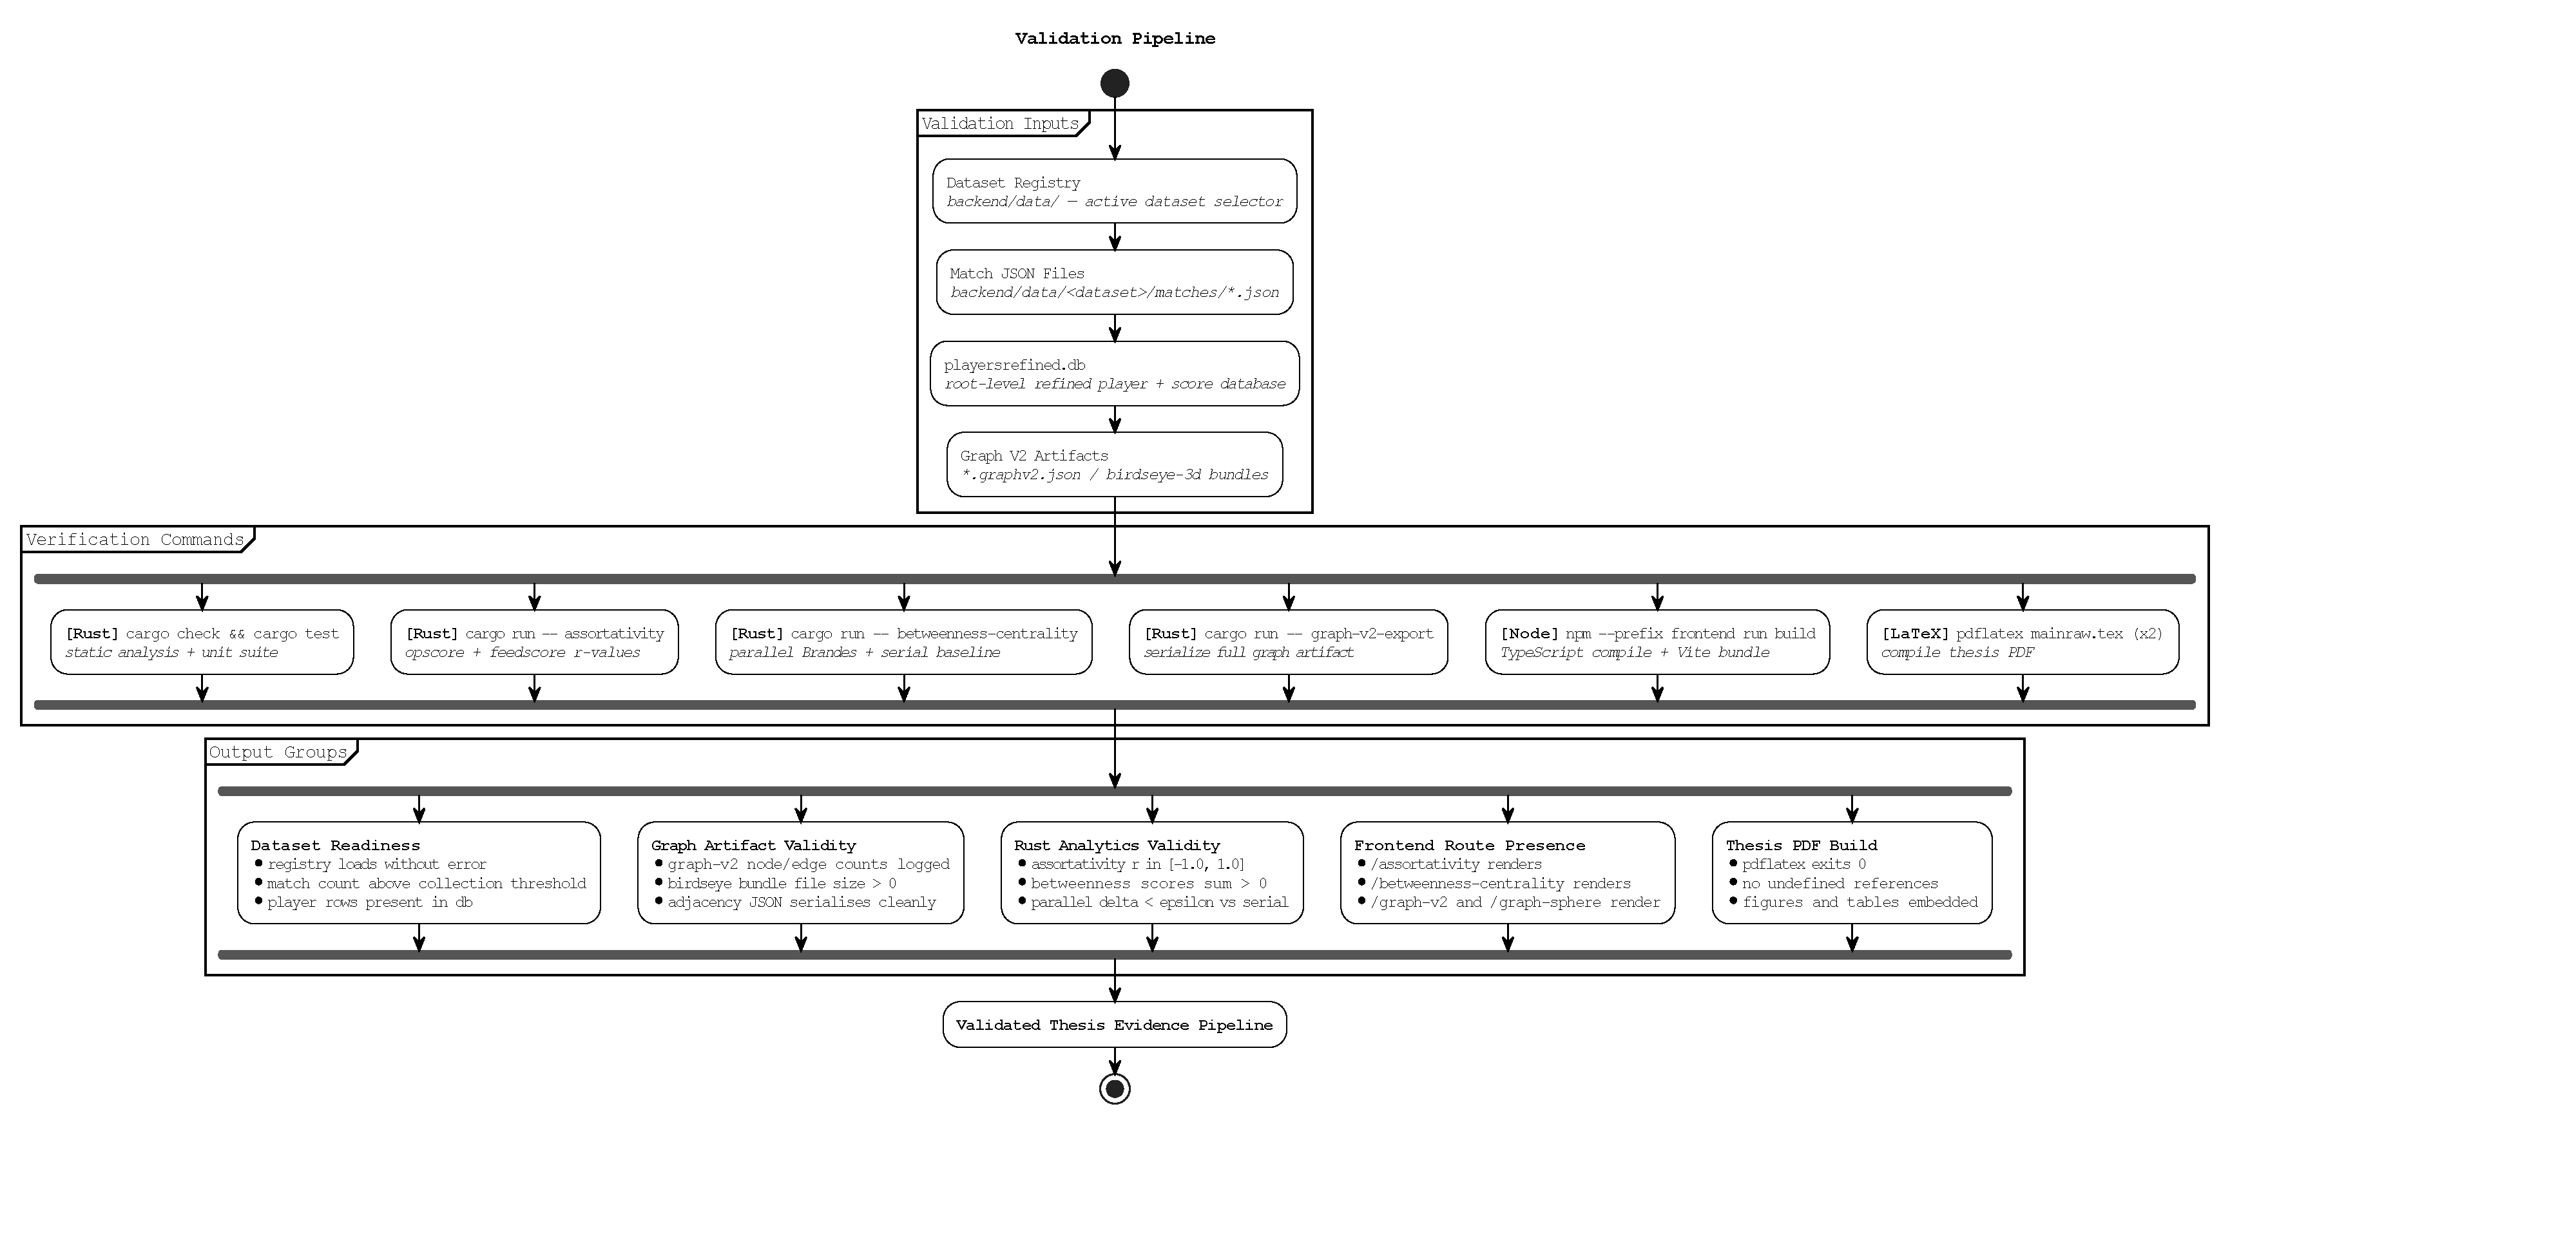
\includegraphics[width=\textwidth,height=0.88\textheight,keepaspectratio]{validation_pipeline.pdf}
\label{fig:validation-pipeline}
\caption{A dolgozati bizonyítékok validációs pipeline-ja a \texttt{thesis-validation-pipeline.puml} forrás alapján. A diagram először a validációs bemeneteket mutatja: dataset-regiszter, meccs-JSON állományok, \texttt{playersrefined.db} és Graph V2 artifactok. Ezután párhuzamos ellenőrzési parancsokra bontja a folyamatot: Rust \texttt{cargo check}/\texttt{cargo test}, asszortativitás, Brandes-betweenness, Graph V2 export, frontend build és dolgozati PDF-fordítás. A kimeneti csoportok külön ellenőrzik a dataset-készültséget, a gráfartifactok érvényességét, a Rust analitikák tartomány- és deltafeltételeit, a frontend útvonalak jelenlétét és a PDF build sikerét.}
\end{figure}

A projekt egyik fontos eredménye az is, hogy a rendszer ma már koherens egészként működik. Az adatgyűjtés és dataset-kezelés külön rétegben történik; a pontszámítás explicit, ellenőrizhető képletekre épül; a gráfépítés és klaszterezés nem ad hoc frontend-logika; a futásidejű Rust réteg a gráfanalitikát külön kezeli; a frontend több specializált felületen, eltérő célok mentén mutatja meg az eredményeket. A Signed Balance route a dolgozati termékből kikerült, mert a fő narratíva már nem erre az értelmezésre épül.

% Ez a fejezet összevonásra került a 16-os fejezettel (Gráfanalitikai eredmények: asszortativitás és betweenness centralitás).

\chapter{Kísérleti futtatások, validáció és eredmények}

\section{Verifikációs lépések}

A dolgozat elkészítésekor a rendszer aktuális állapotát nemcsak a dokumentáció, hanem közvetlen futtatás alapján is ellenőriztem. A főbb helyi ellenőrzések:

\begin{itemize}
    \item a Rust futtatókörnyezet sikeresen lefuttatta az \texttt{assortativity} parancsot;
    \item a Rust futtatókörnyezetben a \texttt{signed-balance} parancs kísérleti modulként továbbra is futtatható volt;
    \item a fő adatbázis és dataset-nyilvántartás elérhető és olvasható volt;
    \item a dolgozati frontend útvonalak közül az asszortativitási és központisági oldalak maradtak a fő analitikai folyamat részei.
\end{itemize}

Ez azért lényeges, mert a dolgozat ezen a ponton már nem csak tervekről, hanem ténylegesen végrehajtható modulokról számol be.

A verifikációs lépések tudatosan nem teljes funkcionalitástesztek voltak, hanem tézisszintű ellenőrzések. A cél itt az volt, hogy minden olyan rétegről legyen közvetlen bizonyíték, amelyre a dolgozat állításokat épít: a dataset-regiszter olvashatósága, a Rust analitikai parancsok futtathatósága, valamint a frontendoldalak fizikai jelenléte. Ez összhangban van a reprodukálható kutatási gyakorlat logikájával is: a szöveg és az alátámasztó futások között legyen világos kapcsolat \cite{sandve2013}.

\section{Az aktív állapot összefoglalása}

A 2026. április 28-án ellenőrzött aktív állapotban a rendszer az \texttt{soloq} datasetre épül, a \texttt{flexset} dataset a fő kutatási korpusz. Az adatkészletek és a gráfállapot összefoglalása:

\begin{table}[H]
\centering
\caption{A jelenlegi rendszerállapot fő mennyiségi mutatói - \texttt{flexset} és \texttt{soloq}}
\begin{tabular}{lrr}
\toprule
\textbf{Mutató} & \textbf{flexset} & \textbf{soloq} \\
\midrule
Meccs-JSON állományok & 4981 & 2001 \\
Graph V2 meccsszám & 4980 & 2000 \\
Nyers játékosok (\texttt{players.db}) & 15\,147 & 2822 \\
Finomított játékosok (\texttt{playersrefined.db}) & 15\,421 & 6768 \\
Klaszterek (\texttt{playersrefined.db}) & 599 & 140 \\
Klasztertagok & 5741 & 1538 \\
Látható Graph V2 csúcsok & 5741 & 1538 \\
Látható Graph V2 élek & 18\,548 & 4111 \\
Átlagos élsúly (Graph V2) & 3.405 & 2.364 \\
Graph V2 klaszterek & 1531 & 870 \\
Átlagos klaszterméret & 3.750 & 1.768 \\
\bottomrule
\end{tabular}
\end{table}

Ezeket a számokat lépcsőzetesen kell olvasni. A finomított játékosszám a teljes score-réteg kiterjedése. A Graph V2 látható csúcsok száma már csak az érvényes klasztertagsággal rendelkező játékosokat tartalmazza. Minden réteg a saját, a megelőzőből leszűkített univerzumán számol, ezért a gráf- és score-alapú eredményeknél mindig ki kell mondani, hogy pontosan melyik populáción készültek.

A két dataset összehasonlítása megerősíti, hogy a \texttt{flexset} és a \texttt{soloq} lényegesen eltérő karakterű korpuszok, és ez az eltérés minden analitikai szinten mérhető.

\section{A korpusz összetétele mint értelmezési háttér}

Az eredmények értékeléséhez fontos hozzárakni, hogy a vizsgált korpusz nem homogén. A queue-eloszlás alapján a ranked módok dominálnak, de a rendszerben ARAM és normál meccsek is jelen vannak. Ez két következménnyel jár:

\begin{itemize}
    \item a gráf egy része erősen kompetitív, ismétlődő társas térből származik;
    \item egy másik része lazább, zajosabb kapcsolatokkal terhelt.
\end{itemize}

Éppen ezért a küszöbölés, az erős és gyenge kapcsolatok bontása, valamint a \texttt{social-path} és \texttt{battle-path} megkülönböztetése nem puszta technikai részlet, hanem az adatkorpuszból fakadó szükségszerűség.

Ez a felismerés a teljes eredményfejezetet meghatározza. Ha a korpusz heterogén, akkor a gráfmodellt sem lehet úgy kezelni, mintha egyetlen társas mechanizmust mérne. A \texttt{social-path} és \texttt{battle-path} különválasztása nem csupán algoritmus-beállítás, hanem módszertani védekezés a túlzó interpretáció ellen.

\section{A két klasztercsalád gyakorlati különbsége}

A perzisztált klasztereknél az is ellenőrizhető volt, hogy a Python és a Rust család eltérő karakterű. A \texttt{python\_population} klaszterek kicsit kisebb maximális méretűek és inkább populációs közösségképet adnak, míg a \texttt{rust\_pathfinding} klaszterek futásidejű szempontokhoz igazodnak, és jóval nagyobb maximumklasztert is tartalmaznak.

Ez összhangban van a rendszertervvel. A két klasztercsalád nem egymás hibás duplikátuma, hanem eltérő feladatokra optimalizált nézet.

\section{Analitikai eredmények}

Az asszortativitási eredmények részletes táblái és módszertani kifejtése a dedikált fejezetben kapott helyet. A strukturális egyensúly külön fejezetben csak módszertani határesetként szerepel: a formális implementáció megvan, de az enemy-élek szemantikája miatt nem használom fő empirikus eredményként. A két dataset összesített, szintetikus összehasonlítása a rákövetkező összehasonlító fejezetben található.

\section{A frontend és a rendszerkoherencia értékelése}

A projekt egyik fontos eredménye nem kizárólag a számszerű analitikában áll, hanem abban is, hogy a rendszer ma már koherens egészként működik. A jelenlegi állapotban:

\begin{itemize}
    \item az adatgyűjtés és dataset-kezelés külön rétegben történik;
    \item a pontszámítás explicit, ellenőrizhető képletekre épül;
    \item a gráfépítés és klaszterezés nem ad hoc frontend-logika;
    \item a futásidejű Rust réteg a gráfanalitikát külön kezeli;
    \item a frontend több specializált felületen, eltérő célok mentén mutatja meg az eredményeket.
\end{itemize}

Ez azért fontos, mert a dolgozat nem egyszerűen egy algoritmus vagy egy látványos oldal bemutatása, hanem annak dokumentálása, hogy ezek a részek együtt már egy kutatásképes rendszerként viselkednek.

A koherencia egyik kézzelfogható jele, hogy a frontend route-struktúrája és a backend végpontstruktúrája egymásra illeszkedik. A \texttt{frontend/src/App.tsx} külön oldalakat tart fenn a collectorhoz, a graph sphere-höz, az assortativity-hez, a betweenness-központisághoz és a Pathfinder Labhoz, vagyis a felület nem egyetlen „mindent bele” dashboard. A Signed Balance route a dolgozati termékből kikerült, mert a fő narratíva már nem erre az értelmezésre épül.

\section{A korábbi ország-elemzési ág helye a jelenlegi rendszerben}

A korábbi \texttt{assign\_countries.py} és \texttt{conclude.py} ág továbbra is a projekt része. Ez megőrzi azt a lehetőséget, hogy a klaszterekből származó országcímkézést összekapcsoljuk aggregált teljesítményelemzéssel. Ugyanakkor a jelenlegi dolgozat fő tudományos súlypontja már nem ez, hanem a gráf mint kutatási objektum.

Védhetőnek azt tartom, ha ezt az ország-elemzési vonalat \emph{kiegészítő, exploratív} modulnak nevezzük:

\begin{itemize}
    \item implementált,
    \item hasznos lehet,
    \item de bizonytalansága nagyobb,
    \item ezért a dolgozat központi állításait nem erre építem.
\end{itemize}

\begin{figure}[H]
\centering
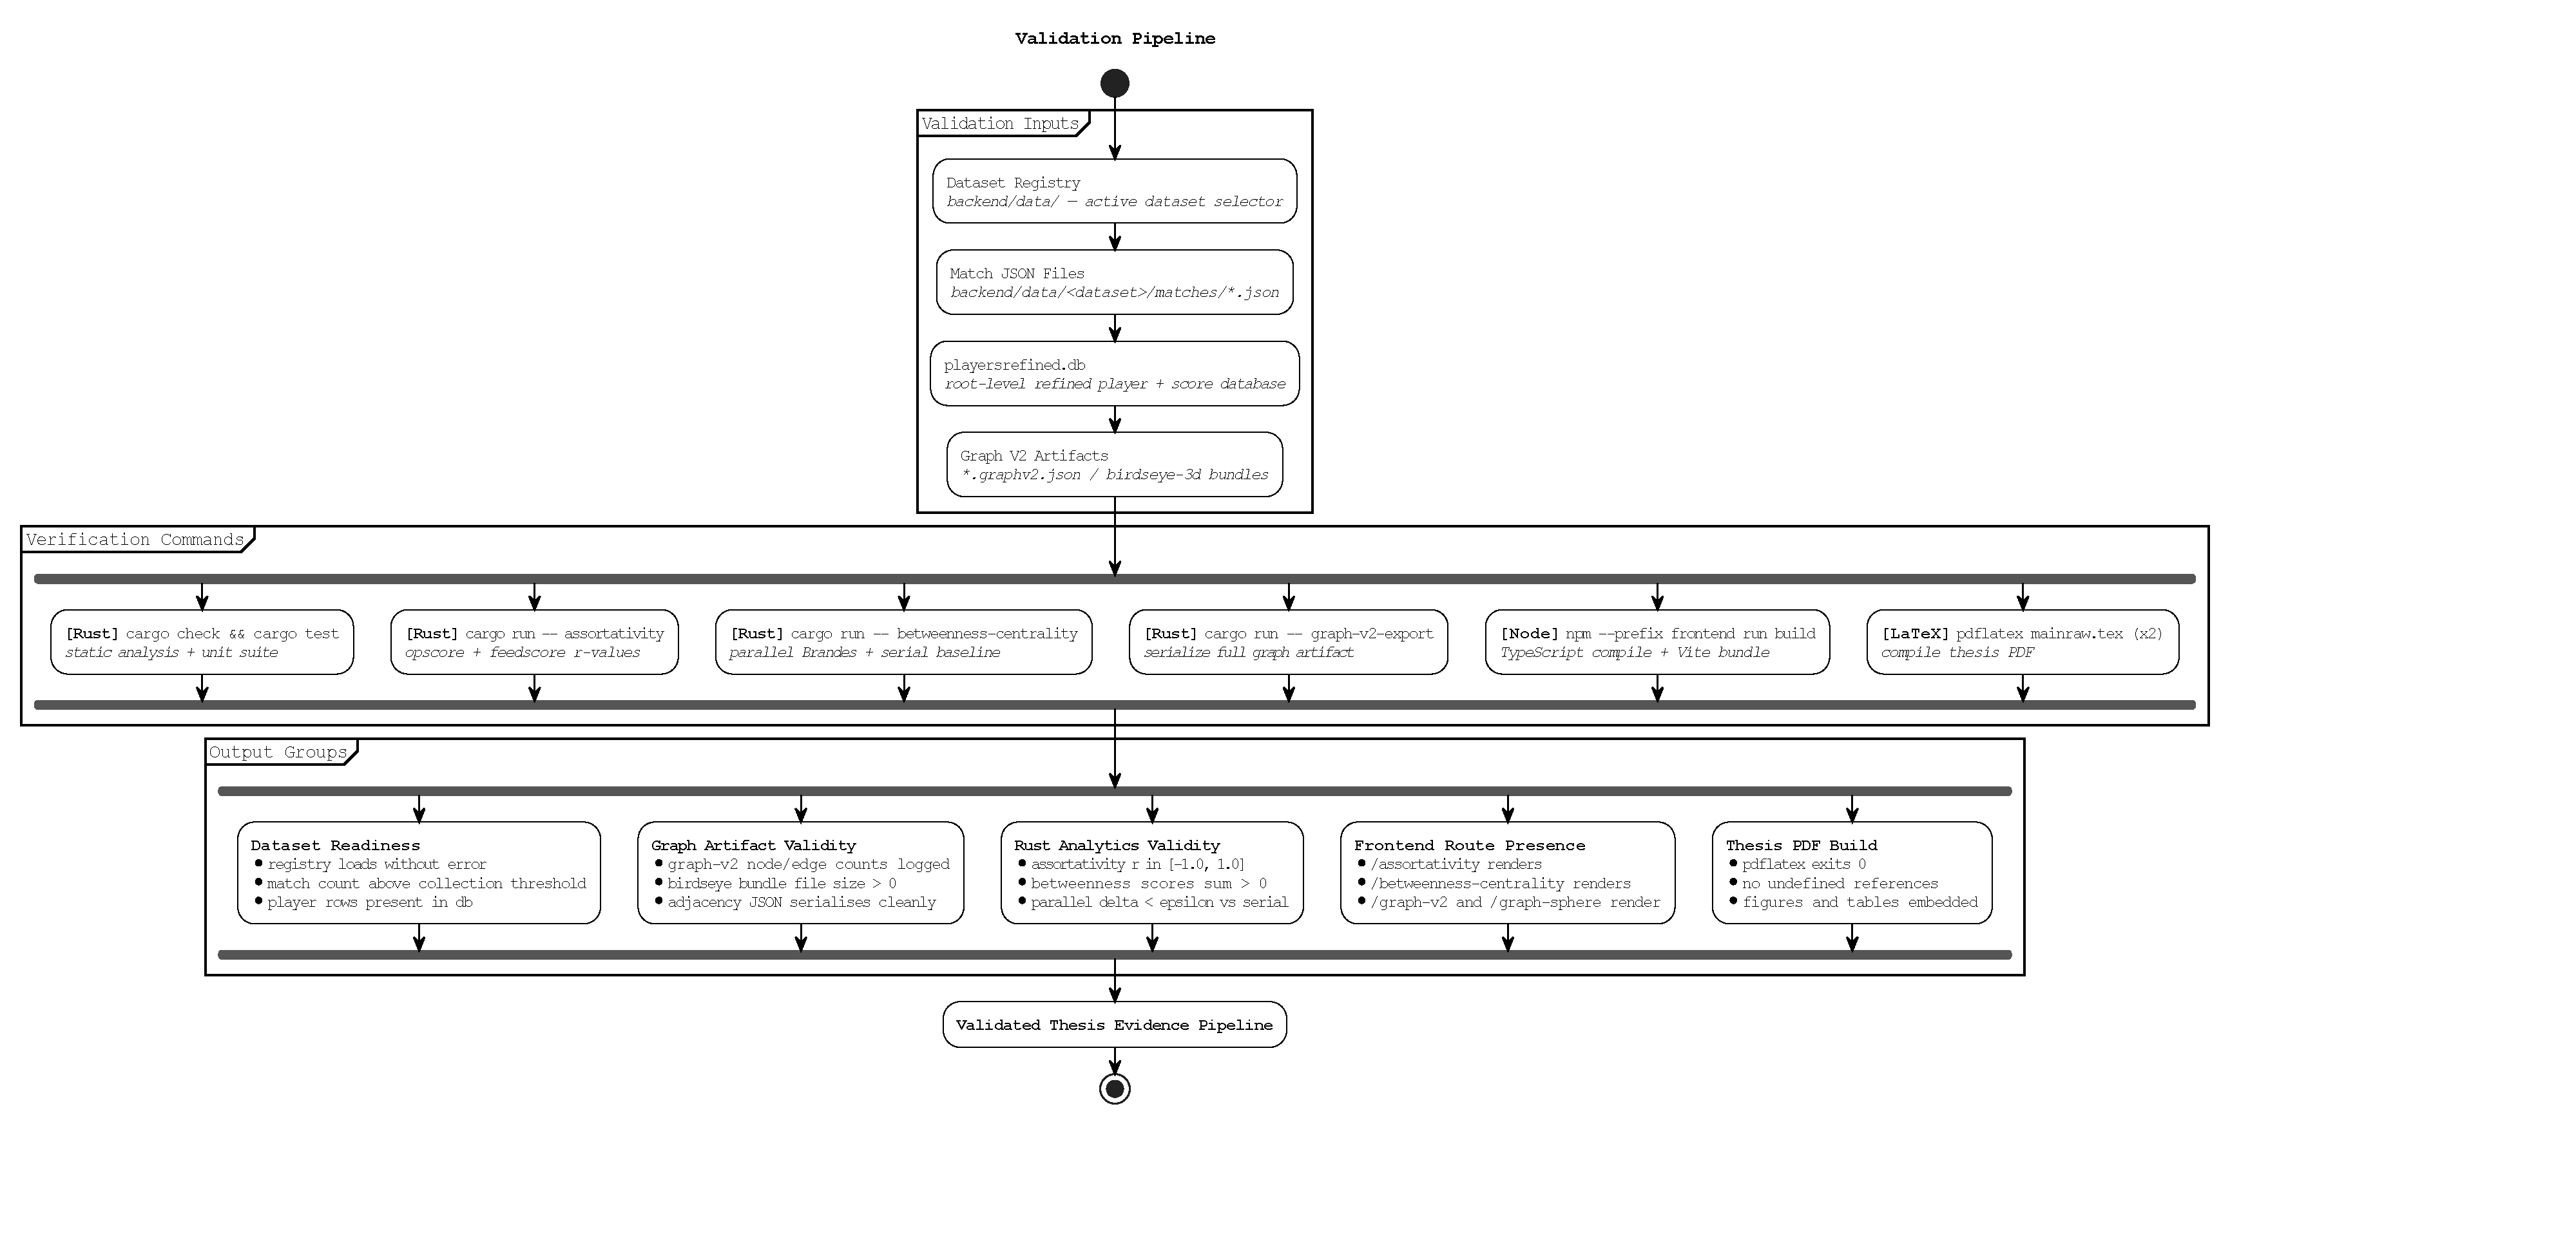
\includegraphics[width=0.98\textwidth,height=0.76\textheight,keepaspectratio]{validation_pipeline.pdf}
\caption{A dolgozati bizonyítékok validációs pipeline-ja a \texttt{thesis-validation-pipeline.puml} forrás alapján. A diagram először a validációs bemeneteket mutatja: dataset-regiszter, meccs-JSON állományok, \texttt{playersrefined.db} és Graph V2 artifactok. Ezután párhuzamos ellenőrzési parancsokra bontja a folyamatot: Rust \texttt{cargo check}/\texttt{cargo test}, asszortativitás, Brandes-betweenness, Graph V2 export, frontend build és dolgozati PDF-fordítás. A kimeneti csoportok külön ellenőrzik a dataset-készültséget, a gráfartifactok érvényességét, a Rust analitikák tartomány- és deltafeltételeit, a frontend útvonalak jelenlétét és a PDF build sikerét.}
\end{figure}

\chapter{Rendszerszintű értékelés és megvitatás}

\section{A legfontosabb rendszertervezési döntések}

Az egész projektet visszanézve a legerősebb döntésnek az tekinthető, hogy a különböző feladatok nem kerültek egyetlen univerzális technológiába kényszerítve. A rendszer nem eszközpreferencia, hanem minőségi attribútumok mentén fejlődött: reprodukálhatóság, magyarázhatóság, perzisztencia, futási teljesítmény és demo-koherencia. Ezeket ritkán lehet mindent ugyanazzal az eszközzel a legjobban kiszolgálni.

A Python gyors iterációt és kényelmes adatfeldolgozást ad, a Rust teljesítményt és pontos gráfkontrollt, a Node/Express stabil integrációs felületet, a React pedig erős bemutathatóságot. A többnyelvűség tehát nem öncélú komplexitás, hanem funkcionális specializáció.

\section{A rendszer erősségei}

A projekt legfontosabb erőssége, hogy a teljes adatút végigkövethető a Riot API-tól a frontendig: nincsenek kézzel összeollózott közbenső lépések. A játékosprofilok explicit, ellenőrizhető képleteken és mezőkön alapulnak; a gráfépítés és klaszterezés nem csak vizuális export, hanem perzisztens objektum, amelynek bejárása és újraelőállítása determinisztikus. A Rust réteg valódi analitikai és futtatási értéket ad, nem csupán egy korábbi Python-szkript gyorsabb átírása. Az asszortativitás, a core-periphery gráfolvasat és a Brandes-centralitás valódi kutatási kérdésekké emelik a rendszert, amelyeket az implementáció közvetlenül tud megválaszolni.

\section{Érvényességi fenyegetések}

A projekt legfontosabb validitási kockázata, hogy a dataset nem reprezentálja a teljes játékospopulációt: a gyűjtés seed- és queue-függő, ezért a mintavétel nem véletlen. Az \textit{opscore} és \textit{feedscore} értelmezhető, de nem objektív igazságmérő: különösen az \textit{opscore} tartalmaz kézi szerepkör-súlyozást. A retired signed-balance ág nem kap fő empirikus szerepet, mert az enemy-él negatív társas kötésként való értelmezése nem elég erős. Az ország-elemzési ág sokkal bizonytalanabb, mint a közvetlen gráf- és meccsanalitika, és ezért nem képezi a főeredmények részét.

Rétegenként szétbontva: a \textbf{mintavételi validitás} szempontjából a seedválasztás, a premade-probe és a queue-orientáció együtt nem véletlen mintát adnak a teljes játékospopulációból. A \textbf{mérési validitás} szempontjából az \textit{opscore} és \textit{feedscore} értelmezhetők, de konstrukciós döntésekre épülnek. A \textbf{projekciós validitás} szempontjából a gráfmód, az élküszöb és az ally/enemy kapcsolatértelmezés érdemben alakítja a végső analitikai mintát: a signed-balance emiatt csak módszertani határesetként kezelhető. A \textbf{klasztervaliditás} szempontjából a közösségdetektálás eredménye függ a választott gráftól, a küszöböléstől és a modularitás felbontási korlátjától \cite{fortunato_barthelemy2007}. A \textbf{temporális validitás} szempontjából a korpusz fokozatosan épülő archívum, ezért a teljes háló nem egyetlen szinkron időpillanat felvétele.

Ezek a fenyegetések nem rombolják le a dolgozatot. Inkább kijelölik azt a határt, amelyen belül az állítások védhetők, és a bírálat szempontjából sokkal erősebb pozíciót ad egy rétegzetten dokumentált korlát, mint egy rejtett módszertani gyengeség.

\section{A megvalósult és a jövőbeli elemek szétválasztása}

A dolgozat egyik tudatos módszertani döntése az volt, hogy a jelenleg implementált és a még csak tervezett elemeket nem keveri össze. A ténylegesen megvalósult mag a Riot API-ra épülő adatgyűjtésből, \textit{puuid}-alapú normalizálásból, \textit{feedscore}/\textit{opscore} számításból, legacy Python exportból és populációs közösségdetektálásból, SQLite klaszterperzisztenciából, Rust Graph V2 gráfépítésből, útvonalkeresésből, asszortativitásból, Brandes-centralitásból és 3D globális exportból áll. Ehhez adódik a databaseproject és C\# böngésző alprojekt, amely formálisan nem a főrendszer része, de valódi, futtatható eszközként él a repositoryban.

A temporal consistency és community cohesion vs. performance vizsgálatok eltávolítva a jelenlegi scope-ból. A Brandes-centralitás ezzel szemben már implementált modul, amelynek további feladata nem az alapalgoritmus megírása, hanem a benchmarkolás és a Graph V2 artifact-rétegbe illesztés.

Ez a szétválasztás nem gyengíti, hanem erősíti a dolgozatot. A bírálat szempontjából sokkal védhetőbb egy olyan szöveg, amely pontosan kijelöli a rendszer jelenlegi határát, mint egy olyan, amely minden jó ötletet kész eredménynek próbál feltüntetni.

\chapter{A két adatkészlet empirikus összehasonlítása: flexset versus soloq}

\section{Az összehasonlítás módszertani szerepe}

A projekt egyik legfontosabb kutatási-módszertani döntése az volt, hogy nem egyetlen adatkészlettel dolgozik, hanem egymással összehasonlítható, eltérő queue-szemantikájú korpuszokkal. Ez nem pusztán mennyiségi bővítés, hanem kvalitatív különbségtétel: a \textit{flexset} (EUNE Master$+$ Flex Queue) és a \textit{soloq} (EUNE Master$+$ Solo/Duo Queue) nemcsak méretükben, hanem a bennük keletkező kapcsolatok jellegében is eltérnek.

A kutatási kérdés így fogalmazható meg: ha ugyanazon analitikai pipeline-t lefuttatjuk mindkét dataseten, mikor kapunk eltérő eredményt, és ez az eltérés értelmezhető-e a két queue eltérő mechanikájából? Az egyetlen datasetre épülő eredmény interpretálása mindig kétséges: az eredmény lehet a módszer hatása, lehet a dataset sajátossága, vagy lehet valódi gráfstruktúra. Két, eltérő generáló mechanizmussal bíró dataseten kapott konvergens vagy divergens eredmény sokkal erősebb támpontot ad.

\section{A két dataset konstruktív különbségei}

\subsection{Queue-szemantika és kapcsolatgeneráló mechanizmus}

A Flex Queue (440-es queue ID) csapatszedést tesz lehetővé: játékosok 2--5 főig premade csapatot alkothatnak, és egységként lépnek be a meccsbe. Ez azt jelenti, hogy a szövetségesi pozícióban repeatedly megjelenő játékospárok egy része \emph{szándékolt ismétlődés}: a premade csapat azonos tagjai meccsről meccsre együtt indulnak. Az ally/enemy arány (73.17\% ally a \textit{flexset}-en) részben ennek a mechanizmusnak a következménye.

A Solo/Duo Queue (420-as queue ID) ezzel szemben legfeljebb két fős premade-et engedélyez. A matchmaking itt jóval véletlenszerűbb: egy adott játékos öttagú csapatának többi tagja döntően nem szándékolt, hanem algoritmikus összerendelés. Az ally/enemy arány (65.24\% ally a \textit{soloq}-on) alacsonyabb, ami összhangban van azzal, hogy a véletlenszerűbb meccsek kevesebb domináns szövetségesi kapcsolatot hoznak létre.

\subsection{Adatskála és meccssűrűség}

\begin{table}[H]
\centering
\caption{A két dataset alapvető méretei}
\begin{tabularx}{\textwidth}{>{\raggedright\arraybackslash}p{5cm} rr}
\toprule
\textbf{Mutató} & \textbf{flexset} & \textbf{soloq} \\
\midrule
Meccs-JSON állományok & 4981 & 2001 \\
Nyers játékosok & 15\,147 & 2822 \\
Finomított játékosok & 15\,421 & 6768 \\
Klaszterek (DB) & 599 & 140 \\
Klasztertagok (DB) & 5741 & 1538 \\
Graph V2 látható csúcsok & 5741 & 1538 \\
Graph V2 látható élek & 18\,548 & 4111 \\
Átlagos élsúly & 3.405 & 2.364 \\
Graph V2 ally/enemy arány & 73.17\% / 26.83\% & 65.24\% / 34.76\% \\
Graph V2 klaszterek & 1531 & 870 \\
Átlagos klaszterméret & 3.750 & 1.768 \\
Legnagyobb klaszterméret & 20 & 20 \\
\bottomrule
\end{tabularx}
\end{table}

Az átlagos élsúly különbsége (3.405 vs. 2.364) különösen figyelemreméltó. Ez azt jelenti, hogy a \textit{flexset}-en a látható kapcsolatok átlagosan sűrűbb, ismétlődőbb előfordulásból épülnek fel. Ahol a \textit{soloq}-on egy él két meccs ismétlődéséből áll össze, ott a \textit{flexset}-en tipikusan több mint három meccs van mögötte. Ez közvetlen mérőszáma annak, hogy a Flex Queue-ban az azonos játékospárok egymással sűrűbben, tartósabban találkoznak.

\section{A két dataset vizuális klaszterstruktúrájának különbsége}

Az átlagos klaszterméret különbsége (3.750 vs. 1.768) szintén tartalmas. A \textit{flexset}-en a csoportok átlagosan majdnem négytagúak, míg a \textit{soloq}-on szinte mindenütt kis, kétfős vagy egyedülálló klaszterek dominálnak. Az 1.768-as átlag azt jelenti, hogy a \textit{soloq}-ban a Graph V2 által látható csomópontok közel fele egyedül álló csúcs, azaz nincs mellette kellő súlyú szövetségesi partner.

Ez a különbség nem adatgyűjtési hiba, hanem a queue-mechanika közvetlen következménye. A premade Flex Queue-ban természetesen keletkeznek 3--5 fős, ismétlődő klasztermagok, amelyek a Graph V2-ben összefüggő csoportként jelennek meg. A véletlenszerűbb \textit{soloq}-ban ez a csoportosulás nem jön létre organikusan.

A \textit{flexset}-en 815 bridgejelölt-klaszter van 1531 összesből (53.2\%), a \textit{soloq}-on 605 jelölt 870-ből (69.5\%). Ez meglepő arány: a \textit{soloq} klaszterei relatíve több hidat képeznek. Ennek magyarázata valószínűleg az, hogy a \textit{soloq}-on a kis klaszterek szétszórtabb, kevésbé összefüggő grafikonban helyezkednek el, így relatív módon több közöttük a vizuálisan kitüntetett pozícióban lévő.

\section{A metrikafedettség összehasonlítása}

Mindkét dataseten a Graph V2 artifact teljesen fedett \textit{opscore} és \textit{feedscore} értékekkel. A \textit{flexset}-en az \textit{opscore}-fedettség 5741/5741, a \textit{soloq}-on 1538/1538; ugyanez igaz a \textit{feedscore}-ra. A teljes fedettség azt jelenti, hogy a Graph V2-ben megjelenő minden látható csomóponthoz rendelkezésre áll érvényes metrika, és nincs olyan csomópont, amely hiányzó score miatt kiesne az elemzésből. Az \textit{opscore} átlagok közel esnek egymáshoz (\textit{flexset}: 6.1015, \textit{soloq}: 6.1701), ami megerősíti, hogy az összehasonlítás az összehasonlíthatóság feltételei között zajlik.

\section{A teljes összehasonlítás tanulságai}

\begin{table}[H]
\centering
\caption{A két dataset összehasonlításának összefoglalója}
\begin{tabularx}{\textwidth}{>{\raggedright\arraybackslash}p{5cm} X X}
\toprule
\textbf{Dimenzió} & \textbf{flexset} & \textbf{soloq} \\
\midrule
Queue-mechanika & Flex, premade-fókusz & Solo/Duo, egyénközpontú \\
Átlagos élsúly & 3.405 (sűrűbb) & 2.364 (ritkább) \\
Ally arány & 73.17\% & 65.24\% \\
Átlagos klaszterméret & 3.750 & 1.768 \\
Triádok/csomópont & 4.95 & 1.03 \\
Core-periphery olvasat & Hídgazdag asszociatív mag és sok periférikus ally-sziget & Kisebb, véletlenszerűbb lokális csoportok \\
Social-path opscore assz. & 0.2346 & 0.1750 \\
Battle-path opscore assz. & 0.1461 & 0.1625 \\
Feedscore battle-path assz. & $-0.0108$ & $-0.0366$ \\
Kutatási szerep & Asszociatív gráf és teljesítménykapcsolat & Teljesítmény-alapvonal, kontroll \\
\bottomrule
\end{tabularx}
\end{table}

Az összehasonlítás általános tanulsága: a \textit{flexset} az asszociatív játékosgráf és a visszatérő szövetségesi kapcsolatok természetesebb terepe, a \textit{soloq} pedig a teljesítmény-alapvonal és a kontroll-dataset szerepét tölti be. Ahol a két dataset hasonló eredményt ad (mindkettőn pozitív social-path \textit{opscore} asszortativitás), ott az eredmény általánosabb jellegű. Ahol eltérnek (klaszterméret, élsűrűség, bridge-orbit szerkezet), ott az eltérés a queue-mechanikából fakad, és önmagában is tudományosan értelmezhető.

Figyelemreméltó részlet: a \textit{battle-path opscore} értéke a \textit{soloq}-on magasabb (0.1625), mint a \textit{flexset}-en (0.1461). Ennek magyarázata a \textit{soloq} szűk MMR-sávján alapuló matchmaking: az ismétlődően egymással találkozó játékosok \textit{opscore}-ban közel esnek egymáshoz, de ez a struktúra gyengébb és esetlegesebb, mint a \textit{flexset} szándékolt premade-kapcsolatai. A \textit{social-path} módban a \textit{flexset} erősebb (0.2346 vs. 0.1750), ami a premade-szövetségesi mechanizmust tükrözi.

\chapter{Összegzés}

\section{A projekt összefoglalása}

A dolgozatban bemutatott rendszer mára egy egyszerű premade gráfötletből olyan összetett, de világosan tagolt projektté fejlődött, amely képes:

\begin{itemize}
    \item valódi League of Legends meccsadatokat begyűjteni és adatkészletek szerint kezelni;
    \item a játékosokat \texttt{puuid} alapon normalizálni és szerepkörérzékeny mutatókkal leírni;
    \item az ismétlődő együtt- és egymás ellen játszásokból súlyozott asszociatív gráfokat építeni;
    \item közösségszerkezetet tárolni és újrafelhasználni;
    \item a Rust futtatókörnyezetben útvonalakat, globális nézeteket és analitikákat számolni;
    \item ezeket a kimeneteket több különálló, de koherens frontend oldalon bemutatni.
\end{itemize}

A jelenlegi rendszerállapot alapján a dolgozat legfontosabb üzenete számomra az, hogy ez a projekt már nem csak ötletszinten érdekes. A \texttt{flexset} core-periphery szerkezete, a Flex/SoloQ összehasonlítás, az asszortativitás és a Rust-alapú központisági réteg azt mutatják, hogy a hálózatban ténylegesen megfogható, mérhető szerkezetek jelennek meg. Közben a teljes architektúra is azt támasztja alá, hogy a rendszer nem véletlenszerűen összehordott komponensekből áll, hanem egyre inkább tudatosan szétválasztott felelősségi körök szerint fejlődött.

Az is fontos tanulság, hogy a projekt legerősebb része nem egyetlen „nagy trükk”. Nem az a lényege, hogy van benne 3D nézet, vagy hogy Rustban fut néhány algoritmus, vagy hogy vannak klaszterek. A valódi érték abban van, hogy az adatgyűjtés, a pontszámítás, a gráfépítés, a perzisztencia, az útvonalkeresés és a kutatási analitika végre ugyanannak a rendszernek a része.

\section{A dolgozat védhető fő következtetései}

Az aktuális implementáció és az elvégzett empirikus elemzések alapján a következő állítások tekinthetők védhetőnek:

\begin{itemize}
    \item A League of Legends ismétlődő mérkőzésadataiból értelmes, több rétegben elemezhető játékosháló építhető; ez a flexset dataseten 4980 meccs feldolgozásával valósult meg.
    \item A szerepkörérzékeny, percentilis-alapú \texttt{opscore}/\texttt{feedscore} pipeline kellően értelmezhető ahhoz, hogy gráfanalitikai bemenetként használjuk; a teljes metrikafedettség (5741/5741 a flexseten, 1538/1538 a soloq-on) ezt megerősíti.
    \item A Python és Rust közötti munkamegosztás a jelenlegi projektméretben indokolt és szakmailag jól védhető; a kiegészítő C\# / ASP.NET Core böngésző az adatbázis-engineering alprojekt részeként önállóan is védhető eszközként jelenik meg.
    \item A \texttt{flexset} dataseten az \texttt{opscore} mindkét gráfmódban pozitív asszortativitást mutat (\texttt{social-path}: 0.2346, \texttt{battle-path}: 0.1461); ez a \texttt{soloq} dataseten is teljesül, de gyengébb jel mellett (\texttt{social-path}: 0.1750, \texttt{battle-path}: 0.1625).
    \item A \texttt{flexset} Graph V2 artifact core-periphery asszociatív szerkezetet mutat: hídgazdag központi ally-csoportok és sok kicsi, gyengén kapcsolt periférikus csoport jelenik meg.
    \item A kétdataset-összehasonlítás legszilárdabb eredménye: a Flex Queue lényegesen sűrűbb és ismétlődőbb asszociatív gráfot generál, mint a Solo/Duo Queue; ez az átlagos élsúlyban, klaszterméretben és az asszortativitási különbségekben is megjelenik.
    \item A \texttt{feedscore} \texttt{battle-path} módban közel nulla vagy negatív asszortativitást mutat mindkét dataseten, ami megerősíti, hogy a gráfprojekció megválasztása módszertanilag lényeges, nem puszta technikai beállítás.
\end{itemize}

\input{chapters/22-adatbazis-engineering-databaseproject-es-csharp-bongeszo.tex}
\input{chapters/23-jovobeli-fejlesztesek.tex}

\begin{thebibliography}{99}

\bibitem{riotportal}
Riot Games, ``Developer Portal Documentation,'' Riot Games. [Online]. Available:
\url{https://developer.riotgames.com/docs/portal}

\bibitem{riotapi}
Riot Games, ``League of Legends API Documentation,'' Riot Games. [Online]. Available:
\url{https://developer.riotgames.com/docs/lol}

\bibitem{sqlite}
SQLite Consortium, ``SQLite Documentation,'' SQLite.org. [Online]. Available:
\url{https://www.sqlite.org/docs.html}

\bibitem{pyvis}
West, B., ``PyVis Network Documentation,'' PyVis. [Online]. Available:
\url{https://pyvis.readthedocs.io/en/latest/documentation.html}

\bibitem{networkx_greedy}
Hagberg, A., Schult, D., and Swart, P., ``NetworkX: \texttt{greedy\_modularity\_communities},''
NetworkX Developers. [Online]. Available:
\url{https://networkx.org/documentation/stable/reference/algorithms/generated/networkx.algorithms.community.modularity_max.greedy_modularity_communities.html}

\bibitem{heider1946}
F. Heider, ``Attitudes and Cognitive Organization,''
\textit{J. Psychology}, vol.~21, no.~1, pp.~107--112, 1946.
\href{https://doi.org/10.1080/00223980.1946.9917275}{doi:10.1080/00223980.1946.9917275}

\bibitem{cartwright1956}
D. Cartwright and F. Harary, ``Structural Balance: A Generalization of Heider's Theory,''
\textit{Psychological Rev.}, vol.~63, no.~5, pp.~277--293, 1956.
\href{https://doi.org/10.1037/h0046049}{doi:10.1037/h0046049}

\bibitem{bonabeau2002}
E. Bonabeau, ``Agent-based modeling: Methods and techniques for simulating human systems,''
\textit{Proc. Nat. Acad. Sci.}, vol.~99, suppl.~3, pp.~7280--7287, 2002.
\href{https://doi.org/10.1073/pnas.082080899}{doi:10.1073/pnas.082080899}

\bibitem{wooldridgejennings1995}
M. Wooldridge and N. R. Jennings, ``Intelligent Agents: Theory and Practice,''
\textit{Knowledge Eng. Rev.}, vol.~10, no.~2, pp.~115--152, 1995.

\bibitem{newman2003}
M. E. J. Newman, ``Mixing Patterns in Networks,''
\textit{Physical Rev. E}, vol.~67, no.~2, p.~026126, 2003.
\href{https://doi.org/10.1103/PhysRevE.67.026126}{doi:10.1103/PhysRevE.67.026126}

\bibitem{girvannewman}
M. Girvan and M. E. J. Newman, ``Community Structure in Social and Biological Networks,''
\textit{Proc. Nat. Acad. Sci.}, vol.~99, no.~12, pp.~7821--7826, 2002.
\href{https://doi.org/10.1073/pnas.122653799}{doi:10.1073/pnas.122653799}

\bibitem{fortunato2010}
S. Fortunato, ``Community Detection in Graphs,''
\textit{Physics Reports}, vol.~486, no.~3--5, pp.~75--174, 2010.
\href{https://doi.org/10.1016/j.physrep.2009.11.002}{doi:10.1016/j.physrep.2009.11.002}

\bibitem{fortunato_barthelemy2007}
S. Fortunato and M. Barthelemy, ``Resolution Limit in Community Detection,''
\textit{Proc. Nat. Acad. Sci.}, vol.~104, no.~1, pp.~36--41, 2007.
\href{https://doi.org/10.1073/pnas.0605965104}{doi:10.1073/pnas.0605965104}

\bibitem{clauset2004}
A. Clauset, M. E. J. Newman, and C. Moore, ``Finding Community Structure in Very Large Networks,''
\textit{Physical Rev. E}, vol.~70, no.~6, p.~066111, 2004.
\href{https://doi.org/10.1103/PhysRevE.70.066111}{doi:10.1103/PhysRevE.70.066111}

\bibitem{dijkstra1959}
E. W. Dijkstra, ``A Note on Two Problems in Connexion with Graphs,''
\textit{Numerische Mathematik}, vol.~1, pp.~269--271, 1959.
\href{https://doi.org/10.1007/BF01386390}{doi:10.1007/BF01386390}

\bibitem{hart1968}
P. E. Hart, N. J. Nilsson, and B. Raphael,
``A Formal Basis for the Heuristic Determination of Minimum Cost Paths,''
\textit{IEEE Trans. Syst. Sci. Cybern.}, vol.~4, no.~2, pp.~100--107, 1968.
\href{https://doi.org/10.1109/TSSC.1968.300136}{doi:10.1109/TSSC.1968.300136}

\bibitem{goldberg2005}
A. V. Goldberg and C. Harrelson,
``Computing the Shortest Path: A* Search Meets Graph Theory,''
in \textit{Proc. 16th Annu. ACM--SIAM Symp. Discrete Algorithms (SODA)},
Vancouver, Canada, 2005, pp.~156--165.

\bibitem{brandes2001}
U. Brandes, ``A Faster Algorithm for Betweenness Centrality,''
\textit{J. Math. Sociology}, vol.~25, no.~2, pp.~163--177, 2001.
\href{https://doi.org/10.1080/0022250X.2001.9990249}{doi:10.1080/0022250X.2001.9990249}

\bibitem{maynardsmithprice1973}
J. Maynard Smith and G. R. Price, ``The Logic of Animal Conflict,''
\textit{Nature}, vol.~246, pp.~15--18, 1973.
\href{https://doi.org/10.1038/246015a0}{doi:10.1038/246015a0}

\bibitem{maynardsmith1982}
J. Maynard Smith, \textit{Evolution and the Theory of Games}.
Cambridge, U.K.: Cambridge Univ. Press, 1982.
\href{https://doi.org/10.1017/CBO9780511806292}{doi:10.1017/CBO9780511806292}

\bibitem{stanleymiikkulainen2002}
K. O. Stanley and R. Miikkulainen,
``Evolving Neural Networks through Augmenting Topologies,''
\textit{Evol. Computation}, vol.~10, no.~2, pp.~99--127, 2002.
\href{https://doi.org/10.1162/106365602320169811}{doi:10.1162/106365602320169811}

\bibitem{facchetti2011}
G. Facchetti, G. Iacono, and C. Altafini,
``Computing Global Structural Balance in Large-Scale Signed Social Networks,''
\textit{Proc. Nat. Acad. Sci.}, vol.~108, no.~52, pp.~20953--20958, 2011.
\href{https://doi.org/10.1073/pnas.1109521108}{doi:10.1073/pnas.1109521108}

\bibitem{sandve2013}
G. K. Sandve, A. Nekrutenko, J. Taylor, and E. Hovig,
``Ten Simple Rules for Reproducible Computational Research,''
\textit{PLoS Comput. Biology}, vol.~9, no.~10, p.~e1003285, 2013.
\href{https://doi.org/10.1371/journal.pcbi.1003285}{doi:10.1371/journal.pcbi.1003285}

\bibitem{githubrepo}
T. Krisztián-Erik, ``Premade Graph Repository,'' GitHub. [Online]. Available:
\url{https://github.com/wpowertechgit/premadegraph}

\bibitem{bahrololloomi2021}
F. Bahrololloomi, S. Sauer, M. Klonowski, R. Horst, and R. Dörner,
``A Machine Learning Based Analysis of e-Sports Player Performances in League of Legends
for Winning Prediction Based on Player Roles,''
in \textit{Proc. 16th Int. Joint Conf. Computer Vision, Imaging and Computer Graphics
Theory and Applications (VISIGRAPP)}, Online, 2022.

\bibitem{novak2022}
A. R. Novak, K. J. M. Bennett, M. A. Pluss, and J. Fransen,
``Performance Analysis in Esports: Modelling Performance at the 2018 League of Legends
World Championship,''
\textit{Int. J. Sports Sci. Coaching}, vol.~17, no.~2, pp.~315--325, 2022.

\bibitem{ghawi2019}
R. Ghawi, J. Müller, and J. Pfeffer,
``Team Communication Networks and Performance in Online Games,''
in \textit{Proc. ACM CHI Conf. Human Factors in Computing Systems},
Glasgow, U.K., 2019.

\bibitem{sanchezgonzalezBailon2023}
P. Sánchez-González and S. González-Bailón,
``Network Structure and Team Performance in Professional League of Legends,''
\textit{J. Computational Social Sci.}, vol.~6, pp.~225--248, 2023.
\href{https://doi.org/10.1007/s42001-022-00182-4}{doi:10.1007/s42001-022-00182-4}

\bibitem{aspnetcore}
Microsoft, ``ASP.NET Core Documentation,'' Microsoft Docs. [Online]. Available:
\url{https://docs.microsoft.com/en-us/aspnet/core/}

\bibitem{postgresql}
PostgreSQL Global Development Group, ``PostgreSQL Documentation,''
PostgreSQL.org. [Online]. Available: \url{https://www.postgresql.org/docs/}

\bibitem{fowler2005}
M. Fowler, ``Event Sourcing,'' Mar.\ 2005. [Online]. Available:
\url{https://www.martinfowler.com/eaaDev/EventSourcing.html}

\bibitem{munzner2009}
T. Munzner, ``A Nested Model for Visualization Design and Validation,''
\textit{IEEE Trans. Visualization Comput. Graphics}, vol.~15, no.~6, pp.~921--928, 2009.

\bibitem{jung2020}
R. Jung, J.-H. Jourdan, R. Krebbers, and D. Dreyer,
``Safe Systems Programming in Rust,''
\textit{Commun. ACM}, vol.~64, no.~4, pp.~144--152, 2021.

\bibitem{rustlang}
S. Klabnik and C. Nichols, \textit{The Rust Programming Language}.
San Francisco, CA, USA: No Starch Press, 2019.

\bibitem{granovetter1973}
M. S. Granovetter, ``The Strength of Weak Ties,''
\textit{Amer. J. Sociology}, vol.~78, no.~6, pp.~1360--1380, 1973.
\href{https://doi.org/10.1086/225469}{doi:10.1086/225469}

\bibitem{milgram1967}
S. Milgram, ``The Small World Problem,''
\textit{Psychology Today}, vol.~2, no.~1, pp.~60--67, 1967.

\bibitem{holland1992}
J. H. Holland, \textit{Adaptation in Natural and Artificial Systems:
An Introductory Analysis with Applications to Biology, Control, and Artificial Intelligence}.
Cambridge, MA, USA: MIT Press, 1992.

\bibitem{cormen2009}
T. H. Cormen, C. E. Leiserson, R. L. Rivest, and C. Stein,
\textit{Introduction to Algorithms}, 3rd~ed.
Cambridge, MA, USA: MIT Press, 2009.

\bibitem{zivlempel1977}
J. Ziv and A. Lempel, ``A Universal Algorithm for Sequential Data Compression,''
\textit{IEEE Trans. Inf. Theory}, vol.~23, no.~3, pp.~337--343, 1977.
\href{https://doi.org/10.1109/TIT.1977.1055714}{doi:10.1109/TIT.1977.1055714}

\bibitem{lanchester1916}
F. W. Lanchester, \textit{Aircraft in Warfare: The Dawn of the Fourth Arm}.
London, U.K.: Constable and Company Limited, 1916.

\bibitem{leskovec2010}
J. Leskovec, D. Huttenlocher, and J. Kleinberg,
``Signed Networks in Social Media,''
in \textit{Proc. ACM SIGCHI Conf. Human Factors in Computing Systems (CHI)},
Atlanta, GA, USA, 2010, pp.~1361--1370.
\href{https://doi.org/10.1145/1753326.1753532}{doi:10.1145/1753326.1753532}

\bibitem{lerner2016}
J. Lerner,
``Structural Balance in Signed Networks: Separating the Probability to Interact
from the Tendency to Evaluate,''
\textit{Social Networks}, vol.~45, pp.~22--43, 2016.
\href{https://doi.org/10.1016/j.socnet.2015.11.001}{doi:10.1016/j.socnet.2015.11.001}

\bibitem{moracantallops2019}
M. Mora-Cantallops and M.-A. Sicilia,
``MOBA Games: A Literature Review,''
\textit{Entertainment Computing}, vol.~26, pp.~128--138, 2019.
\href{https://doi.org/10.1016/j.entcom.2018.02.005}{doi:10.1016/j.entcom.2018.02.005}

\end{thebibliography}


\end{document}
